\chapter{Worked Examples}
\label{chap:worked-egs}

During the development process of an exchange format such as \pharmml it is 
very useful to test, validate and explain it using real-life examples. 
After providing a short (mathematical) description of some basic pharmacometric 
models the corresponding XML representation in \pharmml will be provided and
commented. Each example is designed to illustrate different aspects of 
\pharmml and what it can do and --- perhaps equally importantly --- what it cannot 
do. For clarity and to save space we will only show key excerpts from the
examples, but the complete examples are available and will be
distributed with this document and can be downloaded from PharmML related 
websites, \url{http://ddmore.eu/pharmml} and \url{http://pharmml.org} . 

%%%%%%%%%%%%%%%%%%%%%%%%%%%%%%%%%%%%%%%%%%%%%%%%%%%%%%%%%%%%%%%%%%%%%
\section{Model structure is task and approach dependent}
\label{sec:eg-modelStructure}

\begin{figure}[ht!]
 \centering	
 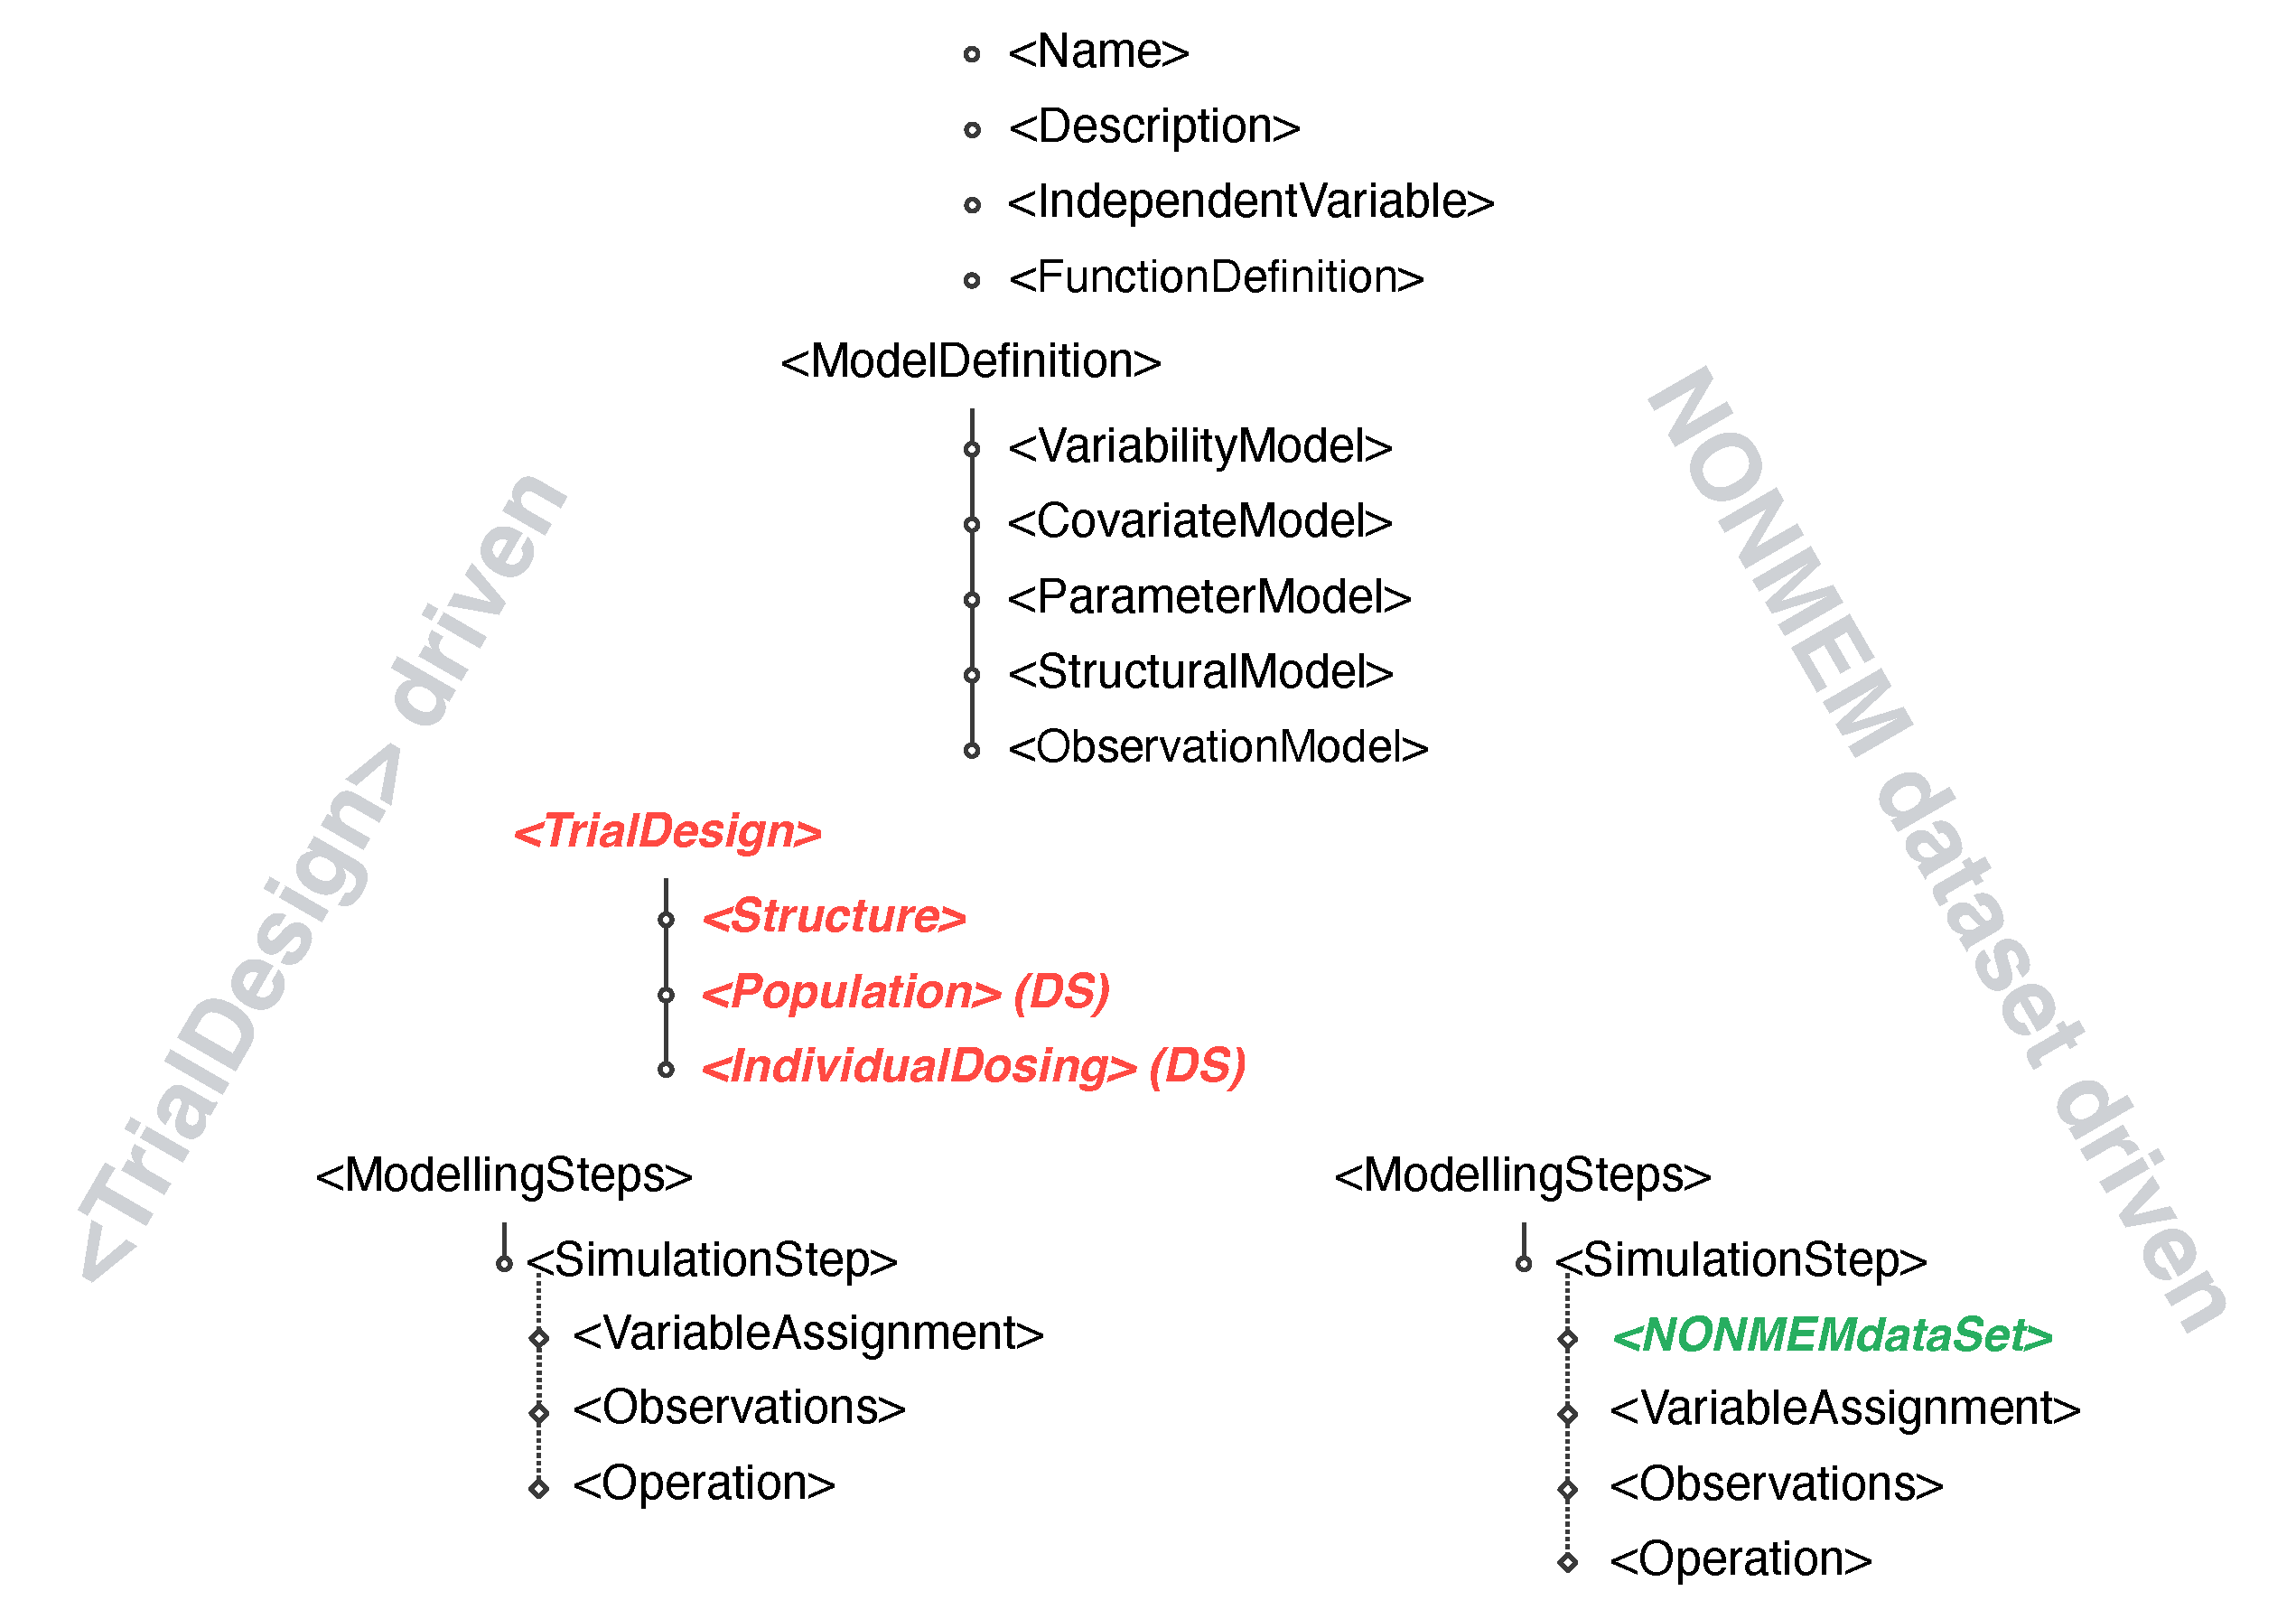
\includegraphics[width=.8\linewidth]{pics/SimulationTask}%
 \caption{PharmML building blocks used for a \textbf{SIMULATION} task implemented 
 using the \xelem{TrialDesign} (left) or NONMEM dataset (right) driven option. 
(DS) indicates that tabular data structure is used.}
 \label{fig:SimulationTask_List}
 \end{figure}
Figures \ref{fig:EstimationTask_List} and \ref{fig:SimulationTask_List} show 
an comparison in the structure to be implemented for typical simulation 
and estimation tasks.
Colours underline elements where the structure of 
\pharmml for these tasks differs dependent whether the \xelem{TrialDesing}
or NONMEM datasets are used to inform the model about the underlying 
study design and experimental data.

\begin{figure}[htb!]
 \centering	
 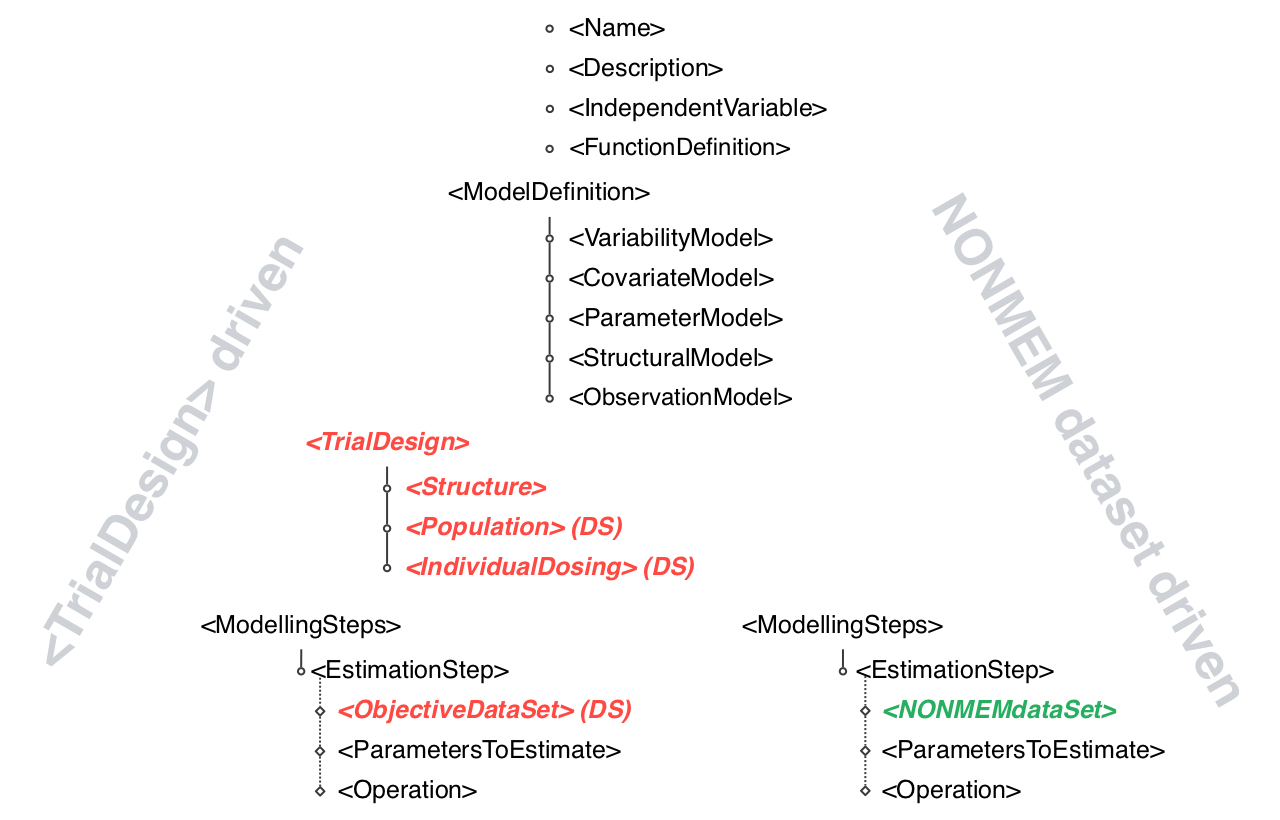
\includegraphics[width=.8\linewidth]{pics/EstimationTask}%
 \caption{PharmML building blocks used for an \textbf{ESTIMATION} task implemented 
 using the \xelem{TrialDesign} (left) or NONMEM dataset (right) driven option. 
(DS) indicates that tabular data structure is used.}
 \label{fig:EstimationTask_List}
 \end{figure}
The following sections will provide two versions of a number of simulation and estimation 
examples, each with the complete description of the according model, trial design 
and task implementation. 

%%%%%%%%%%%%%%%%%%%%%%%%%%%%%%%%%%%%%%%%%%%%%%%%%%%%%%%%%%%%%%%%%%%%%
%%%%%%%%%%%%%%%%%%%%%%%%%%%%%%%%%%%%%%%%%%%%%%%%%%%%%%%%%%%%%%%%%%%%%
\eglabel{1}
\section{Example \theexamples: Simulation, PK + PD response}
\label{sec:eg1}

The following example\footnote{The example is encoded in two versions,  
\xatt{example1.xml} and \xatt{example1\_NONMEM.xml}, with explicit encoded trial 
design and design sourced from a NONMEM datafile, respectively.} is 
based on the CTS1 use case \cite{Lavielle:2011}. Both PK (the drug 
concentration) and PD (the drug effect) are simulated. A one compartment 
PK model is linked to an indirect response PD model, see Figure 
\ref{fig:simplePKPD} for a typical simulation result for one patient.

\begin{figure}[ht!]
\begin{center}
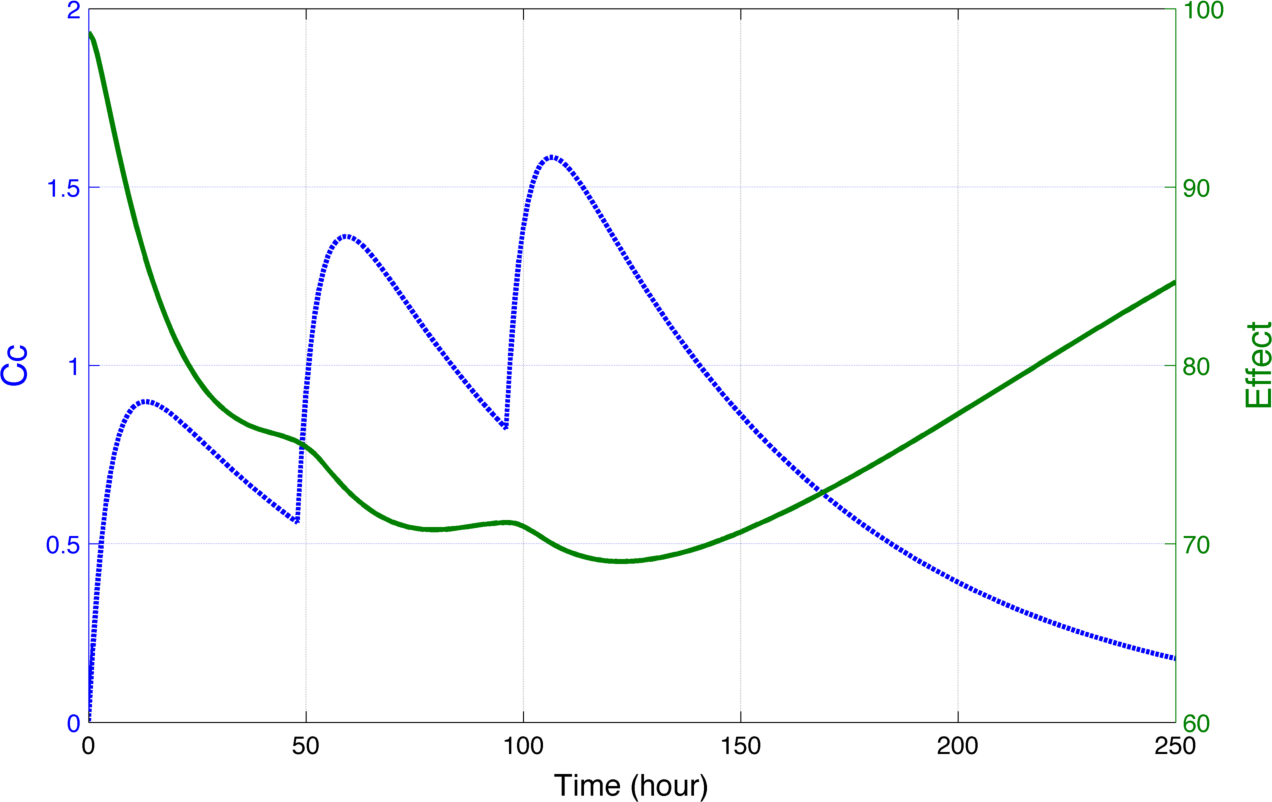
\includegraphics[width=.45\textwidth]{pics/CTS1_smallPKPD}
\caption{Simulated combined model as defined in the example with PK (blue) and PD (green) time courses for one subject. Here three doses were administered every $48h$.}
\label{fig:simplePKPD}
\vspace{-20pt}
\end{center}
\end{figure}

%%%%%%%%%%%%%%%%%%%%%%%%%%%%%%%%%%%%%%%%%%%%%%%%%%%%%%%%%%%%%%%%%%%%%
\subsection{Model Definition}

\subsubsection{Structural model}
This is an oral one compartment model and an indirect response model
with parameters \var{ka}, \var{V}, \var{CL}, \var{Imax}, \var{IC50},
\var{Rin} and \var{kout}.

\begin{align}
k&=\frac{\CL}{V}  \label{eqn:eg1-struct-model}\\
\frac{dAd}{dt} &=-ka \times Ad  \nonumber\\
\frac{dAc}{dt}&=ka \times Ad - k \times Ac  \nonumber\\
\frac{dE}{dt} &=Rin \times \Bigg(1-\frac{\Imax \times \Cc}{\Cc+\IC50}\Bigg)
- kout \times E \nonumber\\
\Cc &= \frac{Ac}{V} \nonumber
\intertext{initial conditions:}
E(t=0) &= \frac{Rin}{kout}  \label{eqn:eg1-init-conds}\\
Ad(t=0) &= 0  \nonumber\\
Ac(t=0) &= 0 \nonumber
\end{align}


\subsubsection{Covariate model}

The only covariate is Weight, $W$, and it is a continuous covariate:
\begin{gather}
W \sim \mathcal{N}(\pop_{\Weight}, \omega_{\Weight}) \label{eqn:eg1-covariate-defn}
\intertext{The following transformation is applied:}
\log(\Weight/70) \label{eqn:eg1-covariate-trans}
\intertext{and the initial values are:}
\pop_{\Weight} =70.07, \quad \omega_{\Weight} =14.09 \nonumber
\end{gather}

\subsubsection{Parameter model}

\paragraph{PK parameters}

The model uses the following individual parameters:
\begin{description}
\item[\var{ka}] absorption rate constant
\item[\var{V}] volume of distribution
\item[\var{CL}] clearance of elimination
\end{description}
All follow a log-normal distribution:
\begin{align}
\log(ka_{i}) &=  \log(\pop_{ka}) + \eta_{ka,i}   \label{eqn:eg1-param-ka}\\
\log(V_i) &= \log(\pop_{V}) + \beta_{1,V}\log(W_i/70) + \eta_{V,i}   \label{eqn:eg1-param-V}\\
\log(\CL_i) &=  \log(\pop_{\CL}) + \beta_{1,\CL}\log(W_i/70) +
\eta_{\CL,i} \nonumber
\end{align}
where
\begin{gather*}
\eta_{ka,i} \sim N(0, \omega_{ka}), \quad \eta_{V,i} \sim N(0,
\omega_{V}), \quad \eta_{\CL,i} \sim N(0, \omega_{\CL})
\intertext{with initial values:}
\pop_{ka}=1,\quad \omega_{ka}=0.6  \qquad \pop_V=8,\quad \omega_V=0.2 \\
\pop_{\CL}=0.13,\quad \omega_{\CL}=0.2  \qquad \beta_{1,V}=1 , \quad \beta_{1,\CL}=0.75  \\
\rho_{V,\CL}=0.7\footnotemark
\end{gather*}
\footnotetext{Correration coefficient between $\eta_{V,i}$ and $\eta_{\CL,i}$}

\paragraph{PD parameters}

The model uses the following individual parameters:
\begin{description}
\item[\var{Imax}] maximal antagonistic response
\item[\var{IC50}] concentration giving half the maximal response
\item[\var{Rin}] input (synthesis) rate
\item[\var{kout}] output (elimination) rate
\end{description}
All follow a log-normal distribution, except \var{Imax}, which follows a logit-normal distribution.
\begin{align*}
\logit(Imax_i) =& \logit(\pop_{Imax})  + \eta_{Imax,i}   \\
\log(\IC50_{i}) =& \log(\pop_{\IC50}) + \eta_{\IC50,i}  \\
\log(\Rin_i) =& \log(\pop_{\Rin}) + \eta_{\Rin,i}  \\
\log(\kout_i) =& \log(\pop_{\kout}) + \eta_{\kout,i}
\end{align*}
where
\begin{gather*}
  \eta_{Imax,i} \sim N(0, \omega_{Imax}), \quad \eta_{\IC50,i} \sim
  N(0, \omega_{\IC50}), \\
\eta_{\Rin,i} \sim N(0, \omega_{\Rin}), \quad \eta_{\kout,i} \sim N(0, \omega_{\kout})
\intertext{with initial values:}
\pop_{Imax} =0.9,\quad \omega_{Imax}=2  \qquad \pop_{\IC50} =
0.4,\quad \omega_{\IC50} =0.4  \\
\pop_{\Rin}=5, \quad \omega_{\Rin}=0.05  \qquad \pop_{\kout} =0.05,
\quad \omega_{\kout} =0.05
\end{gather*}

\paragraph{Variance-covariance matrix}
\label{sec:covariance-matrix}
The full variance-covariance matrix for the random effects is:
\begin{gather}
 \Omega =
 \begin{pmatrix}
  \omega_{ka}^2 	& 0 				& 0  				& 0  				& 0  				& 0  				& 0  				\\
   			  	& \omega_{V}^2	& \omega_{V,\CL} 	& 0  				& 0  				& 0  				& 0  				\\
  				& 				& \omega_{\CL}^2	& 0  				& 0  				& 0  				& 0  				\\
 				&				&   				& \omega_{Imax}^2  & 0  				& 0  				& 0  				\\
				&   				&   				&   				& \omega_{IC50}^2  & 0  				& 0  				\\
				&   				&   				&   				&   				& \omega_{Rin}^2 	& 0  				\\
				&   				&   				&   				&   				&   				& \omega_{kout}^2
 \end{pmatrix}
\intertext{where}
\omega_{V,\CL} = \omega_\var{V} \, \omega_{\CL} \,\rho_{\var{V},\CL}\nonumber
\label{sec:eg-covariance-mat}
\end{gather}

\subsubsection{Observation model}
\label{sec:eg1-desc-obs-model}

We apply a residual error model to the output variables \var{Cc} and \var{E}
from the PK and PD models respectively.

%\begin{table*}[h!]
\begin{center}
\small
\renewcommand{\arraystretch}{1.1}% 
\begin{tabular*}{0.8\linewidth}{@{\extracolsep{\fill}} >{\bfseries}l l l}\toprule
Output Variable & \textbf{\itshape Cc} &\textbf{\itshape E}\\\midrule
Observation Name & Concentration & PCA\\
Units & $\mg/l$ & $\%$\\
Type & Continuous & Continuous \\
Model & Combined & Constant \\
Parameters & $a = 0.5,\quad b=0.1$ & $a=4$\\
\bottomrule
\end{tabular*}
\end{center}

%%%%%%%%%%%%%%%%%%%%%%%%%%%%%%%%%%%%%%%%%%%%%%%%%%%%%%%%%%%%%%%%
\subsection{Trial Design}
\label{subsec:exp2_TaskDescription}

\begin{figure}[h!]
\centering
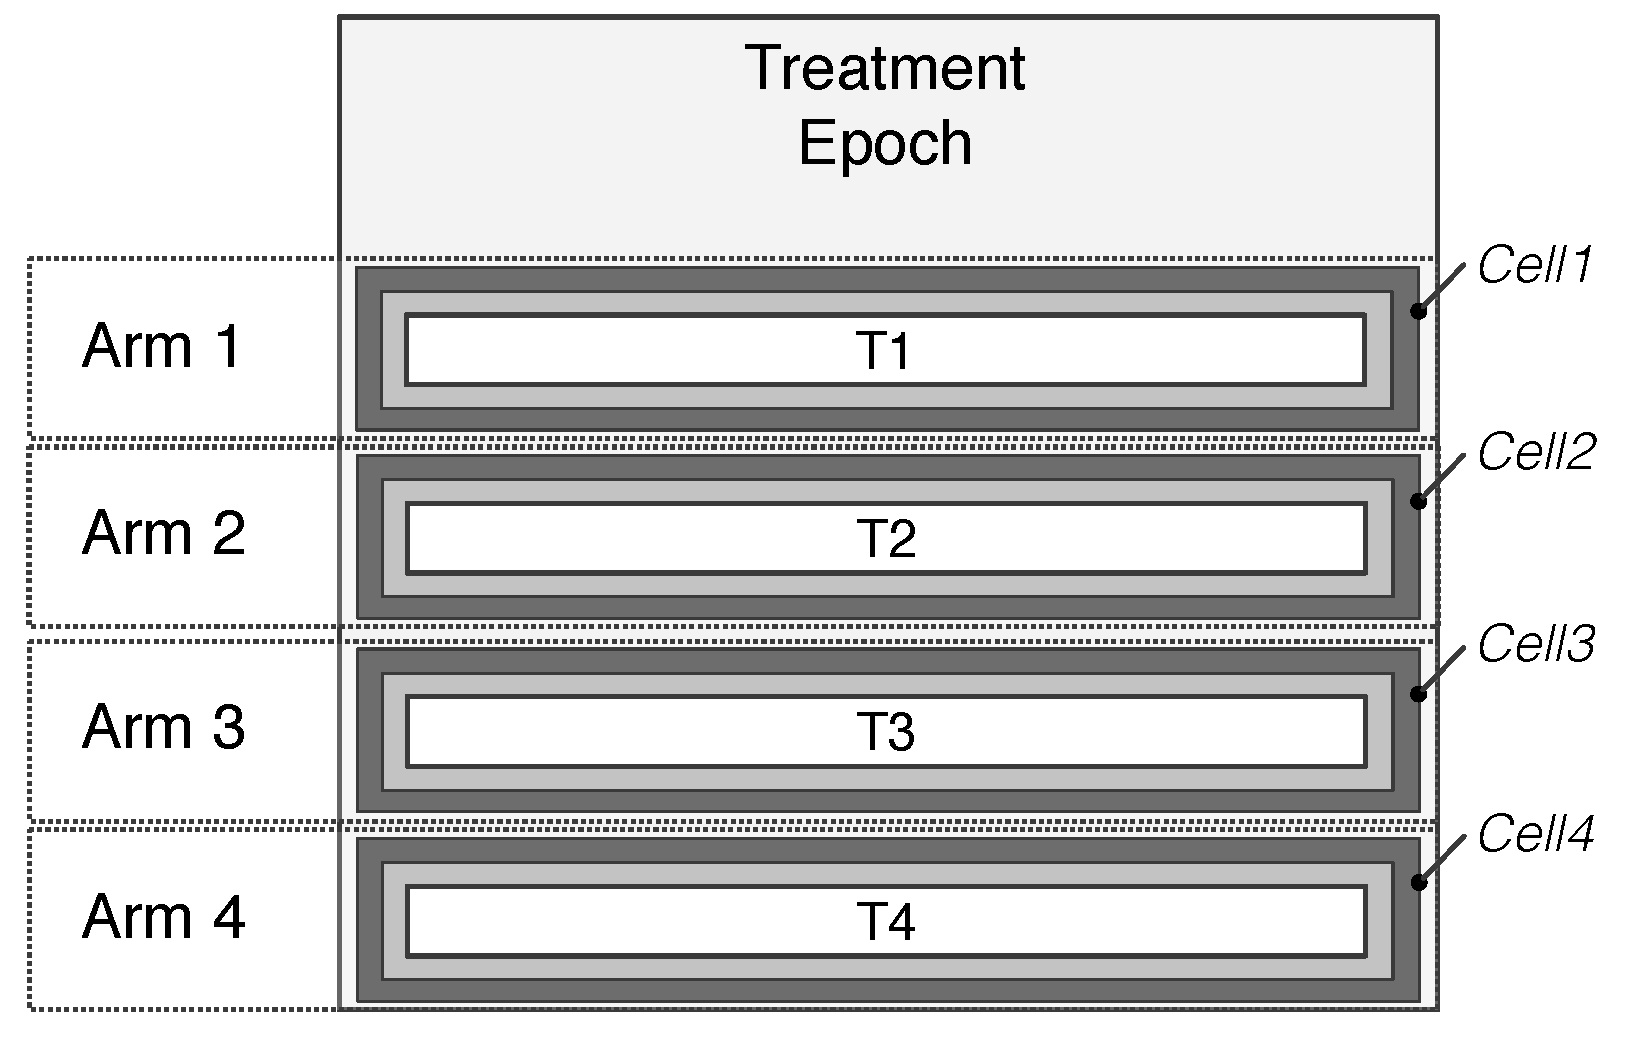
\includegraphics[width=0.7\linewidth]{pics/FourArmsOneEpoch}
\caption{Design overview: this study consists of four arms and one epoch. 
The differences between arms lie in the number of subjects, dose amount and 
times. See table below for the details.}
\label{fig:designPattern_4Arms1Epoch}
\end{figure}

Figure \ref{fig:designPattern_4Arms1Epoch} shows the \textit{Structure} of
this example consisting of four arms and one epoch, meaning there are four treatment
types for which only one time period needs to be specified.

The dosing regimen for the trial is given for each arm below. Note
that all dosing is bolus dosing (discrete administration at specific
times) and all doses are administered to the same compartment.

%\begin{table*}[h!]
\begin{center}
\small
\renewcommand{\arraystretch}{1.1}% 
\begin{tabular*}{0.9\linewidth}{@{\extracolsep{\fill}} >{\bfseries}l rrrr}\toprule
Arm & \textbf{1} &\textbf{2} &\textbf{3} & \textbf{4}\\ \midrule
Number of subjects & 20 & 20 & 40 & 40 \\
Dose target & \var{Ad} & \var{Ad} & \var{Ad} & \var{Ad}\\
Dosing Amount & 0.25 & 0.5 & 0.5 & 1\\
Dose Units & $\mg/\kg$  & $\mg/\kg$  & $\mg/\kg$  & $\mg/\kg$ \\
Dose per kg & yes & yes & yes & yes\\
Dosing times (h) & 0:24:192 &  0:48:192 &  0:24:192 & 0:48:192 \\
\bottomrule
\end{tabular*}
\end{center}


%%%%%%%%%%%%%%%%%%%%%%%%%%%%%%%%%%%%%%%%%%%%%%%%%%%%%%%%%%%%%%%%
\subsection{Modelling Steps}

Time of measurement for PK and PD happens according to different
schedules and these observation time points are produced by the
simulation. The output variables to be generated by the simulation and
their associated time points are shown below:

\begin{center}
\small
\renewcommand{\arraystretch}{1.1}% 
\begin{tabular*}{0.9\linewidth}{@{\extracolsep{\fill}} >{\bfseries}l c c}\toprule
Output Variable & \textbf{\itshape Cc} &\textbf{\itshape E}\\\midrule
Observation times & [0.5,4 : 4 : 48, 52 : 24 : 192, 192 : 4 : 250] & 0 : 24 : 288\\
\bottomrule
\end{tabular*}
\end{center}

%%%%%%%%%%%%%%%%%%%%%%%%%%%%%%%%%%%%%%%%%%%%%%%%%%%%%%%%%%%%%%%%
\subsection{\pharmml Document Structure}
\label{sec:symbol-defn}
An overview of the model with the key sections collapsed  as shown in this listing
%\inputxml{exp1_lst1.xml}
\lstset{language=XML}
\begin{lstlisting}
<PharmML xmlns:xsi="http://www.w3.org/2001/XMLSchema-instance"
    xmlns="http://www.pharmml.org/pharmml/0.6/PharmML"
    xsi:schemaLocation="http://www.pharmml.org/pharmml/0.6/PharmML http://www.pharmml.org/pharmml/0.6/PharmML"
    xmlns:math="http://www.pharmml.org/pharmml/0.6/Maths"
    xmlns:ct="http://www.pharmml.org/pharmml/0.6/CommonTypes"
    xmlns:ds="http://www.pharmml.org/pharmml/0.6/Dataset"
    xmlns:mdef="http://www.pharmml.org/pharmml/0.6/ModelDefinition"
    xmlns:mstep="http://www.pharmml.org/pharmml/0.6/ModellingSteps"
    xmlns:mml="http://www.pharmml.org/pharmml/0.6/PharmML"
    implementedBy="MJS" writtenVersion="0.5.1" 
    metadataFile="example1.rdf" id="i1">
    <ct:Name>Example 1 - simulation continuous PK/PD</ct:Name>
    <IndependentVariable symbId="t"/>
    <FunctionDefinition xmlns="http://www.pharmml.org/pharmml/0.6/CommonTypes" 
    	symbId="constantErrorModel" symbolType="real">
        <!-- omitted details -->
    </FunctionDefinition>
    <FunctionDefinition xmlns="http://www.pharmml.org/pharmml/0.6/CommonTypes" 
    	symbId="combinedErrorModel" symbolType="real">
        <!-- omitted details -->
    </FunctionDefinition>
    <ModelDefinition xmlns="http://www.pharmml.org/pharmml/0.6/ModelDefinition">
        <!-- omitted details -->
    </ModelDefinition>
    <TrialDesign xmlns="http://www.pharmml.org/pharmml/0.6/TrialDesign">
        <!-- omitted details -->
    </TrialDesign>
    <ModellingSteps xmlns="http://www.pharmml.org/pharmml/0.6/ModellingSteps">
        <!-- omitted details -->
    </ModellingSteps>
</PharmML>
\end{lstlisting}


illustrates the main sections of the model as described
in Section \ref{sec:structure-overview}. The key points to note are
the use of the \xelem{IndependentVariable}  element to set the time
variable to $t$ (c.f.\xspace section \ref{sec:independent-var}), and
how the element \xelem{Name} defines the name of the model. In addition
the top-level \xelem{PharmML} element contains a number of attributes
prefixed \texttt{xmlns} (\texttt{xmlns} stands for XML namespace.). These 
are required by the XML Schema standard
and can be ignored as we go through the examples\footnote{To learn more 
about the technical aspects of XML and the XML Schema standard
  used to define \pharmml then the recommend place to start is:
  \url{http://www.w3.org/TR/xmlschema-0/}.}.

Few attributes are use, such as
\begin{itemize}
\item
\xatt{implementedBy} -- to identify the person who implemented the model
\item
\xatt{writtenVersion} -- to identify the \pharmml version
\item
\xatt{metadataFile} -- specifies the optional RDF file associated with the model
introduced in Section \ref{sec:annotation}
\item
\xatt{id} -- metadata element, described in Section \ref{sec:element-id}.
\end{itemize}

The following listing introduces the \xelem{FunctionDefinition} element. 
It defines a function that returns a real type as shown in the following listing 
\lstset{language=XML}
\begin{lstlisting}
    <FunctionDefinition xmlns="http://www.pharmml.org/pharmml/0.6/CommonTypes" 
    	symbId="combinedErrorModel" symbolType="real">
        <FunctionArgument symbId="a" symbolType="real"/>
        <FunctionArgument symbId="b" symbolType="real"/>
        <FunctionArgument symbId="f" symbolType="real"/>
        <Definition>
            <Equation xmlns="http://www.pharmml.org/pharmml/0.6/Maths">
                <Binop op="plus">
                    <ct:SymbRef symbIdRef="a"/>
                    <Binop op="times">
                        <ct:SymbRef symbIdRef="b"/>
                        <ct:SymbRef symbIdRef="f"/>
                    </Binop>
                </Binop>
            </Equation>
        </Definition>
    </FunctionDefinition>
\end{lstlisting}

The function takes three arguments of scalar type and defines the
function:
\begin{displaymath}
\var{combinedError}(a, b, f) = a + bf
\end{displaymath}
This function is used to encode the combined error model function used later in
the observation model (see Section \ref{sec:eg1-obs-model}).


%%%%%%%%%%%%%%%%%%%%%%%%%%%%%%%%%%%%%%%%%%%%%%%%%%%%%%%%%%%%%%%%
\subsection{Model Definition}

As you can see in the following listing 
%\inputxml{exp1_lst3.xml}
\lstset{language=XML}
\begin{lstlisting}
    <ModelDefinition xmlns="http://www.pharmml.org/pharmml/0.6/ModelDefinition">
        <VariabilityModel blkId="vm1" type="parameterVariability">
            <!-- omitted details -->
        </VariabilityModel>
        <VariabilityModel blkId="vm2" type="residualError">
            <!-- omitted details -->
        </VariabilityModel>
        <CovariateModel blkId="cm1">
            <!-- omitted details -->
        </CovariateModel>
        <ParameterModel blkId="p1">
            <!-- omitted details -->
        </ParameterModel>
        <StructuralModel blkId="sm1">
            <!-- omitted details -->
        </StructuralModel>
        <ObservationModel blkId="om1">
            <!-- omitted details -->
        </ObservationModel>
        <ObservationModel blkId="om2">
            <!-- omitted details -->
        </ObservationModel>
    </ModelDefinition>
\end{lstlisting}
the model definition section defines the main components that you will see in
the subsequent examples. All of these elements are optional and all follow the 
scoping rules described in section \ref{sec:blocks}.


%%%%%%%%%%%%%%%%%%%%%%%%%%%%%%%%%%%%%%%%%%%%%%%%%%%%%%%%%%%%%%%%
\subsubsection{Variability Model}
\label{sec:eg1-variability}
\begin{figure}[ht!]
\centering
 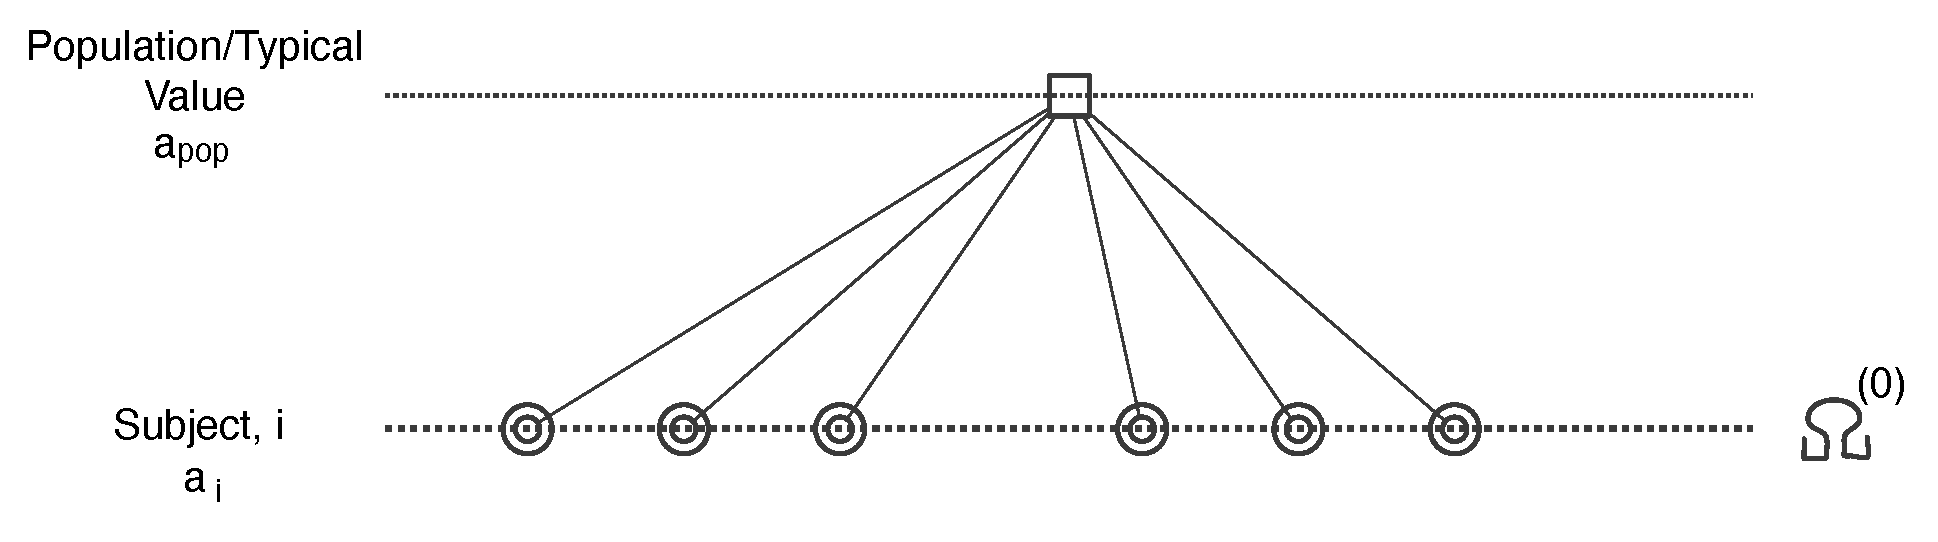
\includegraphics[width=130mm]{pics/IOV0}
\caption{There is only one level of variability in this example -- inter-individual variability.}
\label{fig:tree_IOV0}
\end{figure}
From the following listing one can also see that there
are two variability models defined using the element
\xelem{Vari\-abilityModel}. This is how we explicitly define the
level of variability in the model (c.f.\ section
\ref{sec:variabilityModel}). In this case there is one level of 
variability, the inter-individual, Figure \ref{fig:tree_IOV0} and the residual
error model variability, see the following listing 
%\inputxml{exp1_lst3A.xml}
\lstset{language=XML}
\begin{lstlisting}
    <VariabilityModel blkId="vm1" type="parameterVariability">
        <Level referenceLevel="true" symbId="indiv">
            <ct:Name>Individual Variability</ct:Name>
        </Level>
    </VariabilityModel>
    <VariabilityModel blkId="vm2" type="residualError">
        <Level symbId="residual">
            <ct:Name>Residual Error</ct:Name>
        </Level>
    </VariabilityModel>
\end{lstlisting}
for the details of the implementation. Please, note that we use two different variability 
attribute types, \xatt{parameterVariability} and \xatt{residualError}. The former stands for random variability
associated with the parameters, as described in section \ref{sec:variabilityModel}. 
For this example we are defining one level of variability in the parameter model and this
corresponds to variability between subjects. The latter stands for residual error variability.

The attribute \xatt{referenceLevel="true"} identifies the \xatt{indiv} level as the reference level.
This attribute is not required if there is only one level and the proper mapping from the 
dataset or \xelem{Population} in the \xelem{TrialDesign} section is defined. However it is 
required if a model is implemented using the \xelem{ModelDefinition} section only.
This will be explained again when dealing with examples with more complex variability models (section \ref{eg4:variabilityModel}).

%%%%%%%%%%%%%%%%%%%%%%%%%%%%%%%%%%%%%%%%%%%%%%%%%%%%%%%%%%%%%%%%
\subsubsection{Covariate Model}
\label{sec:eg1-covariate}


The \xelem{CovariateModel} block corresponds to the covariate model
defined in section \ref{maths:covariate_model}. In this example, as shown
in this listing 
%\inputxml{exp1_lst4and5.xml}
\lstset{language=XML}
\begin{lstlisting}
        <CovariateModel blkId="cm1">
            <SimpleParameter symbId="pop_W"/>
            <SimpleParameter symbId="omega_W"/>
            <Covariate symbId="W">
                <Continuous>
                    <NormalDistribution xmlns="http://www.uncertml.org/3.0" 
                    		definition="http://www.uncertml.org/distributions/normal">
                        <mean>
                            <var varId="pop_W"/>
                        </mean>
                        <variance>
                            <var varId="omega_W"/>
                        </variance>
                    </NormalDistribution>
                    <Transformation>
                        <TransformedCovariate symbId="logW70"/>
                        <Equation xmlns="http://www.pharmml.org/pharmml/0.6/Maths">
                            <Uniop op="log">
                                <Binop op="divide">
                                    <ct:SymbRef symbIdRef="W"/>
                                    <ct:Real>70.0</ct:Real>
                                </Binop>
                            </Uniop>
                        </Equation>
                    </Transformation>
                </Continuous>
            </Covariate>
        </CovariateModel>
\end{lstlisting}
we are defining a continuous covariate, \var{W}, indicated by the 
\xelem{Continuous} element and the covariate is sampled from a 
normal distribution as in equation \ref{eqn:eg1-covariate-defn}.  
The element \xelem{Transformation} beneath the definition of the 
distribution describes the transformation applied to this covariate. 
We can either refer to the untransformed or transformed form of the 
covariate whatever form is required. The later will be refered to as 
\emph{logW70} as defined in the \xelem{TransformedCovariate} element. 
In this case the transformation being 
applied is defined in equation~\ref{eqn:eg1-covariate-trans}.


%%%%%%%%%%%%%%%%%%%%%%%%%%%%%%%%%%%%%%%%%%%%%%%%%%%%%%%%%%%%%%%%
\subsubsection{Parameter Model}
\label{sec:eg1-pk}
All parameters in the current example can be defined
using the Gaussian model with linear covariates (see section
\ref{sec:parameterModel}). We will start with a simple case in this
example, shown in the following listing 
%\inputxml{exp1_lst6.xml}
\lstset{language=XML}
\begin{lstlisting}
    <ParameterModel blkId="p1">
        <!-- omitted other parameters -->
        <!-- ka -->
        <SimpleParameter symbId="pop_ka"/>
        <SimpleParameter symbId="omega_ka"/>
        <RandomVariable symbId="eta_ka">
            <ct:VariabilityReference>
                <ct:SymbRef blkIdRef="vm1" symbIdRef="indiv"/>
            </ct:VariabilityReference>
            <NormalDistribution xmlns="http://www.uncertml.org/3.0" 
                definition="http://www.uncertml.org/distributions/normal">
                <mean><rVal>0</rVal></mean>
                <stddev><var varId="omega_ka"/></stddev>
            </NormalDistribution>
        </RandomVariable>
        <IndividualParameter symbId="ka">
            <GaussianModel>
                <Transformation>log</Transformation>
                <LinearCovariate>
                    <PopulationParameter>
                        <ct:Assign>
                            <ct:SymbRef symbIdRef="pop_ka"/>
                        </ct:Assign>
                    </PopulationParameter>
                </LinearCovariate>
                <RandomEffects>
                    <ct:SymbRef symbIdRef="eta_ka"/>
                </RandomEffects>
            </GaussianModel>
        </IndividualParameter>
\end{lstlisting}
the absorption rate constant \var{ka}.  First the typical value for \var{ka}, \var{pop\_ka}
and the standard deviation of the random effect, \var{omega\_ka}, are
defined as \xelem{SimpleParameter}'s. Then the random effect \var{eta\_ka}
is defined, which follows a normal distribution with mean $0$ and
standard deviation \var{omega\_ka}.

Then the actual individual parameter \var{ka} is
defined with the \xelem{Transformation} attribute set to
\texttt{log}. This tells us that the parameter is log-transformed. We
are using the Gaussian model described previously (section
\ref{maths:parameter-model}), and it follows a log-normal distribution
with the mean \var{pop\_ka} and the standard deviation
 \var{omega\_ka}, as shown in equation \ref{eqn:eg1-param-ka}.
Even though \var{ka} is modelled without a covariate, we still use the
element \xelem{LinearCovariate}, which contains here logically only the
typical value element \xelem{PopulationParameter}.

The \xelem{RandomVariable} element is very important here. It tells us
what the random effect is, and, by assigning a variability level to
the attribute \xatt{symbIdRef} within the \xelem{VariabilityRef\-erence} element,
it effectively tells us that the random effect is sampled for every subject.
The importance of this will become clearer in later examples that describe
multiple levels of variability. Note that the \xelem{RandomVariable} element
also defines a new symbol \var{eta\_ka}, which is a parameter.


Of course not all parameter definitions are so straight forward. In the
following listing 
%\inputxml{exp1_lst7.xml}
\lstset{language=XML}
\begin{lstlisting}
    <ParameterModel blkId="p1">
        <!-- V -->
        <SimpleParameter symbId="beta_V"/>
        <SimpleParameter symbId="pop_V"/>
        <SimpleParameter symbId="omega_V"/>
        <RandomVariable symbId="eta_V">
            <ct:VariabilityReference>
                <ct:SymbRef blkIdRef="vm1" symbIdRef="indiv"/>
            </ct:VariabilityReference>
            <NormalDistribution xmlns="http://www.uncertml.org/3.0" 
                definition="http://www.uncertml.org/distributions/normal">
                <mean><rVal>0</rVal></mean>
                <stddev><var varId="omega_V"/></stddev>
            </NormalDistribution>                            
        </RandomVariable>
        <IndividualParameter symbId="V">
            <GaussianModel>
                <Transformation>log</Transformation>
                <LinearCovariate>
                    <PopulationParameter>
                        <ct:Assign>
                            <ct:SymbRef symbIdRef="pop_V"/>
                        </ct:Assign>
                    </PopulationParameter>
                    <Covariate>
                        <ct:SymbRef blkIdRef="cm1" symbIdRef="logW70"/>
                        <FixedEffect>
                            <ct:SymbRef symbIdRef="beta_V"/>
                        </FixedEffect>
                    </Covariate>
                </LinearCovariate>
                <RandomEffects>
                    <ct:SymbRef symbIdRef="eta_V"/>
                </RandomEffects>
            </GaussianModel>
        </IndividualParameter>
\end{lstlisting}
you can see the definition of a
parameter, \var{V}, that is related to the covariate, $W$. We do this
using the element \xelem{Covariate} to indicate there is a
relationship. Then we reference the specific covariate (using the
\xelem{SymbRef} element) and describe the fixed effect relating the
covariate to this parameter: in this case we are referring to the
parameter \var{beta\_V}. We define here a linear covariate model
when relating covariates to parameters (c.f.\xspace section
\ref{maths:covariate_model}), so this example corresponds to
equation (\ref{eqn:eg1-param-V}).

Equation (\ref{eqn:eg1-param-V}) uses the transformed covariate 
$\log\left(W/70\right)$ as defined in (\ref{eqn:eg1-covariate-trans}), 
and implemented in the \xelem{CovariateModel} (section \ref{sec:eg1-covariate}).
It is the decision of the modeller whether to use an untransformed or 
transformed form of a covariate and part of the covariate model building. 

Having defined the individual and other parameters in the parameter
model we need to describe the correlation of the random effects, if any.
As described above (see section \ref{subsec:correlationModel} for
a complete description) this is done using a covariance matrix.
In \pharmml, if the random effects of both
parameters follow a normal distribution, then we assume that the
diagonal of the covariance matrix can be derived from the variance or
standard deviation of each parameter (c.f section
\ref{maths:covariance-mat-derivation}). This is true in this example,
so one only needs to define the parts of the covariance structure that
define the correlation between parameters \var{V} and \var{CL}
as shown in this listing 
%\inputxml{exp1_lst8.xml}
\lstset{language=XML}
\begin{lstlisting}
    <Correlation>
        <ct:VariabilityReference>
            <ct:SymbRef blkIdRef="vm1" symbIdRef="indiv"/>
        </ct:VariabilityReference>
        <Pairwise>
            <RandomVariable1>
                <ct:SymbRef symbIdRef="eta_V"/>
            </RandomVariable1>
            <RandomVariable2>
                <ct:SymbRef symbIdRef="eta_Cl"/>
            </RandomVariable2>
            <CorrelationCoefficient>
                <ct:SymbRef symbIdRef="rho_V_Cl"/>
            </CorrelationCoefficient>
        </Pairwise>
    </Correlation>
\end{lstlisting}

With the \xelem{VariabilityReference} element and its \xatt{symbIdRef} 
attribute the correlation is associated with a certain variability level 
as defined at the beginning of the model definition. 
To specify the correlation structure we can either defined the full covariance
matrix using \xelem{Matrix} or as in this case the \xelem{Pairwise} element
because only two random effects are correlated. Accordingly we need to 
define the random effects of interest and either correlation coefficient or
their covariance.
This single \xelem{Correlation} element is all we need to define the sparse 
covariance matrix mentioned above (section \ref{sec:eg-covariance-mat}). 


%%%%%%%%%%%%%%%%%%%%%%%%%%%%%%%%%%%%%%%%%%%%%%%%%%%%%%%%%%%%%%%%
\subsubsection{Structural Model}

In \pharmml the structural model can be described using algebraic
equations or using ODEs/DDEs. In this case the model is defined 
as a combination of algebraic and ODE equations (c.f.\xspace equation \ref{eqn:eg1-struct-model}).
We demonstrate how to encode two different assignment types, e.g.
\begin{align}
k & = Cl / V \nonumber \\
\frac{d \var{Ad}}{dt} 	& = -\var{ka} \times \var{Ad}, \quad Ad(t=0)=0 \nonumber \\
\frac{d \var{Ac}}{dt}	& = ka \times Ad - k \times Ac, \quad Ac(t=0)=0  \nonumber
\end{align}
The following listing 
\lstset{language=XML}
\begin{lstlisting}
        <StructuralModel blkId="sm1">
            <SimpleParameter symbId="k">
                <ct:Assign>
                    <Equation xmlns="http://www.pharmml.org/pharmml/0.6/Maths">
                        <Binop op="divide">
                            <ct:SymbRef blkIdRef="p1" symbIdRef="Cl"/>
                            <ct:SymbRef blkIdRef="p1" symbIdRef="V"/>
                        </Binop>
                    </Equation>
                </ct:Assign>
            </SimpleParameter>
            <ct:DerivativeVariable symbId="Ad" symbolType="real">
                <ct:Assign>
                    <Equation xmlns="http://www.pharmml.org/pharmml/0.6/Maths">
                        <Binop op="times">
                            <Uniop op="minus">
                                <ct:SymbRef blkIdRef="p1" symbIdRef="ka"/>
                            </Uniop>
                            <ct:SymbRef symbIdRef="Ad"/>
                        </Binop>
                    </Equation>
                </ct:Assign>
                <ct:IndependentVariable>
                    <ct:SymbRef symbIdRef="t"/>
                </ct:IndependentVariable>
                <ct:InitialCondition>
                    <ct:InitialValue>
                        <ct:Assign>
                            <ct:Real>0</ct:Real>
                        </ct:Assign>
                    </ct:InitialValue>
                </ct:InitialCondition>
            </ct:DerivativeVariable>
            <!-- omitted dAc/dt = ... --> 
\end{lstlisting}
illustrates how the parameter \var{k} is defined, i.e. as the ratio of $CL$ and $V$, 
which are parameters as well but defined in the \xelem{ParameterModel}, \var{p1}. 
Then the derivative \var{Ad} is defined using the element \xelem{DerivativeVariable}
(see section \ref{sec:odes} for a more detailed explanation)
with $t$ as the independent variable, the time. The absorption parameter \var{ka} 
is again defined in \var{p1}.
Finally the \xelem{InitialValue} element within the \xelem{InitialCondition} defines
the initial value for \var{Ad} at time 0, which is the default 
initial time in \pharmml and doesn't have to be specified in this case explicitly. 
Alternatively, any initial time values can be encoded using \xelem{InitialTime} element.


\subsubsection{Structural model -- using PK macros}
The structural model is this time formulated using the PK macros. 
The PK model corresponds to the ADVAN2/TRANS combination 
in the PREDPP library, see Table \ref{tab:ADVAN_translation}.
Following table shows the two allowed parameterizations for ADVAN2 
and the re-parameterization formula. 
\begin{table}[ht]
\centering
\renewcommand{\arraystretch}{1.1}% 
\begin{tabular*}{.8\textwidth}{@{\extracolsep{\fill} } lll}
  \hline
  \hline
  TRANS1								& TRANS2						& Formula \\
  \hline
K Rate constant of elimination				& CL Clearance 					& K=CL/V \\
									& V Volume of distribution				& \\
\end{tabular*}
\caption{ADVAN2 with two available parameterization routines, TRANS1 and TRANS2.}
\end{table}
\begin{figure}[htbp]
\centering
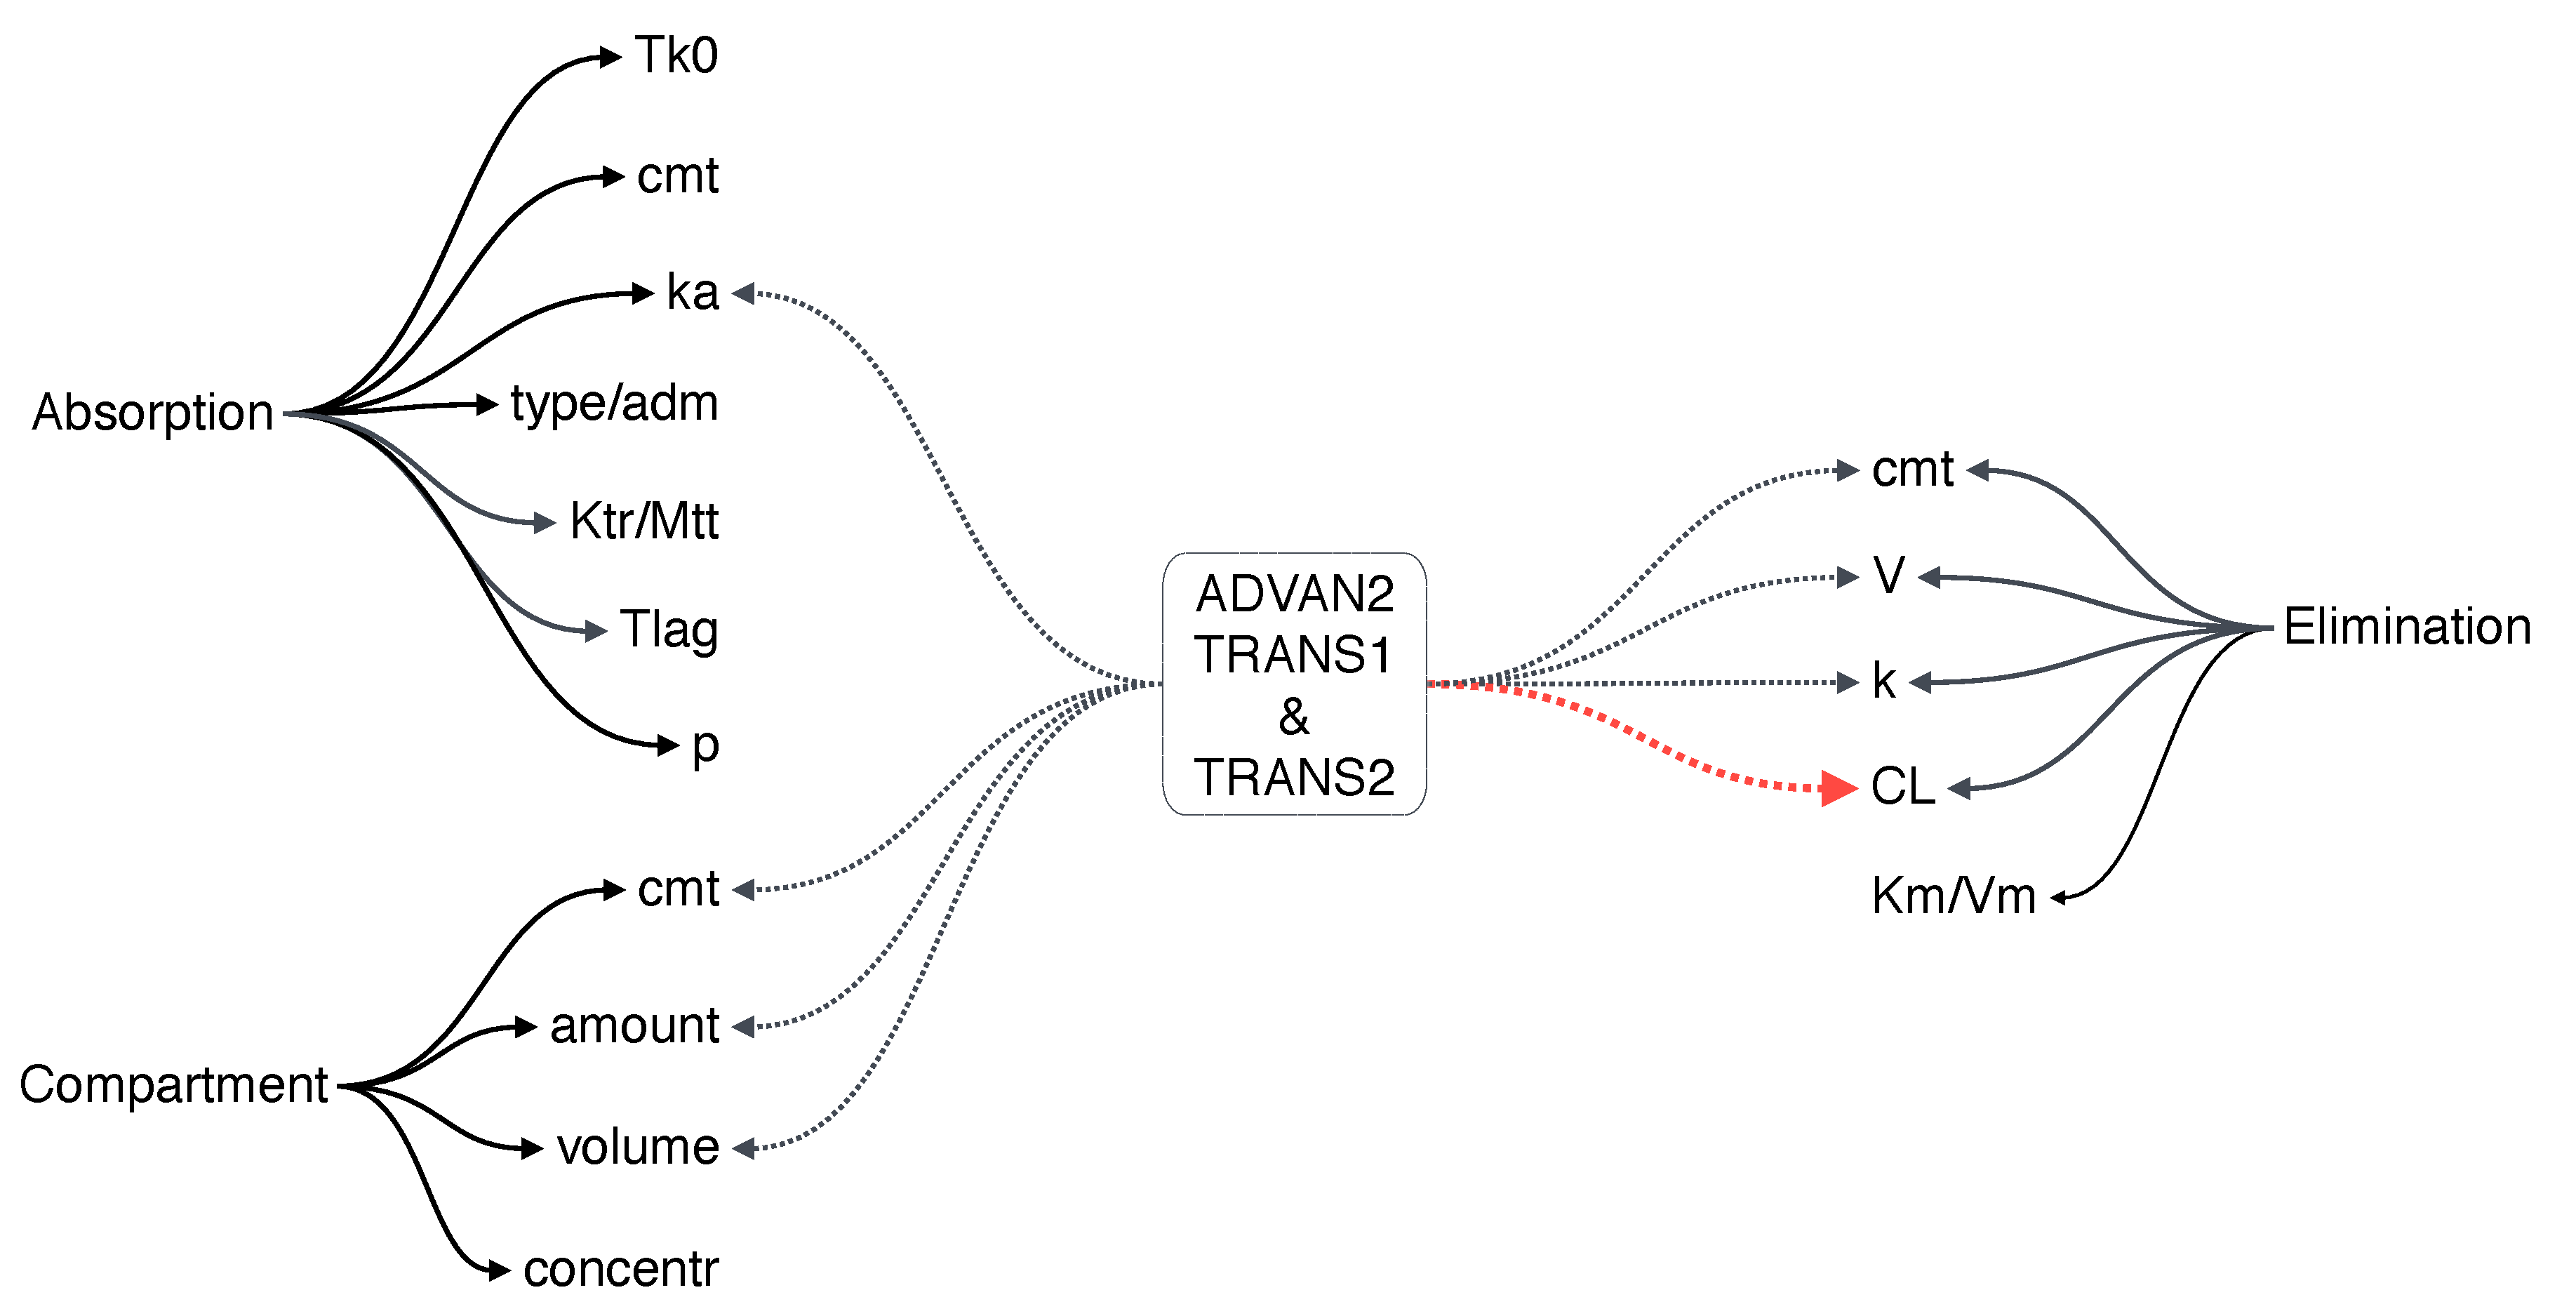
\includegraphics[width=.8\textwidth]{pics/Advan2_Parameterizations}
\caption{Relationship between PK macros and the predefined PREDPP models and 
alternative parameterizations for the structural model, corresponding 
to ADVAN2/TRANS1 and ADVAN2/TRANS2.}
\end{figure}

Table \ref{tab:ADVAN2TRANS1reparameterisation} shows the PK macros for the two options
\begin{table}[ht]
\centering
\renewcommand{\arraystretch}{1.1}% 
\begin{tabular*}{.9\textwidth}{@{\extracolsep{\fill} } ll}
  \hline
  \hline
ADVAN2, TRANS1 & ADVAN2, TRANS2 \\
  \hline
\lstset{language=NONMEMdataSet}
\begin{lstlisting}
compartment(cmt=1, amount=Ac, volume=V)
oral(cmt=1,ka)
elimination(cmt=1, k)
Cc = Ac/V
\end{lstlisting}
&
\lstset{language=NONMEMdataSet}
\begin{lstlisting}
compartment(cmt=1, amount=Ac, volume=V)
oral(cmt=1,ka)
elimination(cmt=1, CL)
Cc = Ac/V
\end{lstlisting}
\end{tabular*}
\caption{The set of macros for the PK model with additional equation for the 
concentration, $Cc$. It corresponds to a ADVAN2/TRANS2 model, see 
Section \ref{subsec:PREDPPinMACROS} and Table \ref{tab:ADVAN_translation} 
for detailed description. Here the two allowed parameterizations are used.}
\label{tab:ADVAN2TRANS1reparameterisation}
\end{table}
and the following code snippet shows how this can be encoded in \pml
\lstset{language=XML}
\begin{lstlisting}
        <StructuralModel blkId="sm1">
            <ct:Variable symbolType="real" symbId="Ac"/>
            <ct:Variable symbolType="real" symbId="Cc">
                <ct:Assign>
                    <math:Equation>
                        <math:Binop op="divide">
                            <ct:SymbRef symbIdRef="Ac"/>
                            <ct:SymbRef blkIdRef="pm1" symbIdRef="V"/>
                        </math:Binop>
                    </math:Equation>
                </ct:Assign>
            </ct:Variable>
            
            <PKmacros>
                <Compartment>
                    <Value argument="cmt">
                        <ct:Int>1</ct:Int>
                    </Value>
                    <Value argument="amount">
                        <ct:SymbRef symbIdRef="Ac"/>
                    </Value>
                    <Value argument="volume">
                        <ct:SymbRef blkIdRef="pm1" symbIdRef="V"/>
                    </Value>
                </Compartment>
                <IV>
                    <Value argument="adm">
                        <ct:Int>1</ct:Int>
                    </Value>
                    <Value argument="cmt">
                        <ct:Int>1</ct:Int>
                    </Value>
                </IV>
                <Elimination>
                    <Value argument="cmt">
                        <ct:Int>1</ct:Int>
                    </Value>
                    <Value>
                        <ct:SymbRef blkIdRef="pm1" symbIdRef="k"/>
                    </Value>
                </Elimination>
            </PKmacros>
        </StructuralModel>
\end{lstlisting}
with the re-paramerization encoded in the \xelem{ParameterModel}, \xatt{pm1}, 
as the following code shows
\lstset{language=XML}
\begin{lstlisting}
        <ParameterModel blkId="pm1">
            <SimpleParameter symbId="V"/>
            <SimpleParameter symbId="CL"/>
            <SimpleParameter symbId="k">
                <ct:Assign>
                    <math:Equation>
                        <math:Binop op="divide">
                            <ct:SymbRef symbIdRef="CL"/>
                            <ct:SymbRef symbIdRef="V"/>
                        </math:Binop>
                    </math:Equation>
                </ct:Assign>
            </SimpleParameter>
            <!-- omitted other parameters and IIV -->

\end{lstlisting}

%%%%%%%%%%%%%%%%%%%%%%%%%%%%%%%%%%%%%%%%%%%%%%%%%%%%%%%%%%%%%%%%
\subsubsection{Observation Model}
\label{sec:eg1-obs-model}

In this example there are two observations for the continuous
variables \var{Cc} and \var{E}, which are outputs from the structural
model. As described above each has a residual error model applied to it.


The XML is very similar for both variables so in the following listing 
\lstset{language=XML}
\begin{lstlisting}
        <ObservationModel blkId="om1">
            <ContinuousData>
                <SimpleParameter symbId="a"/>
                <SimpleParameter symbId="b"/>
                <RandomVariable symbId="epsilon_Cc">
                    <ct:VariabilityReference>
                        <ct:SymbRef blkIdRef="vm2" symbIdRef="residual"/>
                    </ct:VariabilityReference>
                    <NormalDistribution xmlns="http://www.uncertml.org/3.0" 
                    	definition="http://www.uncertml.org/distributions/normal">
                        <mean><rVal>0</rVal></mean>
                        <variance><prVal>1</prVal></variance>
                    </NormalDistribution>
                </RandomVariable>
                <Standard symbId="Cc_obs">
                    <Output>
                        <ct:SymbRef blkIdRef="sm1" symbIdRef="Cc"/>
                    </Output>
                    <ErrorModel>
                        <ct:Assign>
                            <math:Equation>
                                <math:FunctionCall>
                                    <ct:SymbRef symbIdRef="combinedErrorModel"/>
                                    <math:FunctionArgument symbId="a">
                                        <ct:SymbRef symbIdRef="a"/>
                                    </math:FunctionArgument>
                                    <math:FunctionArgument symbId="b">
                                        <ct:SymbRef symbIdRef="b"/>
                                    </math:FunctionArgument>
                                    <math:FunctionArgument symbId="f">
                                        <math:Equation>
                                            <ct:SymbRef blkIdRef="sm1" symbIdRef="Cc"/>
                                        </math:Equation>
                                    </math:FunctionArgument>
                                </math:FunctionCall>
                            </math:Equation>
                        </ct:Assign>
                    </ErrorModel>
                    <ResidualError>
                        <ct:SymbRef symbIdRef="epsilon_Cc"/>
                    </ResidualError>
                </Standard>
            </ContinuousData>
        </ObservationModel>
\end{lstlisting}

we only show how the residual error model for \var{Cc}, the continuous PK variable, is defined.
First the parameters of the residual error model \var{a} and \var{b} are
defined using \xelem{SimpleParameter}; here a combined additive
and proportional error model is applied. Then \var{epsilon\_Cc} as \xelem{RandomVariable}
of the residual error model with a mean of $0$ and standard deviation \var{sigma\_Cc} is defined
to be used in the subsequent parts of the model. Note that we need to 
indicate the type and level of the according random effect which were
defined in the 'Variability Model' section above. This is done
using the \xelem{VariabilityReference} 

The subsequent element \xelem{Standard} states that we are defining a standard
continuous observation model. This means in short that we can define
an observation model of the form $y_{ij} = f_{ij} + g\times\epsilon_{ij}$
(for details, see the discussion below and section \ref{sec:observationModel}).

The attribute \xatt{symbId} of \xelem{Standard} defines the name of the
variable that will hold the result of the applied residual error model.
The \xelem{Output} element then defines the
variable in the structural model that the residual error model applies to
(in this case \var{Cc}). Next we define the actual residual error
model with the \xelem{ErrorModel} element. The error model is invoked
by calling the function \var{combinedErrorModel} defined in the symbol
definition at the beginning of the \pharmml document (see section
\ref{sec:symbol-defn}). We pass in the appropriate parameter values
(see section \ref{maths:combined-err-model} for a description of the
residual error model) and this defines our residual error model.\\
Finally we use the \xelem{ResidualError} element to reference the
\var{epsilon\_Cc} specified before.



%%%%%%%%%%%%%%%%%%%%%%%%%%%%%%%%%%%%%%%%%%%%%%%%%%%%%%%%%%%%%%%%%%
\paragraph{Residual model implementation}
Most residual error model types have two or three equivalent forms, by which 
we mean they have the same variance, although they use one or more residual 
errors, $\epsilon_{ij}$, see examples in section \ref{subsec:modelExamples}. 
Other types contain two or more predictions from the structural model, \var{f_{ij}}. 
From a computational point of view it makes a lot of sense to reflect such 
differences in the language structure.
This was the motivation to allow for the implementation of two types of observation models
\begin{itemize}
\item
\xelem{Standard} -- any observation model of the form
\begin{align*}
	u(y_{ij}) = u(f_{ij}) + g\times\epsilon_{ij}
\end{align*}
which can be defined using exactly one of the following items
\begin{itemize}
\item
a transformation, $u$, e.g. \var{log} or \var{logit}
\item
one structural model prediction, \var{f_{ij}}
\item
one standard deviation function, \var{g}
\item
one random variable, $\epsilon_{ij}$
\end{itemize}
\item
\xelem{General} -- using any number of the items listed above and arbitrary functional relationship between them.
\end{itemize}
This chapter contains more examples illustrating these constructs.

%%%%%%%%%%%%%%%%%%%%%%%%%%%%%%%%%%%%%%%%%%%%%%%%%%%%%%%%%%%%%%%%
\subsection{Trial Design}
\subsubsection{Structure}

In this fairly simple case, there is only one epoch and four arms, \var{Arm\_1}, \var{Arm\_2} etc.,
cf. Figure \ref{fig:designPattern_4Arms1Epoch}.
The resulting four cells \var{Cell\_1}, \var{Cell\_2} etc. each correspond
to one arm and contain one segment.
Figure \ref{fig:CellSegmentEpochArm_example1} (right) illustrates the inter-relationship between
cells, arms, epochs and segments. Here a segment consists of one activity --
a certain type of treatment. In general, a segment can contain more
than one activity. Dosing regimen can be defined for different
compartments in the structural model. In this example there are four
treatments with one dosing regimen per treatment.

\begin{figure}[htbp!]
\centering
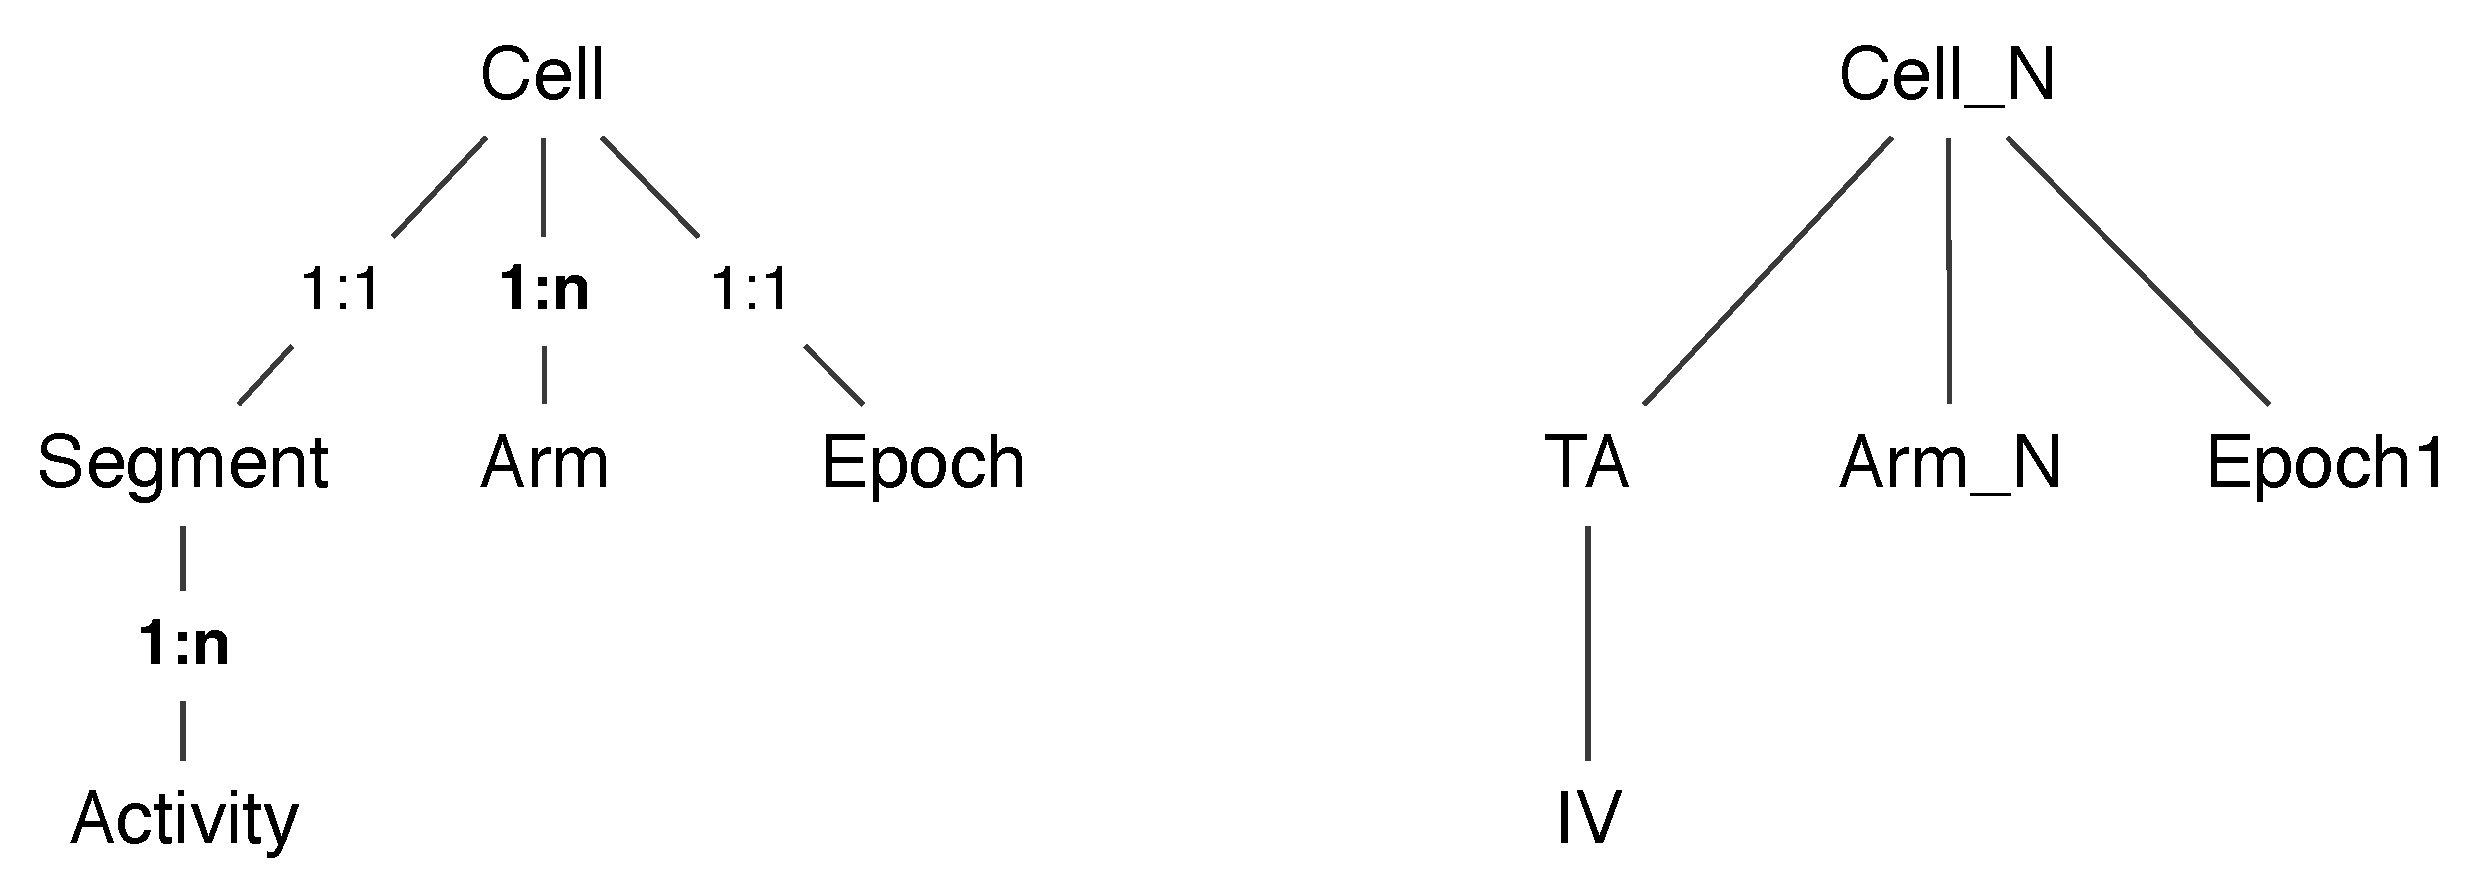
\includegraphics[width=0.7\linewidth]{pics/CellSegmentEpochArm_example1.pdf}
\caption{(left) General cell hierarchy; (right) How it is applied in example (\egref{1}).
There is only one epoch and four arms, \var{Arm\_1}, \var{Arm\_2} etc.
The resulting four cells \var{Cell\_1}, \var{Cell\_2}, etc. each correspond
to one arm and contain one segment. See the listing bellow for how
these features are implemented and structured.}
\label{fig:CellSegmentEpochArm_example1}
\end{figure}

In the following listing 
\lstset{language=XML}
\begin{lstlisting}
            <Activity oid="d1">
                <Bolus>
                    <DoseAmount inputTarget="derivativeVariable">
                        <ct:SymbRef blkIdRef="sm1" symbIdRef="Ad"/>
                        <ct:Assign>
                            <Equation xmlns="http://www.pharmml.org/pharmml/0.6/Maths">
                                <Binop op="times">
                                    <ct:Real>0.25</ct:Real>
                                    <ct:SymbRef blkIdRef="cm1" symbIdRef="W"/>
                                </Binop>
                            </Equation>
                        </ct:Assign>
                    </DoseAmount>
                    <DosingTimes>
                        <ct:Assign>
                            <ct:Sequence>
                                <ct:Begin><ct:Int>0</ct:Int></ct:Begin>
                                <ct:StepSize><ct:Int>24</ct:Int></ct:StepSize>
                                <ct:End><ct:Int>192</ct:Int></ct:End>
                            </ct:Sequence>
                        </ct:Assign>
                    </DosingTimes>
                </Bolus>
            </Activity>
\end{lstlisting}
we show an activity defined for \var{Arm\_1},
here treatment in the form of a bolus administration: the others are very similar.
The \xelem{Activity} element is given an identifier, ``\texttt{d1}'',
and the element \xelem{Bolus} defines a
bolus administration\footnote{Bolus and infusion are the only types of
dosing regimen permitted. We make no distinction between oral and IV
administration as such differences are handled by the structural
model used.}.  \xelem{DoseAmount} defines the amount of drug to be
administered. The are four options here. The dose can be assigned
to the variable defined by an ODE, such is the case here, for which we use
\xatt{inputTarget="derivativeVariable"} attribute. Alternatively, the target can 
be the dosing variable \var{D} as in algebraic equations, an arbitrary model variable 
or in case we use PK macros the according administration type.

Additionally, in this case the administration is adjusted for body
weight using the expression $0.25W$. The element \xelem{SymbIdRef}
defines the target of dosing. This effectively defines an input
function that adds the dose amount
to the variable \var{Ad} at the specified dosing time. The dosing
times themselves are given by the \xelem{DosingTimes} element as the
sequence $0:24:192$.
% (see section \ref{sec:arrays} for more information about sequences).

%%%%%%%%%%%%%%%%%%%%%%%%%%%%%%%%%%%%%%%%%%%%%%%%%%%%%%%%%%%%%%%%%
%\subsubsection{Treatment Epoch and Group}

%In this example (listing \ref{exp1_lst13}) the purpose of the
%Treatment Epoch is not clear. In general the treatment epoch provides
%a time-frame that dosing times are relative to, and this permits us to
%define more complex trial design structures as you will see in later
%examples. However, in this simple example no time-frame is defined so
%it is assumed to be the interval $[0, \inf]$ (see section
%\ref{maths:epoch-defn}). The epoch can contain one or more treatments,
%which are referenced using the \xelem{TreatmentRef} element.

%\begin{listing}[htb]
%\inputxml{exp1_lst13.xml}
%\caption{Arm, cell, epoch and segment/activity definition (see Figure
%\ref{fig:CellSegmentEpochArm_example1} for the relationship between
%these elements).}
%\label{exp1_lst13}
%\end{listing}

Once the segments with their according treatments/activities are defined, 
we can define epochs using the element \xelem{Epoch} with their start and 
stopping time along with their order. After the arms are specified, the 
\xelem{Cell} and \xelem{Segment} elements are used to put all of the 
components together as the following this listing shows 
%\inputxml{exp1_lst13.xml}
\lstset{language=XML}
\begin{lstlisting}
        <Structure>
            <Epoch oid="e1">
                <Start>
                    <ct:Real>0</ct:Real>
                </Start>
                <End>
                    <ct:Real>300</ct:Real>
                </End>
                <Order>1</Order>
            </Epoch>
            <Arm oid="a1"/>
            <Cell oid="c1">
                <EpochRef oidRef="e1" />
                <ArmRef oidRef="a1"/>
                <SegmentRef oidRef="ta"/>
            </Cell>
            <Segment oid="ta">
                <ActivityRef oidRef="d1"/>
            </Segment>
\end{lstlisting}

%%%%%%%%%%%%%%%%%%%%%%%%%%%%%%%%%%%%%%%%%%%%%%%%%%%%%%%%%%%%%%%%
\subsubsection{Population}

The \xelem{Population} is the second and in the case of a simulation example,
also the last block in the trial design definition. As explained in chapter \ref{sec:CTS}
this is the place to define the number of subjects per study arm, constant
or time-varying covariates and other properties, if available.
In this particular case covariates are simulated according to the definition in 
eq.\ref{eqn:eg1-covariate-defn}. This is the reason the following table with 
population data will have only three columns. (In case of estimation the covariates would have to 
be listed explicitly in this table as well, this will be described in the next example \ref{sec:eg4})\\
The definition of the table is in the \xelem{IndividualTemplate} block where the columns
\var{id}, \var{arm} and \var{reps} are specified, see the following listing 
%\inputxml{exp1_lst13A.xml}
\lstset{language=XML}
\begin{lstlisting}
        <Population>
            <ct:VariabilityReference>
                <ct:SymbRef blkIdRef="vm1" symbIdRef="indiv"/>
            </ct:VariabilityReference>
            <ds:DataSet>
                <ds:Definition>
                    <ds:Column columnId="id" columnType="id" valueType="id" columnNum="1"/>
                    <ds:Column columnId="arm" columnType="arm" valueType="id" columnNum="2"/>
                    <ds:Column columnId="reps" columnType="replicate" valueType="int" columnNum="3"/>
                </ds:Definition>
                <ds:Table>
                    <ds:Row><ct:Id>i1</ct:Id><ct:Id>a1</ct:Id><ct:Int>20</ct:Int></ds:Row>
                    <ds:Row><ct:Id>i2</ct:Id><ct:Id>a2</ct:Id><ct:Int>20</ct:Int></ds:Row>
                    <ds:Row><ct:Id>i3</ct:Id><ct:Id>a3</ct:Id><ct:Int>40</ct:Int></ds:Row>
                    <ds:Row><ct:Id>i4</ct:Id><ct:Id>a4</ct:Id><ct:Int>40</ct:Int></ds:Row>
                </ds:Table>
            </ds:DataSet>
        </Population>
\end{lstlisting}

Using the \var{reps} variable allows us
to shorten the definition in cases where all other features are the same across subjects in
an arm, which is the case here. Here four arms with 20, 20, 40 and 40 subjects, respectively, are defined.
An alternative would be to list all subjects explicitly, in which case only two columns would be
sufficient, \var{id} and \var{arm}. The attribute \xatt{columnType} informs the target tool about
the meaning of each column to allow for the correct association of store data and model elements.
The allowed values for this attribute has been listed in Table \ref{sec:datasets} in 
section \ref{tab:MDLPharmML_columnTypes}.\\
In the estimation case another block \xelem{IndividualDosing} would have to be defined as next.
This will be explained in the example \ref{sec:eg4}.

%The trial group, defined by the \xelem{Group} element, brings together
%the epochs (referred to by the \xelem{TreatmentEpochRef} element) and the
%individuals (or subjects) in the trial. We define the number of
%individuals in the trial using the \xelem{Individuals} element and we
%also assign them a variable, \var{i}. This variable can be used to refer
%to the individuals within this group (see example \egref{5} in section
%\ref{sec:eg4}) and will also be useful when \pharmml is extended
%to describe the export of results to a file. Note that for the purposes
%of variable scoping the \xelem{Group} element defines a block and so
%this variable must be referred to as: \verb|<math:Var block="a1" symbId="i"/>|


%\begin{listing}[htb]
%\inputxml{exp1_lst13A.xml}
%\caption{Population definition.}
%\label{eg:eg1-population}
%\end{listing}


%%%%%%%%%%%%%%%%%%%%%%%%%%%%%%%%%%%%%%%%%%%%%%%%%%%%%%%%%%%%%%%%
\subsection{NONMEM dataset}
\label{sec:eg1-NONMEMdataset}

As explained before in the specification document, see for example sections 
\ref{subsec:twoModes} or \ref{sec:eg-modelStructure}, a NONMEM dataset 
carries the entire information about a trail design and any required numerical 
data, and is the default option used by the two main target tools, Monolix and 
NONMEM.

In such case, according to the schema in Figure \ref{fig:SimulationTask_List},
the only remaining model parts to be encoded are in \xelem{SimulationStep}
of the \xelem{ModellingSteps} section, starting with the definition of the 
dataset and data-model mappings. The Table \ref{tab:example1_dataSet} shows
the data for two subjects from the first and second study arm.
\begin{table}[htdp]
\begin{center}
\small
\renewcommand{\arraystretch}{1.1}% 
\begin{tabular}{cccrccccc}\toprule
ID	& WT	& ARM	& TIME	& DV		& ORIG	& AMT	& MDV	& EVID \\\midrule
1	& 60		& 1		& 0		& 		& .		& 0.25	& 1		& 1 \\
1	& 60		& 1		& 0.5	& 		& 1		& .		& 0		& 0 \\
1	& 60		& 1		& 4		& 		& 1		& .		& 0		& 0 \\
... 	& ...		& ...		& ...		& ...		& ...		& ...		& ...		& ... \\
1	& 60		& 1		& 20		& 		& 1		& .		& 0		& 0 \\
1	& 60		& 1		& 24		& 		& .		& 0.25	& 1		& 1 \\
1	& 60		& 1		& 24		& 		& 1		& .		& 0		& 0 \\
1	& 60		& 1		& 24		&		& 2		& .		& 0		& 0 \\
... 	& ...		& ...		& ...		& ...		& ...		& ...		& ...		& ... \\
1	& 60		& 1		& 250	& 		& 1		& .		& 0		& 0 \\
1	& 60		& 1		& 264	& 		& 2		& .		& 0		& 0 \\
1	& 60		& 1		& 288	& 		& 2		& .		& 0		& 0 \\
... 	& ...		& ...		& ...		& ...		& ...		& ...		& ...		& ... \\
21	& 72		& 2		& 0		& 		& .		& 0.5	& 1		& 1 \\
21	& 72		& 2		& 0.5	& 		& 1		& .		& 0		& 0 \\
21	& 72		& 2		& 4		& 		& 1		& .		& 0		& 0 \\
...	& ...		& ...		& ...		& ...		&...		& ...		& ...		& ... \\ \bottomrule
\end{tabular}
\end{center}
\caption{A dataset for first two subjects in \emph{Arm1} and one subject in \emph{Arm2} 
used in example \theexamples.}
\label{tab:example1_dataSet}
\end{table}%
The next listing shows how to 
\begin{itemize}
\item
define the columns of the dataset in Table \ref{tab:example1_dataSet}
\item 
reference an external csv-dataset
\item
define the mapping between the columns and elements in the model
\item
scale the dose amount with respect to body weight.
\end{itemize}

\lstset{language=XML}
\begin{lstlisting}
        <ExternalDataSet toolName="NONMEM" oid="nmOid">
            <ColumnMapping>
                <ds:ColumnRef columnIdRef="ID"/>
                <ct:SymbRef blkIdRef="vm1" symbIdRef="indiv"/>
            </ColumnMapping>
            <ColumnMapping>
                <ds:ColumnRef columnIdRef="TIME"/>
                <ct:SymbRef symbIdRef="t"/>
            </ColumnMapping>
            <ColumnMapping>
                <ds:ColumnRef columnIdRef="WT"/>
                <ct:SymbRef blkIdRef="cm1" symbIdRef="W"/>
            </ColumnMapping>
            
            <!-- Bodyweight scaled AMT, defined in transformation T1, is mapped to target Ad -->
            <ColumnMapping>
                <ds:ColumnRef columnIdRef="AMT" transformIdRef="T1"/>
                <ct:SymbRef blkIdRef="sm1" symbIdRef="Ad"/>
            </ColumnMapping>
            <ColumnTransformation transformId="T1">
                <math:Equation>
                    <math:Binop op="times">
                        <ds:ColumnRef columnIdRef="AMT"/>
                        <ct:SymbRef blkIdRef="cm1" symbIdRef="W"/>
                    </math:Binop>
                </math:Equation>
            </ColumnTransformation>
            <MultipleDVMapping>
                <ds:ColumnRef columnIdRef="DV"/>
                <!-- DV is mapped to 'Cc_obs' in observation model 'om2' if ORIG=1 -->
                <Piecewise>
                    <math:Piece>
                        <ct:SymbRef blkIdRef="om1" symbIdRef="E_obs"/>
                        <math:Condition>
                            <math:LogicBinop op="eq">
                                <ds:ColumnRef columnIdRef="ORIG"/>
                                <ct:Real>1</ct:Real>
                            </math:LogicBinop>
                        </math:Condition>
                    </math:Piece>
                    <!-- DV is mapped to E_obs in observation model 'om1' if ORIG=2 -->
                    <math:Piece>
                        <ct:SymbRef blkIdRef="om2" symbIdRef="Cc_obs"/>
                        <math:Condition>
                            <math:LogicBinop op="eq">
                                <ds:ColumnRef columnIdRef="ORIG"/>
                                <ct:Real>2</ct:Real>
                            </math:LogicBinop>
                        </math:Condition>
                    </math:Piece>
                </Piecewise>
            </MultipleDVMapping>
            
            <ds:DataSet>
                <ds:Definition>
                    <ds:Column columnId="ID" columnType="id" valueType="string" columnNum="1"/>
                    <ds:Column columnId="WT" columnType="covariate" valueType="real" columnNum="2"/>
                    <ds:Column columnId="ARM" columnType="arm" valueType="id" columnNum="3"/>
                    <ds:Column columnId="TIME" columnType="idv" valueType="real" columnNum="4"/>
                    <ds:Column columnId="DV" columnType="dv" valueType="real" columnNum="5"/>
                    <ds:Column columnId="ORIG" columnType="undefined" valueType="real" columnNum="6"/>
                    <ds:Column columnId="AMT" columnType="dose" valueType="int" columnNum="7"/>
                    <ds:Column columnId="MDV" columnType="mdv" valueType="real" columnNum="8"/>
                    <ds:Column columnId="EVID" columnType="evid" valueType="real" columnNum="9"/>
                </ds:Definition>
                <ds:ImportData oid="dataOid">
                    <ds:path>example1.csv</ds:path>
                    <ds:format>CSV</ds:format>
                    <ds:delimiter>COMMA</ds:delimiter>
                </ds:ImportData>
            </ds:DataSet>
        </ExternalDataSet>
\end{lstlisting}
Note, that although the listing starts with column mapping and scaling it is 
recommended to start with the dataset 
and the external file reference definitions, using \xelem{Definion} and 
\xelem{ImportData} with \xelem{DataSet}. Once this is done, using the attribute
\xatt{columnType} as described in Section \ref{subsec:externalDataset}, 
the mappings are straightforward.
The basic idea is to specify the first the column we want to map, with \xelem{ColumnRef}
and then the according target element in the model with \xelem{SymbRef}. For example,
the column \emph{TIME} is mapped with the symbol \emph{t} as defined by the 
\xelem{IndependentVariable} element at the beginning of the model file.
The ID column doesn't have to be mapped, 
the attribute \xatt{columnType="id"}, the \emph{subject identifiers}, assigns the 
proper meaning to this symbol, see Table \ref{tab:MDLPharmML_columnTypes}. 

The dose scaling with respect to the body weight, as described in the table in Section \ref{subsec:exp2_TaskDescription}, 
is defined in the \xelem{ColumnTransformation}.
One needs to assign a user-defined value to the attribute \xatt{transformId} of the element, 
here e.g. \emph{T1}, which is then referred to when mapping the \emph{AMT} column.

The last column mapping we will look is a conditional mapping which 
applies to situations when the dataset contains multiple observations 
in one and the same DV column. In such cases one needs an additional column, 
here ORIG to point the target tool to correct value. In this example two different 
DV's are stored and the column ORIG carries the numbers to facilitate the mapping
of DV values to the appropriate targets, i.e. 1 to identify \emph{E\_obs} from the 
\xelem{ObservationModel} \xatt{om1} and 2 to identify \emph{Cc\_obs} from \xatt{om2}.

For this purpose we use the element \xelem{MultipleDVMapping}. It works similar to 
the \xelem{ColumnMapping} tag in that its first child element refers to the appropriate 
dataset column. The second child element refers as before to the target variable 
but this time using a piecewise statement to condition the mapping based on the 
value of the ORIG column.

%%%%%%%%%%%%%%%%%%%%%%%%%%%%%%%%%%%%%%%%%%%%%%%%%%%%%%%%%%%%%%%%
\subsection{Modelling Steps}
\label{sec:eg1-NONMEM}
Independent whether the model file is equipped with a \xelem{TrailDesign} section
or whether it sources the design from a NONMEM dataset, a modelling 
task needs to the defined. As mentioned before, right now, only two tasks are 
supported explicitly, estimation and simulation. Although a model can contain 
the description for multiple tasks, for now we limit the use cases to single tasks.

\subsubsection{Simulation settings and dependencies}

In the following listing 
%\inputxml{exp1_lst14.xml}
\lstset{language=XML}
\begin{lstlisting}
    <ModellingSteps xmlns="http://www.pharmml.org/pharmml/0.6/ModellingSteps">
        <SimulationStep oid="s1">
            <!-- omitted initial values and observations -->
        </SimulationStep>
        <StepDependencies>
            <Step>
                <ct:OidRef oidRef="s1"/>
            </Step>
        </StepDependencies>
    </ModellingSteps>
\end{lstlisting}
you can see the structure of the
\xelem{ModellingSteps} section of \pharmml.  In this example we are
describing a simulated model and so use the \xelem{SimulationStep}
element.

%The step is given an ``\texttt{oid}'' identifier, ``\texttt{s1}'', and then we
%specify the number of times the simulation is to be executed (number
%of replicates) using the \xelem{Replicates} element. A variable name
%is defined here (of scalar type), in this case \var{r}, that is holds
%the number of the current replicate. This variable is not currently
%used by the rest of the simulation, block, but the intention is that
%it will become useful in the future when describing the export of
%results within \pharmml. In the meantime this variable is likely to be
%useful for software tools as it gives a recognisable variable name to
%describe the replicates in an implementation based on this \pharmml
%document.

%\begin{listing}[htb]
%\inputxml{exp1_lst14.xml}
%\caption{Simulations steps in outline.}
%\label{eg:eg1-ms-deps}
%\end{listing}

The first part of the simulation block sets initial values for
parameters in the model and defines the outputs of the simulation. We
will go into more detail on these elements below. Then at the end of
the modelling steps block is the \xelem{StepDependencies}
element. This describes the ordering of the steps in the modelling
steps section (see section \ref{sec:stepdeps}), but in this case it is
redundant as we only have one step in this example.

\subsubsection{Initial Values}

The code snippet in listing 
%\inputxml{exp1_lst15.xml}
\lstset{language=XML}
\begin{lstlisting}
            <ct:VariableAssignment>
                <ct:SymbRef blkIdRef="c1" symbIdRef="pop_W"/>
                <ct:Assign>
                    <ct:Real>70.07</ct:Real>
                </ct:Assign>
            </ct:VariableAssignment>
            <ct:VariableAssignment>
                <ct:Description>omega_W = 1409/100 assignment</ct:Description>
                <ct:SymbRef blkIdRef="c1" symbIdRef="omega_W"/>
                <ct:Assign>
                    <math:Equation>
                        <math:Binop op="divide">
                            <ct:Real>1409</ct:Real>
                            <ct:Real>100</ct:Real>
                        </math:Binop>
                    </math:Equation>
                </ct:Assign>
            </ct:VariableAssignment>
            <ct:VariableAssignment>
                <ct:SymbRef blkIdRef="p1" symbIdRef="pop_ka"/>
                <ct:Assign>
                    <ct:Real>1</ct:Real>
                </ct:Assign>
            </ct:VariableAssignment>
\end{lstlisting}

shows how we set
initial values. Very simply we refer to a previously defined variable,
here the typical value for a covariate \var{pop\_W}, or parameter and then assign
it a numerical value within the \xelem{VariableAssignment} element.
In this example the value for \var{omega_W} is
calculated from a mathematical expression, which is allowed, if this expression
resolves to a numerical value.  The order of the \xelem{VariableAssignment}
elements is not significant and the ordering is based on variable
dependencies (as described in section \ref{sec:symbolScoping} on page
\pageref{sec:symbolScoping}).

%\begin{listing}[htb]
%\inputxml{exp1_lst15.xml}
%\caption{Assigning initial values in the simulation step.}
%\label{eg:eg1-ms-init-vals}
%\end{listing}

\subsubsection{Observations}
The following applies to the case when the trial design is explicitly encoded in \pml,
in the NONMEM dataset driven scenario the observations are defined in the dataset
as described in Section \ref{sec:eg1-NONMEMdataset}.

Typically, what drives a simulation task are its outputs. One needs to simulate 
the time courses of the variables of interest at well specified time points. In
\pharmml the \xelem{Observations} element where this is defined, as can be seen
in this listing 
%\inputxml{exp1_lst16.xml}
\lstset{language=XML}
\begin{lstlisting}
            <Observations>
                <Timepoints>
                    <ct:Vector>
                        <ct:VectorElements>
                            <ct:Real>0.5</ct:Real>
                            <ct:Sequence>
                                <ct:Begin><ct:Int>4</ct:Int></ct:Begin>
                                <ct:StepSize><ct:Int>4</ct:Int></ct:StepSize>
                                <ct:End><ct:Int>48</ct:Int></ct:End>
                            </ct:Sequence>
                            <ct:Sequence>
                                <ct:Begin><ct:Int>52</ct:Int></ct:Begin>
                                <ct:StepSize><ct:Int>24</ct:Int></ct:StepSize>
                                <ct:End><ct:Int>192</ct:Int></ct:End>
                            </ct:Sequence>
                            <ct:Sequence>
                                <ct:Begin><ct:Int>192</ct:Int></ct:Begin>
                                <ct:StepSize><ct:Int>4</ct:Int></ct:StepSize>
                                <ct:End><ct:Int>250</ct:Int></ct:End>
                            </ct:Sequence>
                        </ct:VectorElements>
                    </ct:Vector>
                </Timepoints>
                <Continuous>
                    <ct:SymbRef blkIdRef="sm1" symbIdRef="Cc"/>
                    <ct:SymbRef blkIdRef="om2" symbIdRef="Cc_obs"/>
                </Continuous>
            </Observations>
\end{lstlisting}
In this example we define, using the \xelem{Vector} construct explained in 
section \ref{sec:vectorsAndMatrices}, a set of time points, $0.5, 4:4:48, 
52:24:192, 192:4:250$, and the
variables we would like to see simulated at those points in time. 
One or more output variables can be defined here using the \xelem{Continuous}
element. It is noteworthy here that by choosing the \var{Cc} and $Cc_{obs}$ defined
in the structural model, \xatt{sm1}, and observation model, \xatt{om1}, blocks, 
respectively, we can instruct the target tool to output the results from the structural model 
and the observation model.


% BONATE
%%%%%%%%%%%%%%%%%%%%%%%%%%%%%%%%%%%%%%%%%%%%%%%%%%%%%%%%%%%%%%%%
\eglabel{2}
\section{Example \theexamples: Simulation with steady state dosing}
\label{sec:eg2}

\subsection{Description}

The following example is taken from \cite{Bonate:2011fk}, p.535, and 
represents another simple case of a PK simulation\footnote{The example is encoded in two versions,  
\xatt{example2.xml} and \xatt{example2\_NONMEM.xml}, with explicit encoded trial 
design and design sourced from a NONMEM datafile, respectively.}. However, here 
we discuss a system under steady state resulting from a twice daily 
dosing in 50 adult subjects who received a dose of 100 mg per administration. 
The drug concentration follows a 1-comp model with first order absorption 
with a proportional residual error model.
\begin{figure}[ht!]
\begin{center}
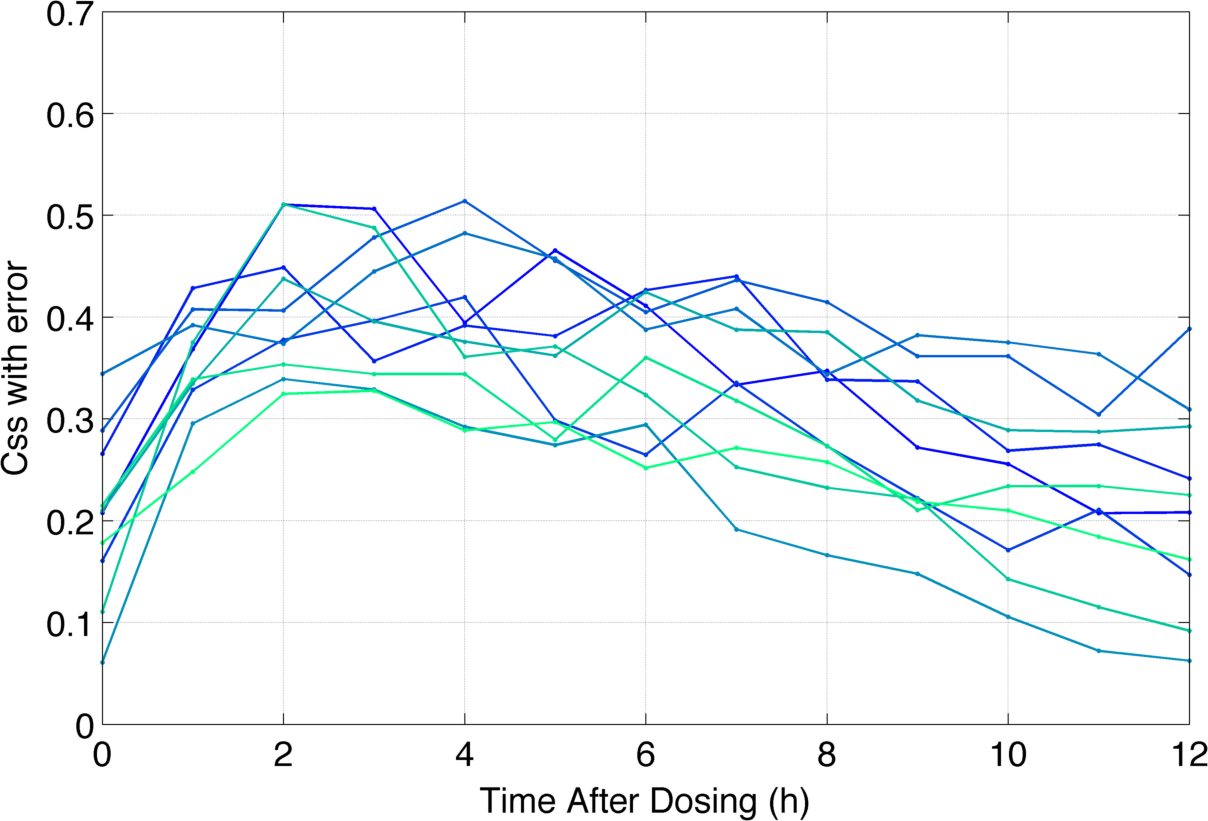
\includegraphics[width=.45\textwidth]{pics/Bonate_Css_proportionalError}
\caption{Simulated PK model as defined in the example for 10 subjects.}
\label{fig:BonatePK}
\vspace{-20pt}
\end{center}
\end{figure}
The only essential new aspect compared to the previous example is the fact
that we have here so called steady-state administration. For this to be defined
one needs to provide the time point of the last dosing event and the dose interval.

\subsection{Model Definition}
\subsubsection{Variability model}
The variability structure is identical to that in the previous example -- there is only
one level of subject related variability, see Figure \ref{fig:tree_IOV0}.

\subsubsection{Parameter model}

The model uses the following parameters:

\begin{align*}
\theta_{1,i} &=  \pop_{\theta_1} + \eta_{\theta_1,i}   \\
\log(V_i) &= \log(\pop_{V}) + \eta_{V,i}   \\
\theta_2 &= 0.75 \\
CL_i &= \theta_{1,i} \Big(\frac{W_i}{70}\Big)^{\theta_2} \\
K_a &= 0.5
\end{align*}
where
\begin{gather*}
\eta_{\theta_{1,i}} \sim N(0, \omega_{\theta_1}), \quad \eta_{V,i} \sim N(0,\omega_{V})
\intertext{and with}
\pop_{\theta_1}=25,\quad \omega_{\theta_1}=5  \quad \pop_V=250,\quad \omega_V=100.
\end{gather*}

\subsubsection{Covariate model}
%\begin{align*}
%\Covariates &: \Weight/70  \\
%\CovariatesType &: \Continuous  \\
%\CovariatesFile &: e.g. \textit{some\_filename.txt}  \\
%\Weight &\sim  \mbox{logNormal}(pop_{\Weight}, \omega_{\Weight}); \quad \pop_{\Weight}=80,\quad \omega_{\Weight}=9.6 
%\end{align*}

Body weight is the only covariate used in this model. It is used in the model
for the individual clearance only.
\begin{table}[h]
\begin{center}
\small
\renewcommand{\arraystretch}{1.1}% 
\begin{tabular}{lr}\toprule
 & \textbf{Weight} \\\midrule
Type & Continues \\
Transformation & $(\Weight/70)^{\theta_2}$ \\
Distribution & Normal \\
Mean, $pop_{\Weight}$ & 80 \\
Standard deviation, $\omega_{\Weight}$ & 9.6 \\
\bottomrule
\end{tabular}
\end{center}
\caption{Covariates overview.}
\label{tab:eg2-CovariatesOverview}
\end{table}


\subsubsection{Structural model}
\begin{align}
k &= \frac{CL}{V} \nonumber \\
C_{SS}(t) &= \frac{D}{V}\frac{K_a}{K_a - k} \bigg(\frac{e^{-k (t-t_D)}}{1-e^{-k \tau}}-\frac{e^{-K_a (t-t_D)}}{1-e^{-K_a\tau}}\bigg) \label{eqn:eg2-Css}
\end{align}

\subsubsection{Observation model}

We apply a residual error models to the output variable \var{C_{SS}}.

%\noindent
\begin{center}
\small
\renewcommand{\arraystretch}{1.1}% 
\begin{tabular*}{0.6\textwidth}{@{\extracolsep{\fill}} >{\bfseries}l l}\toprule
Output Variable  & \textbf{\itshape $C_{SS}$} \\\midrule
Observations Name & Concentration\\
Units & $\mg/l$ \\
Observations Type & Continuous \\
Residual Error Model & Proportional \\
Error Model Parameters & $b=0.1$\\
\bottomrule
\end{tabular*}
\end{center}

%%%%%%%%%%%%%%%%%%%%%%%%%%%%%%%%%%%%%%%%%%%%%%%%%%%%%%%%%%%%%%%%
\subsubsection{Trial design}

Table below summarises the information about the design in this example. 

%\noindent
\begin{center}
\small
\renewcommand{\arraystretch}{1.1}% 
\begin{tabular*}{0.45\textwidth}{@{\extracolsep{\fill}} >{\bfseries}l r}\toprule
Arm & \textbf{1} \\\midrule
Number of subjects & 50\\
Dose variable & \var{D} \\
Dosing Amount & 100 \\
Dose Units & $\mg$  \\
Dose per kg & no \\
Dosing times (h) & 0\\
Dose intervals (h) & 12\\
\bottomrule
\end{tabular*}
\end{center}

%%%%%%%%%%%%%%%%%%%%%%%%%%%%%%%%%%%%%%%%%%%%%%%%%%%%%%%%%%%%%%%%
\subsection{Simulation Step}
The concentration $C_{SS}$ is going to be read out at equidistant time points
after the dosing:
\begin{center}
\small
\renewcommand{\arraystretch}{1.1}% 
\begin{tabular*}{0.6\linewidth}{@{\extracolsep{\fill}} >{\bfseries}l c}\toprule
Output Variable & \textbf{\itshape $C_{SS}$}\\
\hline
Observation times & 0,1,2,3,4,5,6,7,8,9,10,11,12\\
\bottomrule
\end{tabular*}
\end{center}

\subsection{Structural model}
In the last example we defined the structural model by using an ODE system. 
Here, we implement an algebraic formula for the calculation of the drug
concentration in steady-state, \var{C_{SS}}, as shown in the following listing
%\inputxml{bonate_sm1_part1.xml}
\lstset{language=XML}
\begin{lstlisting}
            <ct:Variable symbolType="real" symbId="Css">
                <ct:Assign>
                    <Equation xmlns="http://www.pharmml.org/pharmml/0.6/Maths">
                        <Binop op="times">
                            <Binop op="divide">
                                <ct:SymbRef symbIdRef="D"/>
                                <ct:SymbRef blkIdRef="pm1" symbIdRef="V"/>
                            </Binop>
                            <Binop op="times">
                                <Binop op="divide">
                                    <ct:SymbRef blkIdRef="pm1" symbIdRef="Ka"/>
                                    <Binop op="minus">
                                        <ct:SymbRef blkIdRef="pm1" symbIdRef="Ka"/>
                                        <ct:SymbRef symbIdRef="k"/>
                                    </Binop>
                                </Binop>
                                <Binop op="minus">
                                    <Binop op="divide">
                                        <Uniop op="exp">
                                            <Binop op="times">
                                                <Uniop op="minus">
                                                    <ct:SymbRef symbIdRef="k"/>
                                                </Uniop>
                                                <Binop op="minus">
                                                    <ct:SymbRef symbIdRef="t"/>
                                                    <ct:SymbRef symbIdRef="tD"/>                                                    
                                                </Binop>
                                            </Binop>
                                        </Uniop>
                                        <Binop op="minus">
                                            <ct:Real>1</ct:Real>
                                            <Uniop op="exp">
                                                <Binop op="times">
                                                    <Uniop op="minus">
                                                        <ct:SymbRef symbIdRef="k"/>
                                                    </Uniop>
                                                    <ct:SymbRef blkIdRef="pm1" symbIdRef="tau"/>
                                                </Binop>
                                            </Uniop>
                                        </Binop>
                                    </Binop>
                                    <Binop op="divide">
                                        <Uniop op="exp">
                                            <Binop op="times">
                                                <Uniop op="minus">
                                                    <ct:SymbRef blkIdRef="pm1" symbIdRef="Ka"/>
                                                </Uniop>
                                                <Binop op="minus">
                                                    <ct:SymbRef symbIdRef="t"/>
                                                    <ct:SymbRef symbIdRef="tD"/>                                                    
                                                </Binop>
                                            </Binop>
                                        </Uniop>
                                        <Binop op="minus">
                                            <ct:Real>1</ct:Real>
                                            <Uniop op="exp">
                                                <Binop op="times">
                                                    <Uniop op="minus">
                                                        <ct:SymbRef blkIdRef="pm1" symbIdRef="Ka"/>
                                                    </Uniop>
                                                    <ct:SymbRef blkIdRef="pm1" symbIdRef="tau"/>
                                                </Binop>
                                            </Uniop>
                                        </Binop>
                                    </Binop>
                                </Binop>
                            </Binop>
                        </Binop>
                    </Equation>
                </ct:Assign>
            </ct:Variable>
\end{lstlisting}

Consequently, we use for \var{C_{SS}} the \xelem{Variable}, instead of \xelem{DerivativeVariable},
element as in the previous example which is of \xatt{real} type.

\subsection{Trial design model}
\subsubsection{Structure}

Figure \ref{fig:designPatternBonate} shows the \textit{Structure} of
this simple example consisting of 1 arm and one epoch, meaning one treatment
type for everybody.

\begin{figure}[ht!]
\centering
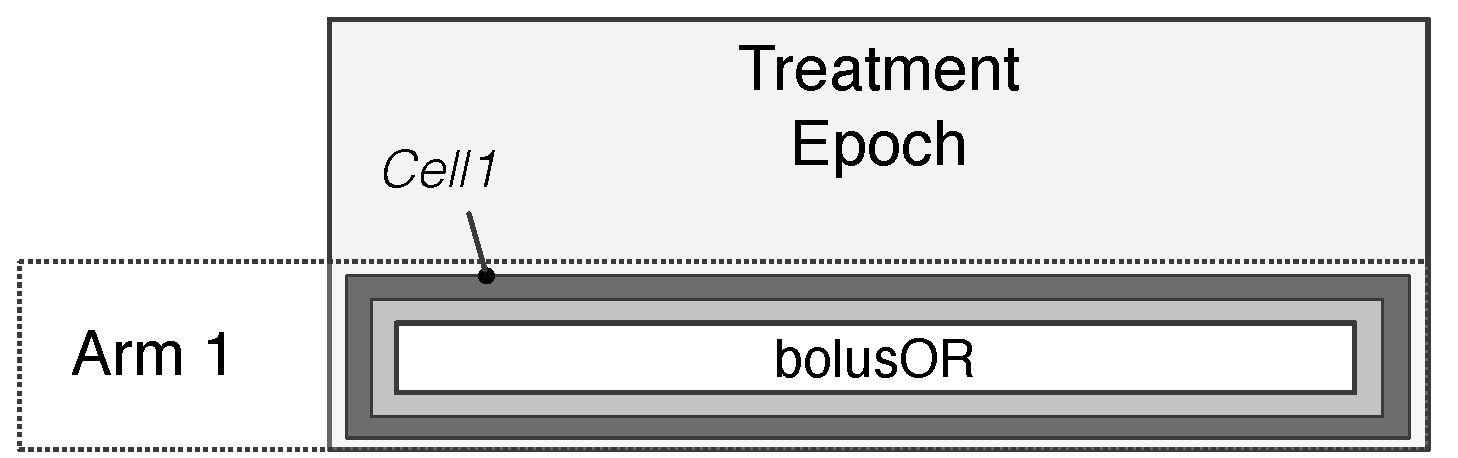
\includegraphics[width=0.7\linewidth]{pics/OneArmOneEpoch}
\caption{Design overview: this study consists of one arm and one epoch.}
\label{fig:designPatternBonate}
\end{figure}

\begin{table}[htdp!]
\begin{center}
\renewcommand{\arraystretch}{1.1}% 
\begin{tabular}{ccccccc}
\hline
Segment&Activity & Treatment & DoseTime & DoseSize & Target Variable \\
\hline
TA& bolusOR &  OR bolus & 0 & 100 & D \\
\hline
\end{tabular}
\end{center}
\caption{Segment/activity overview.}
%\label{tab:segementActivity_Ribba}
\end{table}

\begin{table}[htdp!]
\begin{center}
\renewcommand{\arraystretch}{1.1}% 
\begin{tabular}{ccc}
\hline
Epoch & Start time & End time \\
\hline
Treatment Epoch & 0 &  12  \\
\hline
\end{tabular}
\end{center}
\caption{Epoch definition -- there is only one epoch here.}
\label{fig:Bonate:epochDef}
\end{table}

While the implementation of epoch, arm, cell and segment is analog to that in the 
previous example, the \xelem{Activity} element contains new items. After we 
defined \xelem{DoseAmount} as before as well, the steady-state administration 
is easily implemented using the \xelem{SteadyState} with last doing event as
\xelem{EndTime} and the dose interval as \xelem{Interval} as can be seen 
in the following listing 
%\inputxml{bonate_activity.xml}
\lstset{language=XML}
\begin{lstlisting}
            <Activity oid="bolusOR">
                <Bolus>
                    <DoseAmount inputTarget="parameter">
                        <ct:SymbRef blkIdRef="sm1" symbIdRef="D"/>
                        <ct:Assign>
                            <ct:Real>100</ct:Real>
                        </ct:Assign>
                    </DoseAmount>
                    <SteadyState>
                        <EndTime>
                            <ct:SymbRef blkIdRef="sm1" symbIdRef="tD"/>
                            <ct:Assign>
                                <ct:Real>0</ct:Real>
                            </ct:Assign>
                        </EndTime>
                        <Interval>
                            <ct:SymbRef blkIdRef="pm1" symbIdRef="tau"/>
                            <ct:Assign>
                                <ct:Real>12</ct:Real>
                            </ct:Assign>
                        </Interval>
                    </SteadyState>
                </Bolus>
            </Activity>
\end{lstlisting}


%%%%%%%%%%%%%%%%%%%%%%%%%%%%%%%%%%%%%%%%%%%%%%%%%%%%%%%%%%%%%%%%
\subsection{NONMEM dataset}
\label{sec:eg2-NONMEMdataset}
Table \ref{tab:example2_dataSet} shows the typical NONMEM dataset 
to be used with this model for few selected subject. The subsequent
listing shows then its definition and mappings  


\begin{table}[htdp]
\begin{center}
\small
\renewcommand{\arraystretch}{1.1}% 
\begin{tabular}{rrrrrrr}\toprule
ID	& TIME 	& WT	& DV		& EVID	& MDV \\\midrule
1	& 0		& 82		& 		& 0		& 0	\\
1	& 1		& 82		& 		& 0		& 0	\\
1	& 2		& 82		& 		& 0		& 0	\\
...	& ...		& ...		& ...		& ...		& ...	\\
1	& 11		& 82		& 		& 0		& 0	\\
1	& 12		& 82		& 		& 0		& 0	\\
2	& 0		& 77		& 		& 0		& 0	\\
2	& 1		& 77		& 		& 0		& 0	\\
2	& 2		& 77		& 		& 0		& 0	\\
...	& ...		& ...		& ...		& ...		& ...	\\
2	& 11		& 77		& 		& 0		& 0	\\
2	& 12		& 77		& 		& 0		& 0	\\
3	& 0		& 94		& 		& 0		& 0	\\
...	& ...		& ...		&...		& ...		& ...	\\ \bottomrule
\end{tabular}
\end{center}
\caption{A dataset used in example \theexamples. WT data has to be provided 
as sampled from normal distribution as specified in Table \ref{tab:eg2-CovariatesOverview}.}
\label{tab:example2_dataSet}
\end{table}%
\lstset{language=XML}
\begin{lstlisting}
        <ExternalDataSet toolName="NONMEM" oid="NMoid">
            
            <ColumnMapping>
                <ColumnRef xmlns="http://www.pharmml.org/pharmml/0.6/Dataset" columnIdRef="ID"/>
                <ct:SymbRef blkIdRef="vm1" symbIdRef="indiv"/>
            </ColumnMapping>
            <ColumnMapping>
                <ColumnRef xmlns="http://www.pharmml.org/pharmml/0.6/Dataset" columnIdRef="TIME"/>
                <ct:SymbRef symbIdRef="t"/>
            </ColumnMapping>
            <ColumnMapping>
                <ColumnRef xmlns="http://www.pharmml.org/pharmml/0.6/Dataset" columnIdRef="WT"/>
                <ct:SymbRef blkIdRef="cm1" symbIdRef="Weight"/>
            </ColumnMapping>            
            <ColumnMapping>
                <ColumnRef xmlns="http://www.pharmml.org/pharmml/0.6/Dataset" columnIdRef="DV"/>
                <ct:SymbRef blkIdRef="om1" symbIdRef="Css_obs"/>
            </ColumnMapping>
            
            <DataSet xmlns="http://www.pharmml.org/pharmml/0.6/Dataset">
                <Definition>
                    <Column columnId="ID" columnType="id" valueType="string" columnNum="1"/>
                    <Column columnId="TIME" columnType="idv" valueType="real" columnNum="2"/>
                    <Column columnId="WT" columnType="covariate" valueType="real" columnNum="3"/>
                    <Column columnId="DV" columnType="dv" valueType="real" columnNum="4"/>
                    <Column columnId="EVID" columnType="evid" valueType="int" columnNum="5"/>
                    <Column columnId="MDV" columnType="mdv" valueType="int" columnNum="6"/>
                </Definition>
                <ImportData oid="dataOid">
                    <path>example2.csv</path>
                    <format>CSV</format>
                    <delimiter>COMMA</delimiter>
                </ImportData>
            </DataSet>
        </ExternalDataSet>
\end{lstlisting}
        
Note, that the sampling distribution defined in the covariate model
cannot be used, this applies to situations when e.g. NONMEM is the target tool, 
and the dataset needs to provide the sampled normal distributed weight values for each 
subject. This is why the column $WT$ is in the dataset, Table \ref{tab:example2_dataSet}. 
This continues covariate is mapped to the 
\xelem{CovariateModel} which shorter then the one before and contains 
only the allometric transformation as the following snippet shows
\lstset{language=XML}
\begin{lstlisting}
        <CovariateModel blkId="cm1">
            <Covariate symbId="Weight">
                <Continuous>
                    <Transformation>
                        <TransformedCovariate symbId="theta2Weight"/>
                        <Equation xmlns="http://www.pharmml.org/pharmml/0.6/Maths">
                            <Binop op="power">
                                <Binop op="divide">
                                    <ct:SymbRef symbIdRef="Weight"/>
                                    <ct:Real>70</ct:Real>
                                </Binop>
                                <ct:SymbRef blkIdRef="pm1" symbIdRef="theta2"/>
                            </Binop>
                        </Equation>
                    </Transformation>
                </Continuous>
            </Covariate>
        </CovariateModel>
\end{lstlisting}

Here the dose or dosing time are not stored in the dataset, they can be defined
and assigned in the \xelem{StructuralModel} and \xelem{SimulationStep}, respectively
This corresponds to the situation when these data together with the structural model
are implemented in the \emph{\$PRED} section in NMTRAN.


%%%%%%%%%%%%%%%%%%%%%%%%%%%%%%%%%%%%%%%%%%%%%%%%%%%%%%%%%%%%%%%%
%%%%%%%%%%%%%%%%%%%%%%%%%%%%%%%%%%%%%%%%%%%%%%%%%%%%%%%%%%%%%%%%
%%%%%%%%%%%%%%%%%%%%%%%%%%%%%%%%%%%%%%%%%%%%%%%%%%%%%%%%%%%%%%%%
\eglabel{3}
\section{Example \theexamples: Estimation, Warfarin PK}
\label{sec:eg3}

\subsection{Description}

This model describes the PK of warfarin\footnote{The example is encoded in two versions,  
\xatt{example3.xml} and \xatt{example3\_NONMEM.xml}, with explicit encoded trial 
design and design sourced from a NONMEM datafile, respectively.}.
 
% and corresponds to the \ddmore WP3 use case 
% Warfarin\_PK\_PRED\footnote{\raggedright Available via Interface Europe:
% \url{https://cp1.interfaceurope.eu/LotusQuickr/ddmore/PageLibraryC125786900388659.nsf/h_Toc/92be13faec1b58390525670800167238/?OpenDocument\#{type=0\&unid=5801C48FC6C39BB141257B2A007D6F31}}}. 

\subsubsection{Structural model}

The model is a one compartment model with first-order absorption with
lag time and first-order elimination.

\begin{description}
\item[\itshape D] Dosing variable.
\item[\itshape t\textsubscript{D}] Time of the dose.
\item[\itshape C] Concentration of drug in the compartment.
\end{description}
\begin{align*}
k &= \frac{\CL}{V}\\
C(t) &= \begin{cases}
  0 & \text{if } \quad t - t_D < \Tlag \\
  \frac{D}{V}\frac{k_a}{k_a-k}\left[e^{-k\,
       \left(t-t_D-T_{lag}\right)}-e^{-k_a \, \left(t-t_D-T_{lag}\right)}\right] &
  \text{otherwise}
\end{cases}
\end{align*}


\subsubsection{Covariate model}

Body weight, $W$, is the only continue covariate used in this model. It is used in the model
for the individual clearance and volume.
\begin{table}[h]
\begin{center}
\renewcommand{\arraystretch}{1.1}% 
\begin{tabular}{lr}\toprule
 & \textbf{Weight} \\\midrule
Type & Continues \\
Transformation & $\log(\Weight/70)$ \\
\bottomrule
\end{tabular}
\end{center}
\caption{Covariates overview.}
\label{tab:CovariatesOverview}
\end{table}


\subsubsection{Parameters}

\paragraph{PK Parameters}

The following PK parameters are used in the model:
\begin{description}
\item[\Tlag] The lag time.
\item[\ka] The absorption rate constant.
\item[\var{V}] The volume of distribution.
\item[\CL] Clearance of elimination.
\end{description}

\begin{align*}
\intertext{The parameters are defined as follows:}
\log(\Tlag) &= \log(pop\_\Tlag) + \eta_\Tlag\\
\log(\ka) &= \log(pop\_\ka) + \eta_\ka\\
\log(\var{V}) &= \log(pop\_\var{V}) + \beta_{1,V} \log(W_i/70) + \eta_\var{V}\\
\log(\CL) &= \log(pop\_\CL) + \beta_{1,\CL} \log(W_i/70) + \eta_\CL
\end{align*}
where
\begin{gather*}
\eta_\Tlag \sim \mathcal{N}(0, \omega_{\Tlag}), \quad \eta_\ka \sim \mathcal{N}(0, \omega_{\ka}),\\
\eta_\var{V} \sim  \mathcal{N}(0, \omega_{V}), \quad \eta_\CL \sim \mathcal{N}(0, \omega_{\CL})
\end{gather*}
Note please that, in this case, $\beta_{1,V}=0.75$ and $\beta_{1,CL}=1$, i.e. are fixed and will not be estimated.

\paragraph{Variance-covariance matrix}
The full variance-covariance matrix for the random effects is :
\begin{equation*}
 \Omega =
 \begin{pmatrix}
  \omega_{Tlag}^2 	& 0 				& 0                                 & 0  \\
   			  	& \omega_{\ka}^2	& 0                                 & 0  \\
  				& 				& \omega_{\var{V}}^2     & 0  \\
 				&				&                                    & \omega_{\CL}^2 \\
 \end{pmatrix}
%\label{sec:eg-covariance-mat}
\end{equation*}

\subsubsection{Observation model}

We apply a residual error models to the output variable \var{C}.

%\noindent
\begin{center}
\small
\renewcommand{\arraystretch}{1.1}% 
\begin{tabular*}{0.6\textwidth}{@{\extracolsep{\fill}} >{\bfseries}l l}\toprule
Output Variable  & \textbf{\itshape C} \\\midrule
Observations Name & Concentration\\
Units & $\mg/l$ \\
Observations Type & Continuous \\
Residual Error Model & Combined2 \\
Error Model Parameters & $a = 0.1,\quad b=0.1$\\
\bottomrule
\end{tabular*}
\end{center}

\subsubsection{Trial Design}
\label{sec:eg4-trial-design}

The dosing regimen for the trial is given below --- there is only one
for each arm. Note that all dosing is bolus dosing (discrete
administration at specific times) and all doses are administered to
the same compartment.

%\noindent
\begin{center}
\small
\renewcommand{\arraystretch}{1.1}% 
\begin{tabular*}{0.45\textwidth}{@{\extracolsep{\fill}} >{\bfseries}l r}\toprule
Arm & \textbf{1} \\\midrule
Number of subjects & 33\\
Dose variable & \var{D} \\
Dosing Amount & 100 \\
Dose Units & $\mg$  \\
Dose per kg & no \\
Dosing times (h) & 0\\
\bottomrule
\end{tabular*}
\end{center}

% The trial is has just one study group of 33 individuals.
% \begin{align*}
% \DoseTime (t_D)&= 0    \\
% \TimeUnit&= h
% \intertext{Dosing is adjusted to body weight}
% \DoseSize&= 100  \\
% \DosePerKg&=\no   \\
% \DoseUnit&=\mg
% \intertext{Time of measurement for PK}
% \ObservationTime&= 0.5,1,2,3,6,9,24,36,48,72,96,120
% \end{align*}

\subsubsection{Modelling Steps}

The observations for the output variable is shown below. These
time-points correspond to those define in the data-file. The task to
be performed is a parameter estimation which will involved the
following steps:
\begin{itemize}
\item Estimation of population paramaters.
\item Estimation of Fisher information matrix.
\item Estimation of the individual parameters.
\end{itemize}

%\noindent
\begin{center}
\begin{tabular*}{0.6\linewidth}{@{\extracolsep{\fill}} >{\bfseries}l c}\toprule
Output Variable & \textbf{\itshape C}\\
\hline
Observation times & 0.5,1,2,3,6,9,24,36,48,72,96,120\\
\bottomrule
\end{tabular*}
\end{center}

\begin{figure}[ht!]
\centering
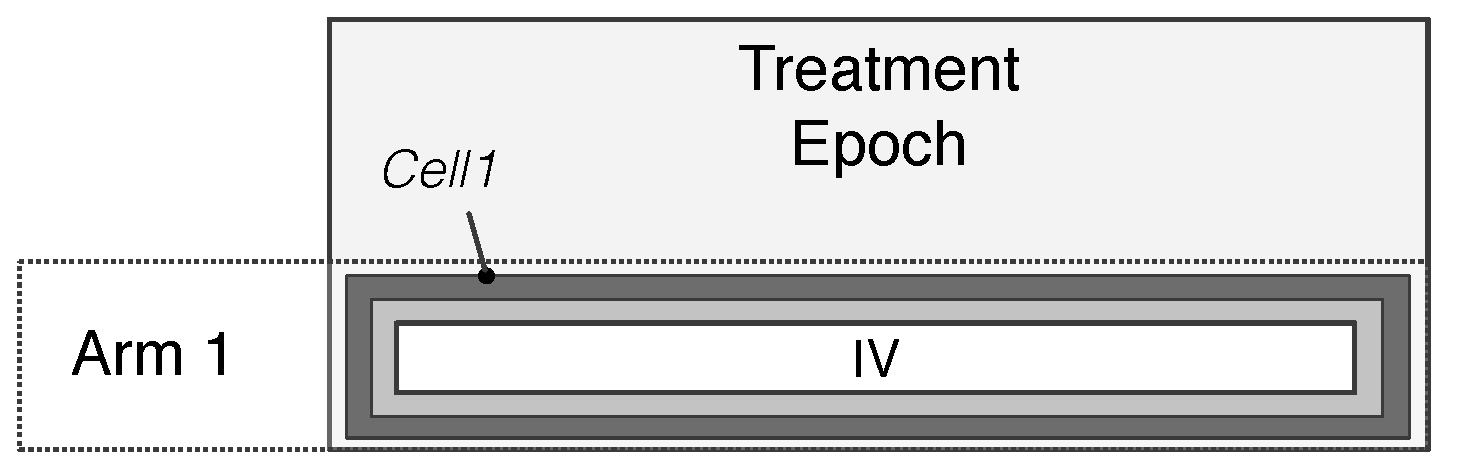
\includegraphics[width=0.7\linewidth]{pics/OneArmOneEpoch_IV}
\caption{Design overview: this study consists of one arm and one epoch.}
\label{fig:designPattern_1Arm1Epoch}
\end{figure}

Figure \ref{fig:designPattern_1Arm1Epoch} shows the \textit{Structure} of
this simple example consisting of 1 arm and one epoch, meaning one treatment
type for everybody.

%
% The output variable is:
% \begin{description}
% \item[\var{C}] Concentration in the central compartment, in this case
%     the bloodstream.
% \end{description}

\subsection{Overview}

This our first estimation case. From figure \ref{fig:EstimationTask_List} 
it follows that we can expect significant differences in the Trial Design and Modelling Steps
sections compared to the previous simulation case.

%, see listing \ref{fig:exp5_modelOverview}
%for an overview.

Accordingly, the Model Definition is very similar to that in the
previous example.  The main \pharmml feature we have not seen
previously is the algebraic structural model (i.e., the model is not
defined as a system of ODEs). The XML is too long to show here and is
similar to the examples shown previously (section \ref{sec:maths}). If
you are interested then please consult the full example associated
with this specification.

We will start with the description of the Trail design. Note that because
every subject receives the same dosing regimen, this can be encoded 
in the \xelem{Activity} block. Otherwise we would have to define the 
individual dosing regimens in the \xelem{IndividualDosing} element, see
section \ref{subsubsec:Ribba_indivDosing} in example \ref{sec:Ribba} how
this is done.

%\begin{listing}[htb]
%\inputxml{exp5_modelOverview.xml}
%\caption{Defining the complete model.}
%\label{fig:exp5_modelOverview}
%\end{listing}


\subsection{Trial Design}
\label{eg4_subsec:trialDesign}
\subsubsection{Structure}

As explained in the chapter \ref{sec:CTS} on trial design, we base the following 
structure on the CDISC standard Study Design Model \cite{CDISC:2011a}. 
The design elements are contained in the \xelem{Structure} block and you can see 
in following listing 
%\inputxml{exp5_structure.xml}
\lstset{language=XML}
\begin{lstlisting}
        <Structure>
            <Epoch oid="epoch1">
                <Start><ct:Real>0</ct:Real></Start>
                <End><ct:Real>180</ct:Real></End>
                <Order>1</Order>
            </Epoch>
            <Arm oid="arm1"/>
            <Cell oid="cell1">
                <EpochRef oidRef="epoch1"/>
                <ArmRef oidRef="arm1"/>
                <SegmentRef oidRef="segment1"/>
            </Cell>
            <Segment oid="segment1">
                <ActivityRef oidRef="d1"/>
            </Segment>
            <Activity oid="d1">
                <Bolus>
                    <DoseAmount inputTarget="parameter">
                        <ct:SymbRef blkIdRef="sm1" symbIdRef="D"/>
                        <ct:Assign>
                            <ct:Real>100</ct:Real>
                        </ct:Assign>
                    </DoseAmount>
                    <DosingTimes>
                        <ct:SymbRef blkIdRef="sm1" symbIdRef="tD"/>
                        <ct:Assign>
                            <ct:Real>0</ct:Real>
                        </ct:Assign>
                    </DosingTimes>
                </Bolus>
            </Activity>
        </Structure>
\end{lstlisting}

how the study is constructed of a single epoch, 
with a single arm and a single cell that contains a single segment. Note, though 
that this structure is not hierarchical and the \xelem{Cell} element joins the arm, 
epoch and segments together. 

The last section of the structure, the \xelem{Activity} element, is of interest for 
the discussion. This is because, as already mentioned above, the administration
and dosing regimen is identical for every patient. The dose amount is $D=100\; mg$ 
and the dose time is $t_D=0$.
As in the previous example, the structural model is defined using an algebraic
function with the dosing variable \var{D} which means the \xelem{DoseAmount} element
has the attribute \xatt{inputType="parameter"}. Additionally the dosing time variable \var{tD} is
referenced here and initialised. 


%\begin{listing}[htb]
%\inputxml{exp5_structure.xml}
%\caption{Structure overview.}
%\label{lst:exp5_structure}
%\end{listing}

\subsubsection{Population}

This is the place where we describe the individuals in the study, which 
\var{Arm} they belong to and any possible individual characteristics, such as 
body weight, age and other covariates. In this example we only know the
body weight of the subjects. 
We define the known attributes of all individuals using the 
\xelem{IndividualTemplate} and then map each individual to this template 
using a \xelem{Dataset}. In the following listing 
%\inputxml{exp5_population.xml}
\lstset{language=XML}
\begin{lstlisting}
        <Population>
            <ColumnMapping>
                <ds:ColumnRef columnIdRef="WEIGHT"/>
                <ct:SymbRef blkIdRef="cm1" symbIdRef="W"/>
            </ColumnMapping>
            
            <ds:DataSet>
                <ds:Definition>
                    <ds:Column columnId="ID" columnType="id" valueType="string" columnNum="1"/>
                    <ds:Column columnId="ARM" columnType="arm" valueType="id" columnNum="2"/>
                    <ds:Column columnId="WEIGHT" columnType="covariate" valueType="real" columnNum="3"/>
                </ds:Definition>
                <ds:Table>
                    <ds:Row><ct:String>1</ct:String><ct:Id>arm1</ct:Id><ct:Real>70.1</ct:Real></ds:Row>
                    <ds:Row><ct:String>2</ct:String><ct:Id>arm1</ct:Id><ct:Real>60.0</ct:Real></ds:Row>
                    <ds:Row><ct:String>3</ct:String><ct:Id>arm1</ct:Id><ct:Real>93.2</ct:Real></ds:Row>
                    <ds:Row><ct:String>4</ct:String><ct:Id>arm1</ct:Id><ct:Real>85.7</ct:Real></ds:Row>
                    <ds:Row><ct:String>5</ct:String><ct:Id>arm1</ct:Id><ct:Real>78.3</ct:Real></ds:Row>
                    <!-- SNIP -->
                    <ds:Row><ct:String>33</ct:String><ct:Id>arm1</ct:Id><ct:Real>94.1</ct:Real></ds:Row>
                </ds:Table>
            </ds:DataSet>
        </Population>
\end{lstlisting}

you can see how this 
is implemented in \pharmml. Column \var{2} in the table is equal for
every subject because they all belong to one arm, here denoted as \var{a1}.



%%%%%%%%%%%%%%%%%%%%%%%%%%%%%%%%%%%%%%%%%%%%%%%%%%%%%%%%%%%%%%%%
\subsection{NONMEM dataset}
\label{sec:eg3-NONMEMdataset}
Now we will describe the case when the data and trial design are sourced from the 
NONMEM dataset. Table \ref{tab:example3_dataSet} show a typical dataset required for 
an estimation task.
\begin{table}[htdp]
\begin{center}
\small
\renewcommand{\arraystretch}{1.1}% 
\begin{tabular}{rrrrrrrrr}\toprule
ID	& TIME	& WT	& AMT	& DVID	& DV		& MDV  \\\midrule
1	& 0		& 66.7	& 100	& 0		& .		& 1  \\
1	& 0.5	& 66.7	& .		& 1		& 0		& 0  \\
1	& 1		& 66.7	& .		& 1		& 1.9	& 0  \\
1	& 2		& 66.7	& .		& 1		& 3.3	& 0  \\
1	& 3		& 66.7	& .		& 1		& 6.6	& 0  \\
...	& ...		& ...		&...		& ...		& ...		& ... \\
1	& 120	& 66.7	& .		& 1		& 0.8	& 0  \\
2	& 0		& 80 	& 100	& 0		& .		& 1 \\
2	& 0.5	& 80 	& .		& 1		& 9.2	& 0 \\
2	& 1		& 80		& .		& 1		& 8.5	& 0 \\
2	& 2		& 80		& .		& 1		& 6.4	& 0 \\
2	& 3		& 80		& .		& 1		& 4.8	& 0 \\
...	& ...		& ...		& ...		& ...		& ...		& ... \\ \bottomrule
\end{tabular}
\end{center}
\caption{A fragment of the dataset used in example \theexamples\; for two first subjects.}
\label{tab:example3_dataSet}
\end{table}%

The following code shows how the dataset definition and column mappings 
are done
\lstset{language=XML}
\begin{lstlisting}
        <ExternalDataSet toolName="NONMEM" oid="NMoid">
            
            <ColumnMapping>
                <ds:ColumnRef columnIdRef="ID"/>
                <ct:SymbRef blkIdRef="vm1" symbIdRef="indiv"/>
            </ColumnMapping>
            <ColumnMapping>
                <ds:ColumnRef columnIdRef="TIME"/>
                <ct:SymbRef symbIdRef="t"/>
            </ColumnMapping>
            <ColumnMapping>
                <ds:ColumnRef columnIdRef="WT"/>
                <ct:SymbRef blkIdRef="cm1" symbIdRef="W"/>
            </ColumnMapping>
            <ColumnMapping>
                <ds:ColumnRef columnIdRef="DV"/>
                <ct:SymbRef blkIdRef="om1" symbIdRef="C_obs"/>
            </ColumnMapping>
            <ColumnMapping>
                <ColumnRef xmlns="http://www.pharmml.org/pharmml/0.6/Dataset" columnIdRef="AMT"/>
                <ct:SymbRef blkIdRef="sm1" symbIdRef="D"/>
            </ColumnMapping>
            <ColumnMapping>
                <ColumnRef xmlns="http://www.pharmml.org/pharmml/0.6/Dataset" columnIdRef="TIME"/>
                <Piecewise xmlns="http://www.pharmml.org/pharmml/0.6/Dataset">
                    <math:Piece>
                        <ct:SymbRef blkIdRef="sm1" symbIdRef="tD"/>
                        <math:Condition>
                            <math:LogicBinop op="neq">
                                <ColumnRef columnIdRef="AMT"/>
                                <ct:Real>0</ct:Real>
                            </math:LogicBinop>
                        </math:Condition>
                    </math:Piece>
                </Piecewise>
            </ColumnMapping>
            <ds:DataSet>
                <ds:Definition>
                    <ds:Column columnId="ID" columnType="id" valueType="string" columnNum="1"/>
                    <ds:Column columnId="TIME" columnType="time" valueType="real" columnNum="2"/>
                    <ds:Column columnId="WT" columnType="covariate" valueType="real" columnNum="3"/>
                    <ds:Column columnId="AMT" columnType="dose" valueType="real" columnNum="4"/>
                    <ds:Column columnId="DVID" columnType="dvid" valueType="real" columnNum="5"/>
                    <ds:Column columnId="DV" columnType="dv" valueType="real" columnNum="6"/>
                    <ds:Column columnId="MDV" columnType="mdv" valueType="real" columnNum="7"/>
                </ds:Definition>
                <ds:ImportData oid="dataOid">
                    <ds:path>example3.csv</ds:path>
                    <ds:format>CSV</ds:format>
                    <ds:delimiter>COMMA</ds:delimiter>
                </ds:ImportData>
            </ds:DataSet>
        </ExternalDataSet>
\end{lstlisting}

Contrary to the previous example, we store now the dosing data in the dataset
and therefore require to provide the additioanl column mapping. The column AMT
is mapped in the usual fashion to its target, the dose variable, $D$. 
The mapping of the dosing time variable, $tD$, is a bit more interesting as it requires 
a mapping of the $TIME$ column to variable $tD$ only when the actual doing happens. This is
the case when the $AMT \neq 0$. Which is what is encoded in the last 
\xelem{ColumnMapping} of the listing above using the \xelem{Piecewise} element.



%%%%%%%%%%%%%%%%%%%%%%%%%%%%%%%%%%%%%%%%%%%%%%%%%%%%%%%%%%%%%%%%
\subsection{Modelling Steps}

\subsubsection{Objective data}
Remember that according to Figure \ref{fig:EstimationTask_List} this element
is required only when working with explicit trial design.

An advantage of PharmML is that we do not have
to define the design in the data file. Instead of using NONMEM dataset as 
demonstrated in the previous section and after the structure of the trial is defined
as above, see Section \ref{eg4_subsec:trialDesign}, we just need to encode the 
measured experimental data, here the time and the independent variable, the 
concentration values. To achieve that we define a table in \xelem{Dataset} with 
columns: \var{ID}, \var{time} and \var{dv} and populate it with given experimental 
values, see \xelem{ObjectiveDataSet} block in the following listing 
%\inputxml{exp5_objDataSet.xml}
\lstset{language=XML}
\begin{lstlisting}
    <ObjectiveDataSet>
        <ColumnMapping>
            <ds:ColumnRef columnIdRef="time"/>
            <ct:SymbRef symbIdRef="t"/>
        </ColumnMapping>
        <ColumnMapping>
            <ds:ColumnRef columnIdRef="dv"/>
            <ct:SymbRef blkIdRef="om1" symbIdRef="C_obs"/>
        </ColumnMapping>
        <ds:DataSet>
            <ds:Definition>
                <ds:Column columnId="ID" columnType="id" valueType="string" columnNum="1"/>
                <ds:Column columnId="time" columnType="time" valueType="real" columnNum="2"/>
                <ds:Column columnId="dv" columnType="dv" valueType="real" columnNum="3"/>
            </ds:Definition>
            <ds:Table>
                <!-- SUBJECT 1 -->
                <ds:Row><ct:String>1</ct:String><ct:Real>0.5</ct:Real><ct:Real>0</ct:Real></ds:Row>
                <ds:Row><ct:String>1</ct:String><ct:Real>1</ct:Real><ct:Real>1.9</ct:Real></ds:Row>
                <ds:Row><ct:String>1</ct:String><ct:Real>2</ct:Real><ct:Real>3.3</ct:Real></ds:Row>
                <ds:Row><ct:String>1</ct:String><ct:Real>3</ct:Real><ct:Real>6.6</ct:Real></ds:Row>
                <ds:Row><ct:String>1</ct:String><ct:Real>6</ct:Real><ct:Real>9.1</ct:Real></ds:Row>
                <ds:Row><ct:String>1</ct:String><ct:Real>9</ct:Real><ct:Real>10.8</ct:Real></ds:Row>
                <!-- SUBJECT 2 -->
                <!-- SNIP -->
            </ds:Table>
        </ds:DataSet>
    </ObjectiveDataSet>
\end{lstlisting}

Similarly to the situation before we have to make sure that these values are 
correctly mapped to variable used in the model which is implemented in the 
\xelem{ColumnMapping} element. The ID column doesn't have to be mapped, 
the attribute \xatt{columnType="id"}, the \emph{subject identifiers}, assigns the 
proper meaning to this symbol, see Table \ref{tab:MDLPharmML_columnTypes}. 
Here the \var{time} as in the data is mapped 
to model time \var{t} and the measured concentration is mapped to the 
variable $C_{obs}$ as in the observation model.


%\begin{listing}[htb]
%\inputxml{exp5_objDataSet.xml}
%\caption{Objective dataset overview.}
%\label{fig:exp5_objDataSet}
%\end{listing}	

\subsubsection{Parameter estimation}


In a parameter estimation you do not necessarily want to estimate all
the parameters in your model or you may wish to define bounds within
which your parameter should be estimated, or provide an initial
estimate.  The \xelem{ParametersToEstimate} element controls this. As
you can see in the following listing 
%\inputxml{exp5_paramEstimation.xml}
\lstset{language=XML}
\begin{lstlisting}
                <ParameterEstimation>
                    <ct:SymbRef blkIdRef="pm1" symbIdRef="pop_V"/>
                    <InitialEstimate fixed="false">
                        <ct:Real>10</ct:Real>
                    </InitialEstimate>
                </ParameterEstimation>
                <ParameterEstimation>
                    <ct:SymbRef blkIdRef="pm1" symbIdRef="omega_V"/>
                    <InitialEstimate fixed="false">
                        <ct:Real>1</ct:Real>
                    </InitialEstimate>
                </ParameterEstimation>
\end{lstlisting}

we use a \xelem{ParameterEstimation} element that refers to the parameter in
the model definition.  In its simplest form you can decide whether the
parameter is to be estimated by setting the \xatt{fixed} attribute
(false indicates the parameter should be estimated). If a parameter is
not defined here, then it is assumed that it will not be estimated, in
which case it would be assigned an initial value elsewhere in the
PharmML document.  One of the validation rules (see chapter
\ref{chapter:validation}) is that every parameter has to be
initialised. 
%This can happen either in the \xelem{ParameterModel},
%\xelem{ObservationModel} or in this \xelem{ParametersToEstimate} block.
 

%\subsubsection{Operation}
%
%\begin{listing}[htb]
%\inputxml{exp5_operation.xml}
%\caption{Operation overview.}
%\label{fig:exp5_operation}
%\end{listing}


\subsubsection{Step dependencies}

Then at the end of the \xelem{ModellingSteps} block is the \xelem{StepDependencies} element. 
This describes the ordering of the steps in the modelling process, but in this case it is 
almost trivial as we only have one step in this example:
%\inputxml{exp5_steps.xml}
\lstset{language=XML}
\begin{lstlisting}
        <mstep:StepDependencies>
            <mstep:Step>
                <ct:OidRef oidRef="estimStep1"/>
            </mstep:Step>
        </mstep:StepDependencies>
\end{lstlisting}


%%%%%%%%%%%%%%%%%%%%%%%%%%%%%%%%%%%%%%%%%%%%%%%%%%%%%%%%%%%%%%%%
%%%%%%%%%%%%%%%%%%%%%%%%%%%%%%%%%%%%%%%%%%%%%%%%%%%%%%%%%%%%%%%%
%%%%%%%%%%%%%%%%%%%%%%%%%%%%%%%%%%%%%%%%%%%%%%%%%%%%%%%%%%%%%%%%
\eglabel{4}
\section{Example \theexamples: Estimation with IOV}
\label{sec:eg4}

%%%%%%%%%%%%%%%%%%%%%%%%%%%%%%%%%%%%%%%%%%%%%%%%%%%%%%%%%%%%%%%%
\subsection{Description}

In this example we will look at a more complex trial design and a
correspondingly complex variability model\footnote{The example is 
encoded in two versions, \xatt{example4.xml} and \xatt{example4\_NONMEM.xml}, 
with explicit encoded trial design and design sourced from a NONMEM datafile, 
respectively.}. The model also includes categorical covariates, which is again 
something we have not encountered thus far. The example is based on 
example IOV1 from Monolix 4.1 (see \cite{Monolix4.1.4UserGuide:2012} for a detailed
description) and features a cross-over design and inter-occasion
variability (see section \ref{sec:variabilityModel}). As before we will
go through the key elements of the model before we look at the
\pharmml examples, but given the complex nature of the trial design we
will describe that first then move onto the model definition.


\begin{figure}[htb]
\centering
 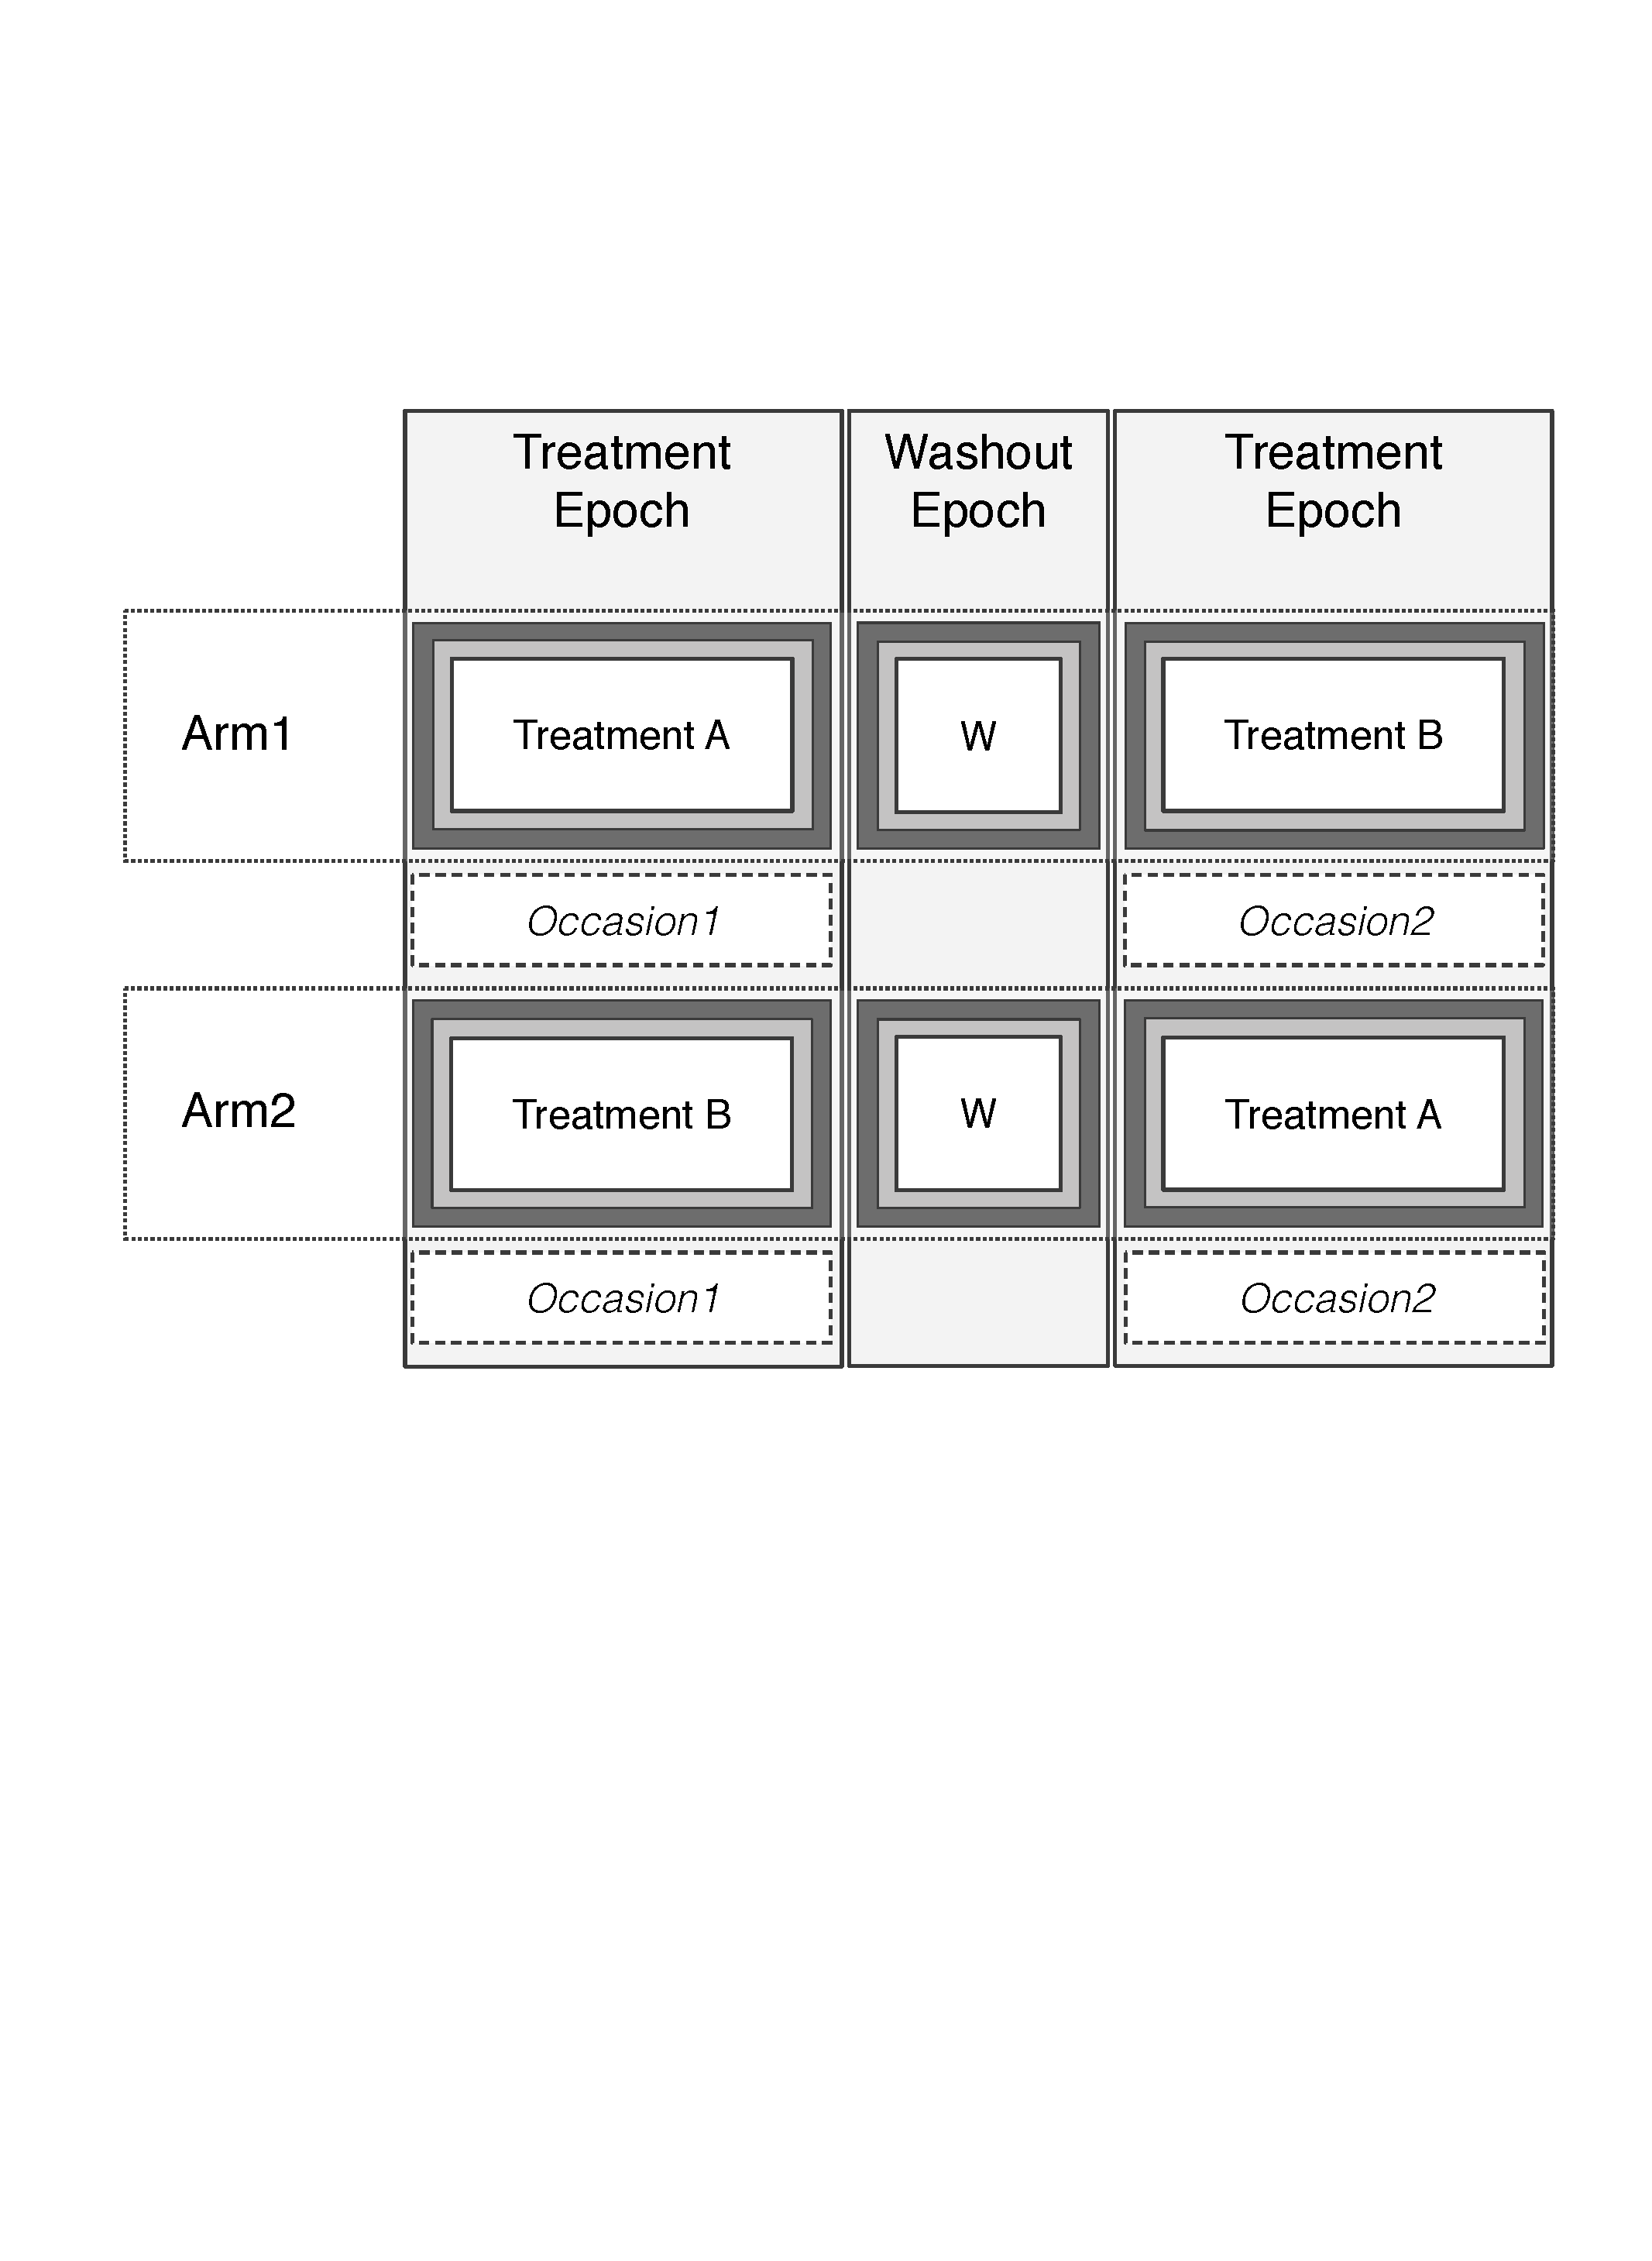
\includegraphics[width=0.7\linewidth]{pics/TwoArmsThreeEpochs_withWashout.pdf}
\caption{Schematic representation of a crossover design with washout. 
%The reader is referred to Figure \ref{fig:templateTrialDesign} for the colour code used to identify the elements of a trial. 
See tables \ref{fig:eg4:segmentCellArmEpoch} 
and \ref{fig:eg4:epochDef} for the detailed definition of segments, cells, arms, epochs
and occasions in this example.}
\label{fig:TwoArmsThreeEpochs_withWashout}
\end{figure}

%\noindent
\begin{table}[h]
\begin{center}
\begin{tabular}{lrr}\toprule
Arm & \textbf{1} & \textbf{2} \\\midrule
Number of subjects & 33 & 33\\
Dose variable & \var{D} & \var{D} \\
Dosing Amount & 100 & 150 \\
Dose Units & $\mg$ & $\mg$  \\
Dose per kg & no & no \\
Dosing times (h) &  0 &  0 \\
\bottomrule
\end{tabular}
\end{center}
\caption{Arms overview with dosing specification.}
\label{tab:ArmOverview}
\end{table}


%%%%%%%%%%%%%%%%%%%%%%%%%%%%%%%%%%%%%%%%%%%%%%%%%%%%%%%%%%%%%%%%
\subsubsection{Trial Design}
The model features a basic crossover design (see Figure
\ref{fig:TwoArmsThreeEpochs_withWashout}) with washout period and inter-occasion
variability (IOV). There are two treatments and the subjects are
organised into two arms that start with a different treatment. In
between each treatment there is a washout period during which time the
drug is eliminated from each subject. 
In the model the occasions, provide a second level of variability -- 
IOV \index{variability!IOV} (see section \ref{sec:variabilityModel}).  
This is summarised in Figure \ref{fig:eg4-IOV_2levels} (see also the listing 
in section \ref{eg4:variabilityModel}, showing relevant code 
within the element \xelem{VariabilityModel}).

The model also uses covariates to model the variability within the
model and so the treatments, the sequence of treatments (i.e.\xspace treatments A, B or
B,A) and the occasion itself are described in the covariate section
below.

\begin{figure}[ht!]
\centering
 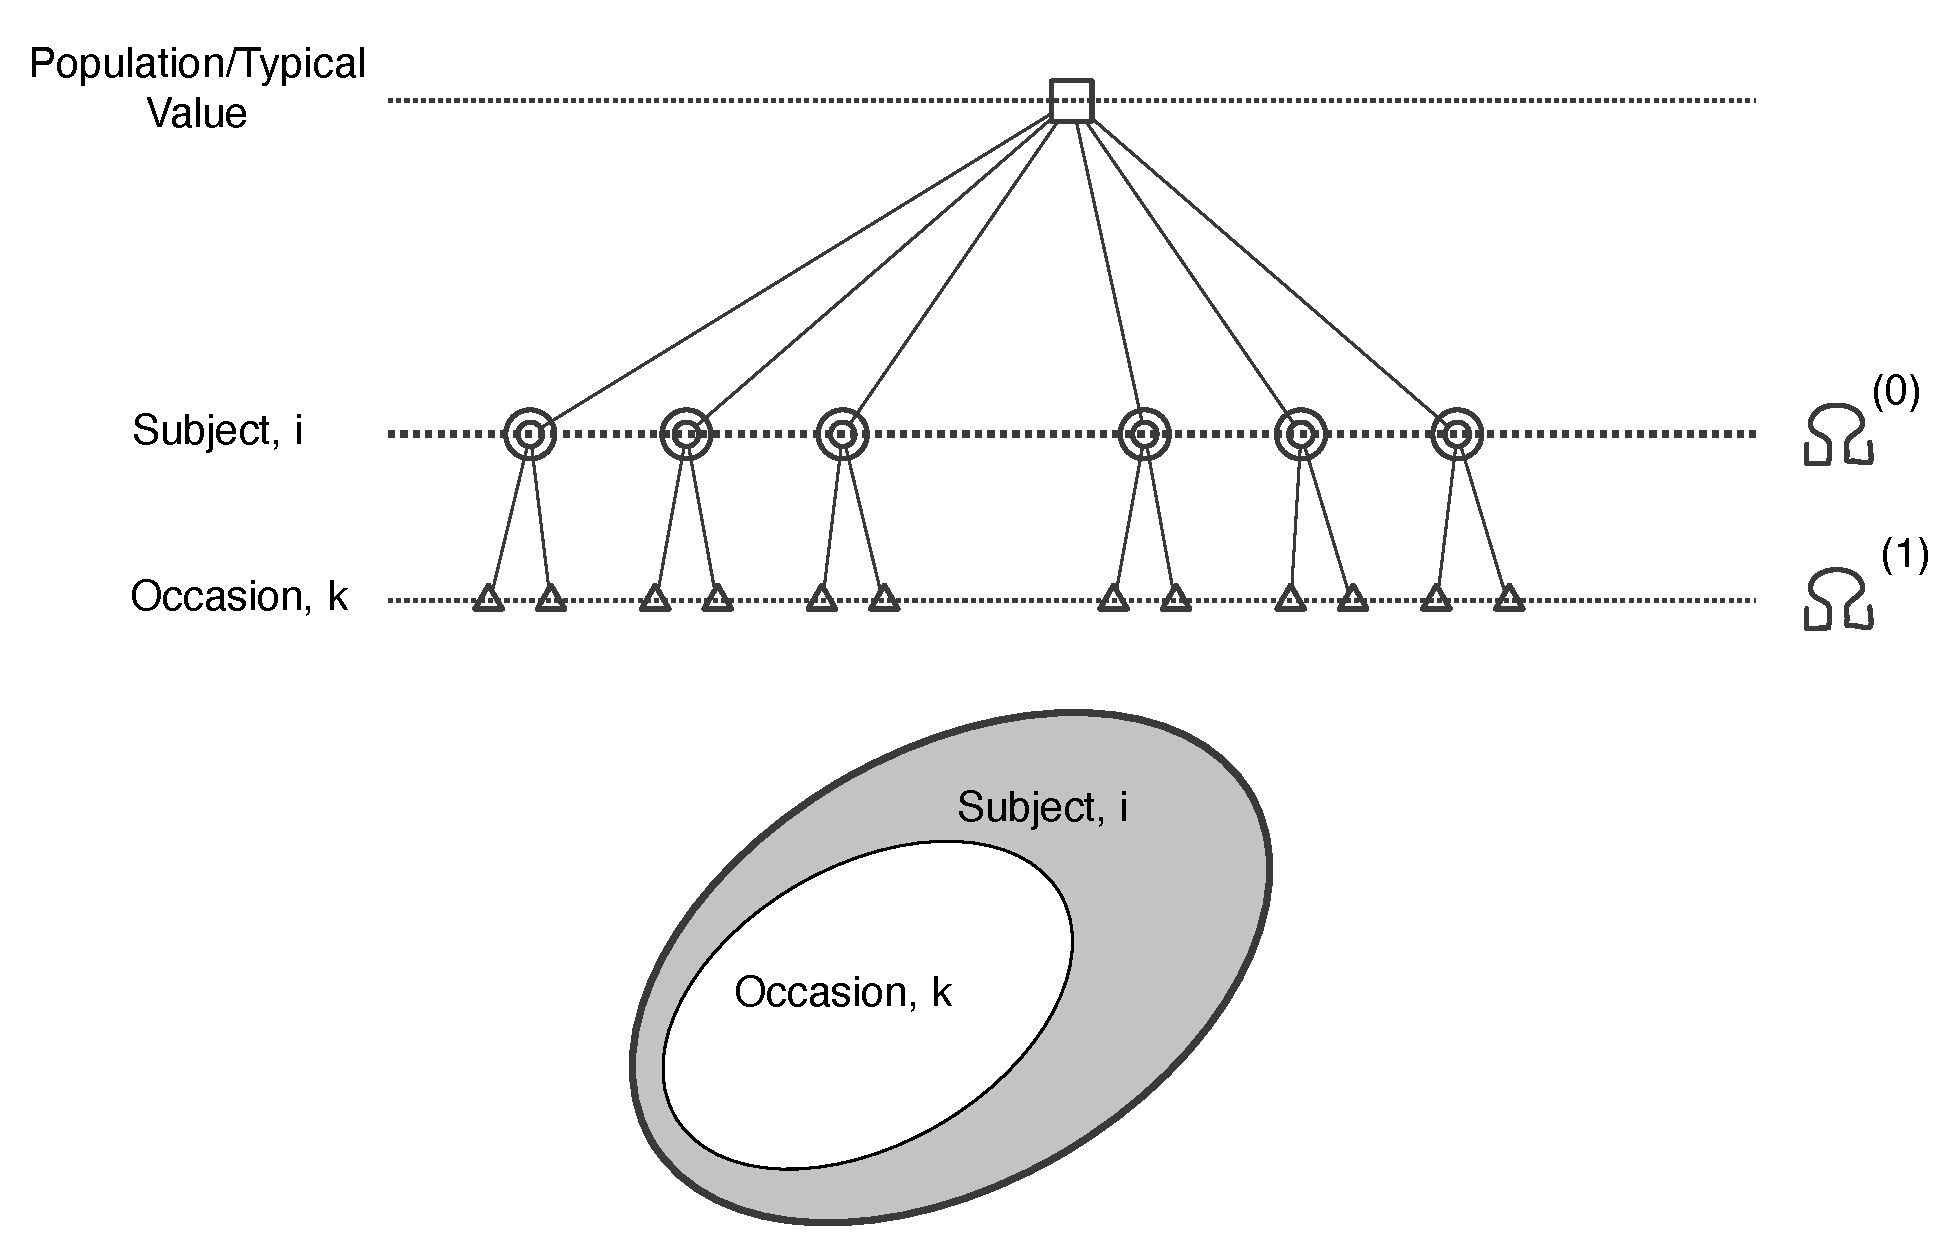
\includegraphics[width=120mm]{pics/IOV_2levels}
\caption{Two levels of variability -- inter-individual and inter-occasion within individual variability.}
\label{fig:eg4-IOV_2levels}
\end{figure}


%%%%%%%%%%%%%%%%%%%%%%%%%%%%%%%%%%%%%%%%%%%%%%%%%%%%%%%%%%%%%%%%
\subsubsection{Covariate Model}
\label{eg4:covariates-defn}

As discussed about all covariates are used to capture the explained variability in the model, 
see Table \ref{tab:CovariatesOverview}, and the \emph{Occasion} additionally
the unexplained expressed as the $\eta^{(+1)}$ random effects associated with CL and V.

\begin{table}[h]
\begin{center}
\begin{tabular}{lrrrr}\toprule
 & \textbf{Sex} &{\color{red}\textbf{Treat}}&{\color{mediumgreen}\textbf{TreatSeq}}&{\color{magenta}\textbf{Occasion}}\\\midrule
Type & Categorical & Categorical & Categorical & Categorical  \\
Category Count & 2 & 2 & 2 & 2\\
Categories & F, M & A, B & AB,BA & 1, 2\\
Reference & F & A & AB & 1\\
%Reference Probability & $14/36$ & 0.5  & 0.5  & 0.5\\
\bottomrule
\end{tabular}
\end{center}
\caption{Covariates overview.}
\label{tab:CovariatesOverview}
\end{table}

%%%%%%%%%%%%%%%%%%%%%%%%%%%%%%%%%%%%%%%%%%%%%%%%%%%%%%%%%%%%%%%%
\subsubsection{Parameter Model}

The parameter model includes random effects that represent the IIV and
{\color{lightblue}IOV} levels of variability. It also relates the
parameters to the covariates described above:
\begin{align}
\log(ka_{i}) &= \log(ka_{pop}) +
{\color{mediumgreen}\beta_{ka,TreatSeq}}1_{TreatSeq_i=AB} +
\eta_{ka,i} \label{eqn:eg4-param-ka}\\
\begin{split}
\log(V_{ik}) &= \log(V_{pop}) + {\boldsymbol \beta_V}1_{S_i=F} +
{\color{magenta}\beta_{V,OCC}} 1_{OCC_{ik}=1} \\
&\quad+ {\color{red}\beta_{V,Treat}}1_{Treat_{ik}=A} + {\color{mediumgreen}\beta_{V,TreatSeq}}1_{TreatSeq_i=AB} \\
		& \quad+ \eta_{V,i}^{(0)} +  {\color{lightblue} \eta_{V,ik}^{(+1)} }
\end{split} \label{eqn:eg4-parameter-v}\\
\begin{split}
\log(\CL_{ik}) &= \log(\CL_{pop}) + {\boldsymbol \beta_{\CL}}1_{S_i=F}
+ {\color{magenta}\beta_{\CL,OCC}} 1_{OCC_{ik}=1}\\
&\quad + \eta_{\CL,i}^{(0)} + {\color{lightblue} \eta_{Cl,ik}^{(+1)} }
\end{split}\nonumber
\end{align}
where
\begin{gather*}
\eta_{ka,i}^{(0)} \sim \mathcal{N}(0, \omega_{ka}), \quad \eta_{V,i}^{(0)} \sim \mathcal{N}(0, \omega_{V}), \quad \eta_{\CL,i}^{(0)} \sim \mathcal{N}(0, \omega_{\CL}),  \\
 {\color{lightblue} \eta_{V,ik}^{(+1)} \sim \mathcal{N}(0,\gamma_V)}, \quad
 {\color{lightblue} \eta_{\CL,ik}^{(+1)} \sim \mathcal{N}(0, \gamma_{\CL})}
\end{gather*}

The full variance-covariance matrices for our model read
\begin{gather}
 \Omega^{(0)} =
 \begin{pmatrix}
  \omega_{ka}^2 	& 0 				& 0  \\
   			  	& \omega_{V}^2	& 0 	\\
  				& 				& \omega_{\CL}^2\\
 \end{pmatrix}\label{eqn:eg4-covariance-mat}\\
 \Omega^{(+1)} =
 \begin{pmatrix}
0 & 0 & 0\\
 & \gamma_{V}^2	& 0 	\\
 & & \gamma_{\CL}^2\\
 \end{pmatrix}\label{eqn:eg4-gamma-mat}
\end{gather}


%%%%%%%%%%%%%%%%%%%%%%%%%%%%%%%%%%%%%%%%%%%%%%%%%%%%%%%%%%%%%%%%
\subsubsection{Structural model}

The model is first order absorption with linear elimination. This is the equivalent to 
oral1\_1cpt\_kaVCl (model 8) from \cite[Appendix I]{Bertrand:2008}.


%%%%%%%%%%%%%%%%%%%%%%%%%%%%%%%%%%%%%%%%%%%%%%%%%%%%%%%%%%%%%%%%
\subsubsection{Observation model}

We apply a residual error models to the output variable \var{C}.

%\noindent
\begin{center}
\begin{tabular*}{0.6\textwidth}{@{\extracolsep{\fill}} >{\bfseries}l l}\toprule
Output Variable  & \textbf{\itshape C} \\\midrule
Observations Name & Concentration\\
Units & $\mg/l$ \\
Observations Type & Continuous \\
Residual Error Model & Combined \\
Error Model Parameters & $a = 0.1,\quad b=0.1$\\
\bottomrule
\end{tabular*}
\end{center}


%%%%%%%%%%%%%%%%%%%%%%%%%%%%%%%%%%%%%%%%%%%%%%%%%%%%%%%%%%%%%%%%
\subsubsection{Modelling Steps}
Compared to the last example, we have define here two tasks:
\begin{itemize}
\item Estimation of population paramaters.
\item Estimation of the individual parameters.
\end{itemize}

%%%%%%%%%%%%%%%%%%%%%%%%%%%%%%%%%%%%%%%%%%%%%%%%%%%%%%%%%%%%%%%%
\subsection{Trial Design}

We have summaries the dosing regimen and organisation of the trial
design below, see also Figure \ref{fig:TwoArmsThreeEpochs_withWashout}.

\begin{table}[htdp!]
\begin{center}
\begin{tabular}{ccccccc}
\hline
Segment&Activity & Treatment & DoseTime & DoseSize & Target Variable \\
\hline
TA& OR1 &  OR bolus & $0:12:72$ & 150 & D \\
TA& OR2 &  OR bolus & $0:24:72$ & 100 & D \\
\hline
\end{tabular}
\end{center}
\caption{Segment/activity overview.}
\label{fig:eg4:segmentCellArmEpoch}
\end{table}

\begin{table}[htdp!]
\begin{center}
\begin{tabular}{cccc}
\hline
Epoch & Occasion & Start time & End time \\
\hline
Treatment Epoch & OCC1 & 0 &  180  \\
Washout & -- & 0 &  10  \\
Treatment Epoch & OCC2 & 0 &  180  \\
\hline
\end{tabular}
\end{center}
\caption{Epoch and occasion definition.}
\label{fig:eg4:epochDef}
\end{table}


%%%%%%%%%%%%%%%%%%%%%%%%%%%%%%%%%%%%%%%%%%%%%%%%%%%%%%%%%%%%%%%%
\subsubsection{Structure}
The implementation of the treatments, in \pharmml we use the
\xelem{Activity} element, is different compared to the previous example. 
See Table \ref{fig:eg4:segmentCellArmEpoch} for the details. The difference
is that now we have one dose administered at multiple dosing time points 
instead of single time point. See the following listing 
%\inputxml{exp6_dosingTimes.xml}
\lstset{language=XML}
\begin{lstlisting}
            <Activity oid="d1">
                <Bolus>
                    <DoseAmount inputTarget="parameter">
                        <ct:SymbRef blkIdRef="sm1" symbIdRef="D"/>
                        <ct:Assign>
                            <ct:Real>150</ct:Real>
                        </ct:Assign>
                    </DoseAmount>
                    <DosingTimes>
                        <ct:SymbRef blkIdRef="sm1" symbIdRef="tD"/>
                        <ct:Assign>
                            <ct:Sequence>
                                <ct:Begin><ct:Real>0</ct:Real></ct:Begin>
                                <ct:StepSize><ct:Real>12</ct:Real></ct:StepSize>
                                <ct:End><ct:Real>72</ct:Real></ct:End>
                            </ct:Sequence>
                        </ct:Assign>
                    </DosingTimes>
                </Bolus>
            </Activity>
\end{lstlisting}

how one can describe it within the \xelem{DosingTimes} element using the \xelem{Sequence}
structure defining the start/end times and step size.

Table \ref{fig:eg4:epochDef} gives an overview of the \var{Epochs} and \var{Occasions} 
in this example. Here, the occasions overlap with the epochs, the start and end times 
are identical, this is not always the case, the occasions can span one or more epochs. 
The \var{Washout} epoch is given here with start/end times as well which is in fact 
a redundant piece of information (but required by construction of an \var{Epoch})
as a \var{Washout} always assumes total reset of all drug amounts. 

As discussed in the section \ref{subsec:TrialStructure}, in \xelem{Structure} block 
we encode the variability which is located below the subject (see the 
hierarchy of the random variability discussed in section \ref{sec:variabilityModel}).
We call it the \textit{inter-occasion variability}, IOV. The following listing 
%\inputxml{exp6_structure_part3.xml} 
\lstset{language=XML}
\begin{lstlisting}
            <ObservationsEvent oid="occasions"> 
                <ArmRef oidRef="a1"/>
                <ArmRef oidRef="a2"/>
                <ct:VariabilityReference>
                    <ct:SymbRef blkIdRef="vm1" symbIdRef="iov1"/>
                </ct:VariabilityReference>
                <ObservationGroup oid="occ1">
                    <EpochRef oidRef="ep1"/>
                </ObservationGroup>
                <ObservationGroup oid="occ2">
                    <EpochRef oidRef="ep3"/>
                </ObservationGroup>
            </ObservationsEvent>
        </Structure>
\end{lstlisting}

shows how this is done. 
In this case the occasions coincide with the epochs 
so we use the \xelem{EpochRef} element. Alternatively, we could use the \xelem{Period}
element to define explicitly the start and end times of the occasions as shown 
in this listing: 
%\inputxml{exp6_structure_part4.xml}
\lstset{language=XML}
\begin{lstlisting}
            <!-- alternative -->
            <ObservationsEvent oid="occasions"> 
                <ArmRef oidRef="a1"/>
                <ArmRef oidRef="a2"/>
                <ct:VariabilityReference>
                    <ct:SymbRef blkIdRef="vm1" symbIdRef="iov1"/>
                </ct:VariabilityReference>
                <ObservationGroup oid="occ1">
                    <Period>
                        <Start><ct:Real>0</ct:Real></Start>
                        <End><ct:Real>180</ct:Real></End>
                    </Period>
                </ObservationGroup>
                <ObservationGroup oid="occ2">
                    <Period>
                        <Start><ct:Real>0</ct:Real></Start>
                        <End><ct:Real>180</ct:Real></End>
                    </Period>
                </ObservationGroup>
            </ObservationsEvent>
        </Structure>
\end{lstlisting}

This is of course very useful if the occasions do not
coincide with the epochs, or there are two or more occasions within one epoch.
In this case we set the \var{Start} and \var{End} times to $0$ and $180$, respectively.
These are exactly the same time points as are used in the epoch definition 
(see the first listing in section \ref{eg4_subsec:trialDesign} for how to encode epochs in the 
\xelem{Structure} definition).   


%%%%%%%%%%%%%%%%%%%%%%%%%%%%%%%%%%%%%%%%%%%%%%%%%%%%%%%%%%%%%%%%
\subsubsection{Population}
We pick up where we left off in the \xelem{Structure}, implementing
the hooks to the variability structure. The aspect we have not covered
yet is related to IIV.  The \xelem{Population} element is the place to
define any subject related variability and those levels above
it. The following listing shows how this works 
%\inputxml{exp6_population_part0.xml}
\lstset{language=XML}
\begin{lstlisting}
        <Population>
            <ct:VariabilityReference>
                <ct:SymbRef blkIdRef="vm1" symbIdRef="indiv"/>
            </ct:VariabilityReference>
            <!-- SKIP -->
\end{lstlisting}
In this example we deal only with the IIV and a level below it, so this is 
all we have to encode variability-wise at this point.

The next part of the \xelem{Population} block was discussed previously. 
Beside the standard assignment of subjects to an \var{Arm}
and providing information regarding \var{SEX}, we need to encode the information
about study design related covariates, see Table \ref{tab:CovariatesOverview}. 
Treatment type, \var{TREAT} which varies in this cross-over design as the study 
progress from \var{Epoch1} to \var{Epoch3}, is considered here as covariate.
And so are the treatment sequence, \var{TREATSEQ}, and occasions associated
with EPOCHs. 
This table is populated with data as can be seen in the following listing 
%\inputxml{exp6_population_part2.xml}
\lstset{language=XML}
\begin{lstlisting}
<ColumnMapping>
    <ds:ColumnRef columnIdRef="SEX"/>
    <ct:SymbRef blkIdRef="cm1" symbIdRef="Sex"/>
</ColumnMapping>
<ColumnMapping>
    <ds:ColumnRef columnIdRef="TREAT"/>
    <ct:SymbRef blkIdRef="cm1" symbIdRef="Treat"/>
</ColumnMapping>
<ColumnMapping>
    <ds:ColumnRef columnIdRef="TREATSEQ"/>
    <ct:SymbRef blkIdRef="cm1" symbIdRef="TreatSeq"/>
</ColumnMapping>
<ColumnMapping>
    <ds:ColumnRef columnIdRef="EPOCH"/>
    <ct:SymbRef symbIdRef="Occasion"/>
    <ds:CategoryMapping>
        <ds:Map dataSymbol="ep1" modelSymbol="occ1"/>
        <ds:Map dataSymbol="ep3" modelSymbol="occ2"/>
    </ds:CategoryMapping>
</ColumnMapping>
<ds:DataSet>
    <ds:Definition>
        <ds:Column columnId="ID" columnType="id" valueType="string" columnNum="1"/>
        <ds:Column columnId="ARM" columnType="arm" valueType="id" columnNum="2"/>
        <ds:Column columnId="SEX" columnType="covariate" valueType="string" columnNum="3"/>
        <ds:Column columnId="EPOCH" columnType="epoch" valueType="id" columnNum="4"/>
        <ds:Column columnId="TREAT" columnType="covariate" valueType="string" columnNum="5"/>
        <ds:Column columnId="TREATSEQ" columnType="covariate" valueType="string" columnNum="6"/>
    </ds:Definition>
    <ds:Table>
        <!-- arm1 -->
        <ds:Row><ct:String>1</ct:String><ct:Id>a1</ct:Id><ct:Id>M</ct:Id><ct:Id>ep1</ct:Id>
        											<ct:Id>A</ct:Id><ct:Id>AB</ct:Id></ds:Row>
        <ds:Row><ct:String>1</ct:String><ct:Id>a1</ct:Id><ct:Id>M</ct:Id><ct:Id>ep3</ct:Id>
        											<ct:Id>B</ct:Id><ct:Id>AB</ct:Id></ds:Row>
        <ds:Row><ct:String>2</ct:String><ct:Id>a1</ct:Id><ct:Id>M</ct:Id><ct:Id>ep1</ct:Id>
        											<ct:Id>A</ct:Id><ct:Id>AB</ct:Id></ds:Row>
        <ds:Row><ct:String>2</ct:String><ct:Id>a1</ct:Id><ct:Id>M</ct:Id><ct:Id>ep3</ct:Id>
        											<ct:Id>B</ct:Id><ct:Id>AB</ct:Id></ds:Row>
        <!-- arm2 -->
        <ds:Row><ct:String>9</ct:String><ct:Id>a2</ct:Id><ct:Id>M</ct:Id><ct:Id>ep1</ct:Id>
        											<ct:Id>B</ct:Id><ct:Id>BA</ct:Id></ds:Row>
        <ds:Row><ct:String>9</ct:String><ct:Id>a2</ct:Id><ct:Id>M</ct:Id><ct:Id>ep3</ct:Id>
        											<ct:Id>A</ct:Id><ct:Id>BA</ct:Id></ds:Row>
        <ds:Row><ct:String>10</ct:String><ct:Id>a2</ct:Id><ct:Id>M</ct:Id><ct:Id>ep1</ct:Id>
        											<ct:Id>B</ct:Id><ct:Id>BA</ct:Id></ds:Row>
        <ds:Row><ct:String>10</ct:String><ct:Id>a2</ct:Id><ct:Id>M</ct:Id><ct:Id>ep3</ct:Id>
        											<ct:Id>A</ct:Id><ct:Id>BA</ct:Id></ds:Row>
    </ds:Table>
</ds:DataSet>
</Population>
\end{lstlisting}
shows few subject data records for \var{Arm1} and \var{Arm2}. We have used 
in this example a new element, \xelem{CategoryMapping}, which use will be 
discussed in detail later in Section \ref{sec:eg4-NONMEMdataset}.


%%%%%%%%%%%%%%%%%%%%%%%%%%%%%%%%%%%%%%%%%%%%%%%%%%%%%%%%%%%%%%%%
\subsection{Variability Model}
\label{eg4:variabilityModel}

In this example the variability model is more complex than before, with IIV\index{variability!IIV} 
and IOV\index{variability!IOV} levels of variability, see Figure \ref{fig:eg4-IOV_2levels}. 
At this point in the \pharmml document we need to define the variability levels to be 
used in the rest of the document. You can see in the following listing 
%\inputxml{exp6_iov.xml}
\lstset{language=XML}
\begin{lstlisting}
        <VariabilityModel blkId="vm1" type="parameterVariability">
            <Level referenceLevel="true" symbId="indiv"/>
            <Level symbId="iov1">
                <ParentLevel>
                    <ct:SymbRef symbIdRef="indiv"/>
                </ParentLevel>
            </Level>
        </VariabilityModel>
\end{lstlisting}

that this is done by listing the variability levels using the \xelem{VariabilityLevel} 
element and their relationship. There are few important points to note here:
\begin{enumerate}
\item 
If more then one variability levels is used/defined in a model, it is useful to specify 
the reference level explicitly using the attribute \xatt{referenceLevel="true"} as can be seen
for the level called \xatt{indiv}. As explained previously it is not strictly required when
the dataset and column mapping are exhaustively defined but it simplifies the 
understudying of the variability model structure.
\item There is parent-child relationship between the levels of variability. The reference 
\var{Subject} level is referenced with the attribute \xatt{symbId="indiv"} is above the 
\var{Occasion} level, referenced with the attribute \xatt{symbId="iov1"} which is  
what is done using the \xelem{ParentLevel} in the listing.
\item The name given to a level, using the \xatt{symbId} attribute, is \textbf{not} 
significant. We used the names \var{iov1} and \var{indiv} to provide clarity in other 
parts of the example document.
\item The type of each variability level (e.g.,\xspace between-subject, inter-occasion, 
between-centre) is not defined here or in the Model Definition as a 
whole\footnote{N.B.,\xspace The numerical levels described in the variability 
model (section \ref{sec:variabilityModel}) are not used.}.
\end{enumerate}

In this example the \pharmml document tells us that there are two variability levels,
the reference \xatt{indiv} level and the lower level of variability is 
called ``\texttt{iov1}''\index{variability!IOV}\@. Moreover, we need to know their order 
relative to each other.


%%%%%%%%%%%%%%%%%%%%%%%%%%%%%%%%%%%%%%%%%%%%%%%%%%%%%%%%%%%%%%%%
\subsection{Covariate Model}

The covariate model describes categorical covariates, listed in Table 
\ref{tab:CovariatesOverview}, \index{covariate!categorical}which we have 
not seen in the previous examples. 

Because this is an estimation example no probabilities are provided and only the 
categories are defined, placed in the \xelem{Categorical} element. 
Then the implementation of each covariate follows the same
schema, which will be explained for the gender covariate \var{Sex}. 
There are obviously two categories the covariate can be associate with \textit{F} or \textit{M},
which are encoded using the \xelem{Category} element followed by an optional
\xelem{Name}. 

See the following listing how this is done 
%\inputxml{exp6_covariates.xml}
\lstset{language=XML}
\begin{lstlisting}
        <CovariateModel blkId="cm1">
            <Covariate symbId="Sex">
                <Categorical>
                    <Category catId="F">
                        <ct:Name>Female</ct:Name>
                    </Category>
                    <Category catId="M">
                        <ct:Name>Male</ct:Name>
                    </Category>
                </Categorical>
            </Covariate>
            <Covariate symbId="Treat">
                <Categorical>
                    <Category catId="A"/>
                    <Category catId="B"/>
                </Categorical>
            </Covariate>
            <Covariate symbId="TreatSeq">
                <Categorical>
                    <Category catId="AB">
                        <ct:Name>AB</ct:Name>
                    </Category>
                    <Category catId="BA">
                        <ct:Name>BA</ct:Name>
                    </Category>
                </Categorical>
            </Covariate>
            <Covariate symbId="Occasion">
                <Categorical>
                    <Category catId="occ1">
                        <ct:Name>1</ct:Name>
                    </Category>
                    <Category catId="occ2">
                        <ct:Name>2</ct:Name>
                    </Category>
                </Categorical>
            </Covariate>
        </CovariateModel>
\end{lstlisting}


%%%%%%%%%%%%%%%%%%%%%%%%%%%%%%%%%%%%%%%%%%%%%%%%%%%%%%%%%%%%%%%%
\subsection{Parameter Model}

In example \egref{1} (section \ref{sec:eg1}) we showed you how to define an individual
parameter in \pharmml and relate that to a continuous covariate. Now
in this example we will show how \pharmml can be used to describe
parameters that have multiple levels of variability and are related to
categorical covariates\index{covariate!categorical}.


In the following listing 
%\inputxml{exp6_ka.xml}
\lstset{language=XML}
\begin{lstlisting}
            <SimpleParameter symbId="omega_ka"/>
            <SimpleParameter symbId="pop_ka"/>
            <RandomVariable symbId="eta_ka">
                <ct:VariabilityReference>
                    <ct:SymbRef blkIdRef="vm1" symbIdRef="indiv"/>
                </ct:VariabilityReference>
                <NormalDistribution xmlns="http://www.uncertml.org/3.0" definition="">
                    <mean><rVal>0</rVal></mean>
                    <stddev><var varId="omega_ka"/></stddev>
                </NormalDistribution>
            </RandomVariable>
            <IndividualParameter symbId="ka">
                <GaussianModel>
                    <Transformation>log</Transformation>
                    <LinearCovariate>
                        <PopulationParameter>
                            <ct:Assign><ct:SymbRef symbIdRef="pop_ka"/></ct:Assign>
                        </PopulationParameter>
                        <Covariate>
                            <ct:SymbRef blkIdRef="cm1" symbIdRef="TreatSeq"/>
                            <FixedEffect>
                                <ct:SymbRef symbIdRef="beta_ka_treatseq"/>
                                <Category catId="AB"/>
                            </FixedEffect>
                        </Covariate>
                    </LinearCovariate>
                    <RandomEffects>
                        <ct:SymbRef symbIdRef="eta_ka"/>
                    </RandomEffects>
                </GaussianModel>
            </IndividualParameter>
\end{lstlisting}

 we show the definition of
parameter \var{ka}, which corresponds to (\ref{eqn:eg4-param-ka}). You
should be familiar with this structure by now, but you should take
note of the \xelem{Category} element within the \xelem{FixedEffect}
element. We use this to tell \pharmml that this fixed effect is related
to the ``\texttt{AB}'' category of the \var{TreatSeq} covariate. This
is equivalent to the expression
$\beta_{ka,TreatSeq}1_{TreatSeq_i=AB}$ in
(\ref{eqn:eg4-param-ka}). Note that it is possible to do this more
than once, for example if the covariate has more than two categories.


Parameter \var{ka} has only one level of variability, but this 
%\inputxml{exp6_V_part1.xml} 
\lstset{language=XML}
\begin{lstlisting}
            <SimpleParameter symbId="pop_V"/>
            <SimpleParameter symbId="omega_V"/>
            <SimpleParameter symbId="gamma_V"/>
            <SimpleParameter symbId="beta_V"/>
            <SimpleParameter symbId="beta_V_occ1"/>
            <SimpleParameter symbId="beta_V_Treat"/>
            <SimpleParameter symbId="beta_V_TreatSeq"/>
            <RandomVariable symbId="eta_V">
                <ct:VariabilityReference>
                    <ct:SymbRef blkIdRef="vm1" symbIdRef="indiv"/>
                </ct:VariabilityReference>
                <NormalDistribution xmlns="http://www.uncertml.org/3.0" definition="">
                    <mean><rVal>0</rVal></mean>
                    <stddev><var varId="omega_V"/></stddev>
                </NormalDistribution>
            </RandomVariable>
            <RandomVariable symbId="kappa_V">
                <ct:VariabilityReference>
                    <ct:SymbRef blkIdRef="vm1" symbIdRef="iov1"/>
                </ct:VariabilityReference>
                <NormalDistribution xmlns="http://www.uncertml.org/3.0" definition="">
                    <mean><rVal>0</rVal></mean>
                    <stddev><var varId="gamma_V"/></stddev>
                </NormalDistribution>
            </RandomVariable>
\end{lstlisting}

and this listing 
%\inputxml{exp6_V_part2.xml}
\lstset{language=XML}
\begin{lstlisting}
            <IndividualParameter symbId="V">
                <GaussianModel>
                    <Transformation>log</Transformation>
                    <LinearCovariate>
                        <PopulationParameter>
                            <ct:Assign><ct:SymbRef symbIdRef="pop_V"/></ct:Assign>
                        </PopulationParameter>
                        <Covariate>
                            <ct:SymbRef blkIdRef="cm1" symbIdRef="sex"/>
                            <FixedEffect>
                                <ct:SymbRef symbIdRef="beta_V"/>
                                <Category catId="F"/>
                            </FixedEffect>
                        </Covariate>
                        <Covariate>
                            <ct:SymbRef blkIdRef="cm1" symbIdRef="Occasion"/>
                            <FixedEffect>
                                <ct:SymbRef symbIdRef="beta_V_occ1"/>
                                <Category catId="occ1"/>
                            </FixedEffect>
                        </Covariate>
                        <Covariate>
                            <ct:SymbRef blkIdRef="cm1" symbIdRef="Treat"/>
                            <FixedEffect>
                                <ct:SymbRef symbIdRef="beta_V_Treat"/>
                                <Category catId="A"/>
                            </FixedEffect>
                        </Covariate>
                        <Covariate>
                            <ct:SymbRef blkIdRef="cm1" symbIdRef="TreatSeq"/>
                            <FixedEffect>
                                <ct:SymbRef symbIdRef="beta_V_TreatSeq"/>
                                <Category catId="AB"/>
                            </FixedEffect>
                        </Covariate>
                    </LinearCovariate>
                    <RandomEffects>
                        <ct:SymbRef symbIdRef="eta_V"/>
                    </RandomEffects>
                    <RandomEffects>
                        <ct:SymbRef symbIdRef="kappa_V"/>
                    </RandomEffects>
                </GaussianModel>
            </IndividualParameter>
\end{lstlisting}

show how we describe parameter
\var{V} with both IIV and IOV levels of variability. Very simply we
add a \xelem{RandomVariable} for each level of variability and use
the \xatt{symbIdRef} attribute in the \xelem{RandomEffects} element 
to map the random effect to the appropriate variability model as defined at 
the beginning of the \xelem{ModelDefinition} element. 
Thus \var{eta\_V} and \var{kappa\_V} correspond to the 
random effects $\eta^{(0)}_{V,i}$ and $\eta^{(+1)}_{V,ik}$ in
(\ref{eqn:eg4-parameter-v}). This parameter is related to all four
covariates, but we only show the \var{Sex} covariate. The others
defined in a very similar manner as all the covariates in this model
contain just 2 categories.

%%% TODO
We will not show parameter \var{Cl} as it does not illustrate any new
concepts, nor are any of the random effects in the model
correlated. This does not mean there is no covariance matrix defined
within the \pharmml document. There is. The matrices in
(\ref{eqn:eg4-covariance-mat}) and (\ref{eqn:eg4-gamma-mat}) are
implicitly defined because the standard deviations of the random effects 
are explicitly defined and no correlation between them is defined.


%%%%%%%%%%%%%%%%%%%%%%%%%%%%%%%%%%%%%%%%%%%%%%%%%%%%%%%%%%%%%%%%
\subsection{NONMEM dataset}
\label{sec:eg4-NONMEMdataset}
Now we will describe the case when the data and trial design are sourced from the 
NONMEM dataset. Table \ref{tab:example4_dataSet} show a typical dataset required for 
an estimation task.
\begin{table}[htdp]
\begin{center}
\small
\begin{tabular}{lllccccccc}\toprule
ID	& TIME	& DV			& AMT	& OCC	& TREAT	& TREATSEQ	& SEX 	& MDV 	& EVID \\ \midrule
1	& 0		& .			& 100	& 1		& 1		& 12			& 0 		& 1		& 1 \\ 
1	& 0.25	& 2.1243964	& .		& 1		& 1		& 12			& 0 		& 0		& 0 \\ 
1	& 0.5	& 4.308573	& .		& 1		& 1		& 12			& 0 		& 0		& 0  \\ 
1	& 1		& 7.6059305	& .		& 1		& 1		& 12			& 0 		& 0		& 0  \\ 
1	& 2		& 6.9678311	& .		& 1		& 1		& 12			& 0 		& 0		& 0  \\ 
1	& 3.5	& 7.7741686	& .		& 1		& 1		& 12			& 0 		& 0		& 0  \\ 
...	& ...		& ...			& ...		& ...		&...		& ...			& ... 		& ...		& ...  \\
1	& 24		& 1.5194051	& .		& 1		& 1		& 12			& 0 		& 0		& 0  \\ 
1	& 0		& .			& 100	& 2		& 2		& 12			& 0 		& 0		& 0  \\ 
1	& 0.25	& 4.2049182	& .		& 2		& 2		& 12			& 0 		& 0		& 0  \\ 
1	& 0.5	& 7.2508737	& .		& 2		& 2		& 12			& 0 		& 0		& 0  \\ 
1	& 1		& 8.5792413	& .		& 2		& 2		& 12			& 0 		& 0		& 0  \\ 
1	& 2		& 8.5689542	& .		& 2		& 2		& 12			& 0 		& 0		& 0  \\ 
1	& 3.5	& 10.1764867	& .		& 2		& 2		& 12			& 0 		& 0		& 0  \\ 
...	& ...		& ...			& ...		& ...		&...		& ...			& ... 		& ...		& ...  \\
1	& 24		& 0.8831267	& .		& 2		& 2		& 12			& 0 		& 0		& 0  \\ 
2	& 0		& .			& 100	& 1		& 2		& 21			& 1 		& 0		& 0  \\ 
2	& 0.25	& 2.6643053	& .		& 1		& 2		& 21			& 1 		& 0		& 0  \\ 
...	& ...		& ...			& ...		& ...		&...		& ...			& ... 		& 0		& 0  \\ \bottomrule
\end{tabular}
\end{center}
\caption{A dataset used in example \theexamples.}
\label{tab:example4_dataSet}
\end{table}%
and the following code shows how the according dataset definition and column mappings 
\lstset{language=XML}
\begin{lstlisting}
        <ExternalDataSet toolName="NONMEM" oid="NMoid">
            <ColumnMapping>
                <ds:ColumnRef columnIdRef="ID"/>
                <ct:SymbRef blkIdRef="vm1" symbIdRef="indiv"/>
            </ColumnMapping>
            <ColumnMapping>
                <ds:ColumnRef columnIdRef="Time"/>
                <ct:SymbRef symbIdRef="t"/>
            </ColumnMapping>
            <ColumnMapping>
                <ds:ColumnRef columnIdRef="Y"/>
                <ct:SymbRef blkIdRef="om1" symbIdRef="Cc_obs"/>
            </ColumnMapping>
            <ColumnMapping>
                <ds:ColumnRef columnIdRef="AMT"/>
                <ct:SymbRef blkIdRef="sm1" symbIdRef="D"/>
            </ColumnMapping>
            <!-- mapping occasions column to the covariate model -->
            <ColumnMapping>
                <ds:ColumnRef columnIdRef="OCC"/>
                <ct:SymbRef blkIdRef="cm1" symbIdRef="Occasion"/>
                <ds:CategoryMapping>
                    <ds:Map modelSymbol="occ1" dataSymbol="1"/>
                    <ds:Map modelSymbol="occ2" dataSymbol="2"/>
                </ds:CategoryMapping>
            </ColumnMapping>
            <!-- mapping occasions column to the variability model -->
            <ColumnMapping>
                <ds:ColumnRef columnIdRef="OCC"/>
                <ct:SymbRef blkIdRef="vm1" symbIdRef="iov1"/>
            </ColumnMapping>
            <ColumnMapping>
                <ds:ColumnRef columnIdRef="TREAT"/>
                <ct:SymbRef blkIdRef="cm1" symbIdRef="Treat"/>
                <ds:CategoryMapping>
                    <ds:Map dataSymbol="1" modelSymbol="A"/>
                    <ds:Map dataSymbol="2" modelSymbol="B"/>
                </ds:CategoryMapping>
            </ColumnMapping>
            <ColumnMapping>
                <ds:ColumnRef columnIdRef="TREATSEQ"/>
                <ct:SymbRef blkIdRef="cm1" symbIdRef="TreatSeq"/>
                <ds:CategoryMapping>
                    <ds:Map dataSymbol="12" modelSymbol="AB"/>
                    <ds:Map dataSymbol="21" modelSymbol="BA"/>
                </ds:CategoryMapping>
            </ColumnMapping>
            <ColumnMapping>
                <ds:ColumnRef columnIdRef="SEX"/>
                <ct:SymbRef blkIdRef="cm1" symbIdRef="Sex"/>
                <ds:CategoryMapping>
                    <ds:Map dataSymbol="0" modelSymbol="M"/>
                    <ds:Map dataSymbol="1" modelSymbol="F"/>
                </ds:CategoryMapping>
            </ColumnMapping>
            
            <!-- map 'tD' and 'TIME' if 'AMT' != 0 -->
            <ColumnMapping>
                <ds:ColumnRef columnIdRef="TIME"/>
                <ds:Piecewise>
                    <math:Piece>
                        <ct:SymbRef blkIdRef="sm1" symbIdRef="tD"/>
                        <math:Condition>
                            <math:LogicBinop op="neq">
                                <ds:ColumnRef columnIdRef="AMT"/>
                                <ct:Real>0</ct:Real>
                            </math:LogicBinop>
                        </math:Condition>
                    </math:Piece>
                </ds:Piecewise>
            </ColumnMapping>

            <ds:DataSet>
                <ds:Definition>
                    <ds:Column columnId="ID" columnType="id" valueType="string" columnNum="1"/>
                    <ds:Column columnId="TIME" columnType="time" valueType="real" columnNum="2"/>
                    <ds:Column columnId="Y" columnType="dv" valueType="real" columnNum="3"/>
                    <ds:Column columnId="AMT" columnType="dose" valueType="real" columnNum="4"/>
                    <ds:Column columnId="OCC" columnType="covariate" valueType="int" columnNum="5"/>
                    <ds:Column columnId="TREAT" columnType="covariate" valueType="int" columnNum="6"/>
                    <ds:Column columnId="TREATSEQ" columnType="covariate" valueType="int" columnNum="7"/>
                    <ds:Column columnId="SEX" columnType="covariate" valueType="int" columnNum="8"/>
                </ds:Definition>
                <ds:ImportData oid="dataOid">
                    <ds:path>example4.csv</ds:path>
                    <ds:format>CSV</ds:format>
                    <ds:delimiter>COMMA</ds:delimiter>
                </ds:ImportData>
            </ds:DataSet>
        </ExternalDataSet>
\end{lstlisting}
The mapping of the column \emph{OCC} deserves a short description. It is mapped twice
\begin{itemize}
\item
first, to map the occasions to the according covariate in \xelem{CovariateModel} \emph{cm1}
\item
second, to map them to the variability level, \xatt{iov1}, associated with the occasions defined
in the \xelem{VariabilityModel} \emph{vm1}
\end{itemize}
Compared to the previous examples the column mappings contain a new 
element, the \xelem{CategoryMapping} and within the \xelem{Map} elements 
use when mapping categorical covariates and discrete data model categories. 
Its attributes \xatt{dataSymbol} and \xatt{modelSymbol} identify the according 
symbols used in the model definition and the dataset, respectively.
 
Consider for example the covariate \emph{TREATSEQ}, in the model it is 
much more intuitive to use the \emph{AB} or \emph{BA} symbol id's then 
the corresponding 12 or 21 identifiers required as the NONMEM datasets 
are not allowing strings. The latter is also the reason why in this case we much
more often use the \xelem{ds:CategoryMapping} element as the dataset and model
use different symbols for the identical categories.

\subsection{Covered in previous examples}
The remaining elements of this example to be encoded in \pharmml
are nearly identical to those described before, such as \xelem{EstimationStep}
and \xelem{StepDepend\-encies} within the \xelem{ModellingSteps} block,
and will not be discussed here.

%%%%%%%%%%%%%%%%%%%%%%%%%%%%%%%%%%%%%%%%%%%%%%%%%%%%%%%%%%%%%%%%
%%%%%%%%%%%%%%%%%%%%%%%%%%%%%%%%%%%%%%%%%%%%%%%%%%%%%%%%%%%%%%%%
%%%%%%%%%%%%%%%%%%%%%%%%%%%%%%%%%%%%%%%%%%%%%%%%%%%%%%%%%%%%%%%%
\eglabel{5}
\section{Example \theexamples: Estimation with individual dosing}
\label{sec:Ribba}

%%%%%%%%%%%%%%%%%%%%%%%%%%%%%%%%%%%%%%%%%%%%%%%%%%%%%%%%%%%%%%%%
\subsection{Description}
This example is based on \cite{Ribba:2012uq} and deals with a mathematical
model describing the inhibition of the tumour growth of low-grade glioma treated
with chemotherapy\footnote{The example is encoded in two versions,  
\xatt{example5.xml} and \xatt{example5\_NONMEM.xml}, with explicit encoded trial 
design and design sourced from a NONMEM datafile, respectively.}. 
Although previous estimation examples were complex
enough to illustrate most important aspects of the current \pharmml specification 
we would like briefly to discuss this example due to its role as a use case. It also 
illustrates a new feature of the language, the fact that we can encode explicitly 
using patient specific administration scenarios within the \xelem{TrialDesign} section.


%%%%%%%%%%%%%%%%%%%%%%%%%%%%%%%%%%%%%%%%%%%%%%%%%%%%%%%%%%%%%%%%
\subsection{Trial design}
We will start with the definition of \xelem{Structure}, \xelem{Population}. The next language element, 
\xelem{IndividualDosing}, is, as mentioned above.

%%%%%%%%%%%%%%%%%%%%%%%%%%%%%%%%%%%%%%%%%%%%%%%%%%%%%%%%%%%%%%%%
\subsubsection{Structure}
Figure \ref{fig:1Arm1Epoch_RibbaDesign} shows the design structure of this example 
consisting of one arm and one epoch, meaning there is one treatment type 'IV' for all patients. 
As explained in section \ref{sec:CTS} the design element \xelem{Cell} comprises the 
essential elements specifying the information about the arm, epoch and segment/activities. 
\xelem{Segment} contains treatment definition, here an IV bolus administration, 
defined in the \xelem{Activity} element. Figure \ref{fig:cellHierarchy_Ribba} shows 
the general relationship of these elements (left) and how it applies to the current example (right).
See the following listing 
%\inputxml{Ribba_structure.xml}
\lstset{language=XML}
\begin{lstlisting}
        <Structure>
            <Epoch oid="epoch1">
                <Start><ct:Real>0</ct:Real></Start>
                <End><ct:Real>200</ct:Real></End>
                <Order>1</Order>
            </Epoch>
            <Arm oid="arm1"/>
            <Cell oid="cell1">
                <EpochRef oidRef="epoch1"/>
                <ArmRef oidRef="arm1"/>
                <SegmentRef oidRef="TA"/>
            </Cell>
            <Segment oid="TA">
                <ActivityRef oidRef="bolusIV"/>
            </Segment>
            <Activity oid="bolusIV">
                <Bolus>
                    <DoseAmount inputTarget="derivativeVariable">
                        <ct:SymbRef blkIdRef="sm1" symbIdRef="C"/>
                    </DoseAmount>
                </Bolus>
            </Activity>
        </Structure> 
\end{lstlisting}
for the PharmML implementation.

\begin{figure}[ht!]
\centering
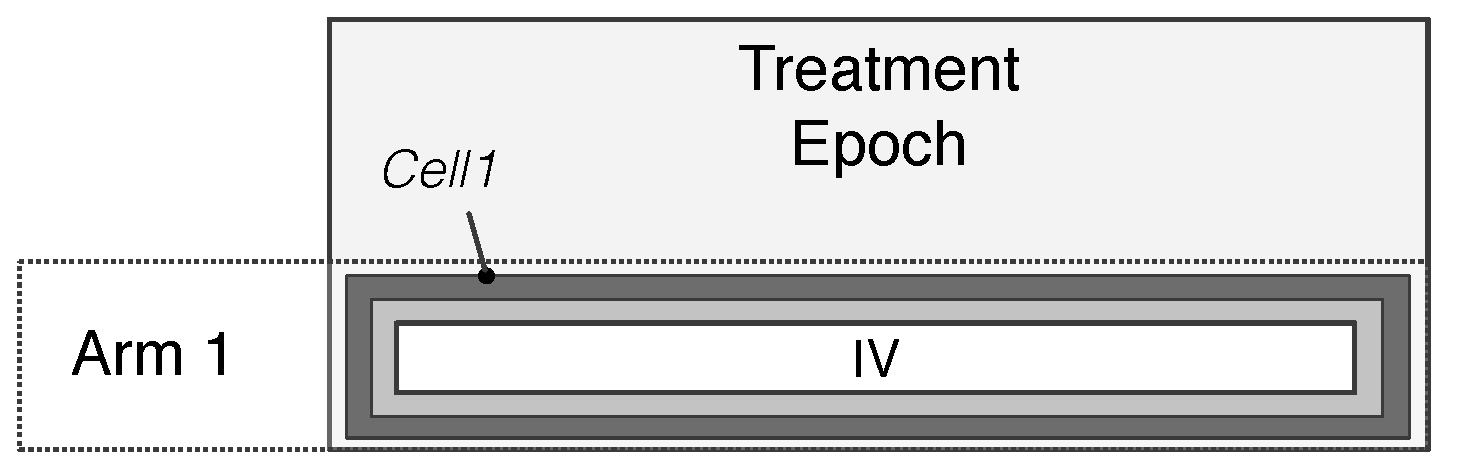
\includegraphics[width=0.7\linewidth]{pics/OneArmOneEpoch_IV}
\caption{Design overview: single arm design.}
\label{fig:1Arm1Epoch_RibbaDesign}
\end{figure}

\begin{figure}[ht!]
\centering
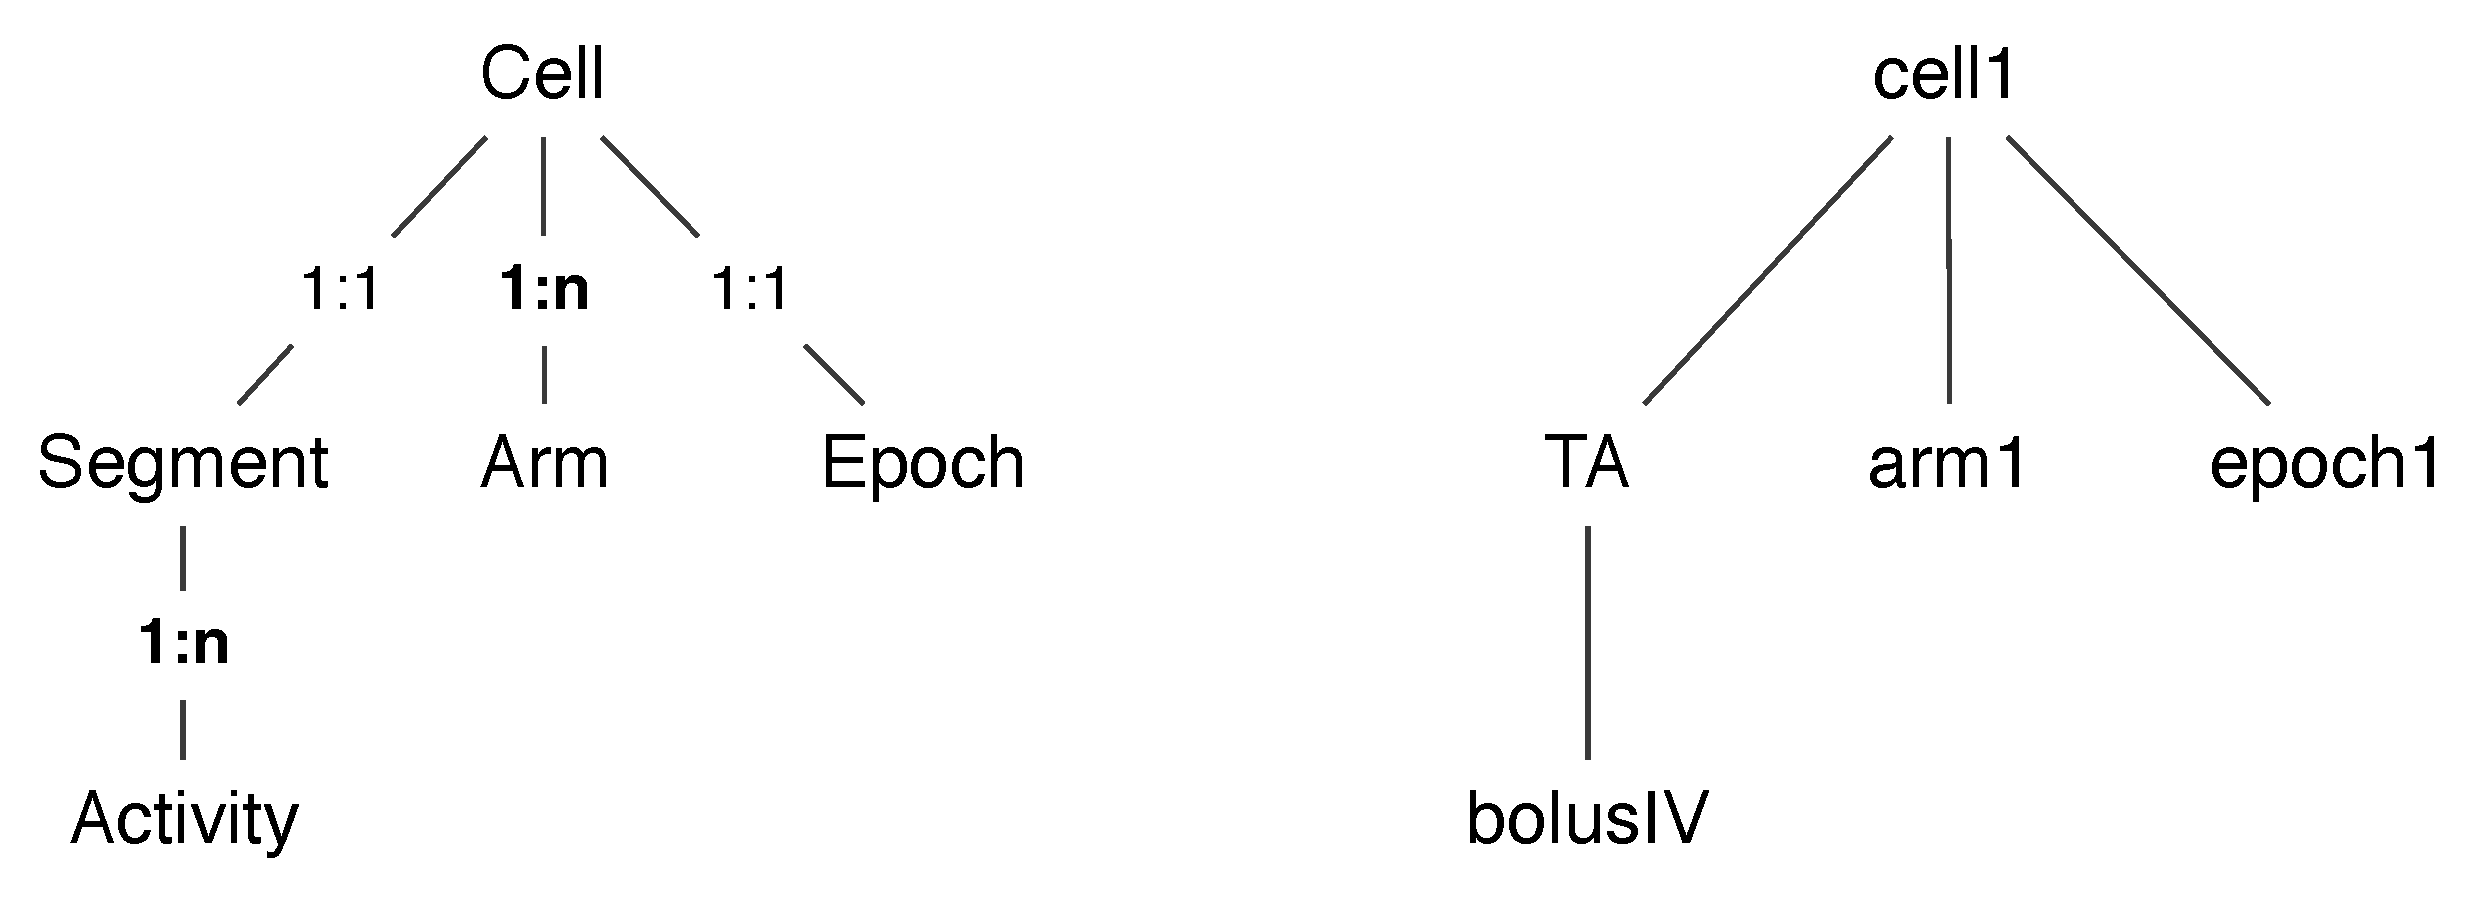
\includegraphics[width=0.7\linewidth]{pics/cellHierarchy_Ribba.pdf}
\caption{General cell hierarchy (left); The root of the trial design structure hierarchy is the 'Cell' which can contain one 'Segment',
one 'Epoch' and multiple 'Arms'. The 'Segment' element can have multiple child elements, the 'Activities', e.g. treatments or a washout. (right) An example of how it is applied in \cite{Ribba:2012uq}.}
\label{fig:cellHierarchy_Ribba}
\end{figure}

\begin{table}[htdp!]
\begin{center}
\begin{tabular}{ccccccc}
\hline
Segment&Activity & Treatment & DoseTime & DoseSize & Target Variable \\
\hline
TA& bolusIV &  IV bolus & individual & 1 & C \\
\hline
\end{tabular}
\end{center}
\caption{Segment/activity overview.}
\label{tab:segementActivity_Ribba}
\end{table}

%%%%%%%%%%%%%%%%%%%%%%%%%%%%%%%%%%%%%%%%%%%%%%%%%%%%%%%%%%%%%%%%
\subsubsection{Population}
In the next step, the \textit{Population} is defined, i.e. attributes of the individuals in the study. 
This means creating an individual template with columns for an identifier, arm and repetition and then
populating the table with appropriate data.
As no covariates are used here the \textit{Population} description reduces to the assignment 
of the subjects to the single study arm, \textit{Arm1}. As a shorthand we use the
\textit{repetition} method by defining the column 'rep', as can be seen in the following listing 
%\inputxml{Ribba_population.xml}
\lstset{language=XML}
\begin{lstlisting}
        <Population> 
            <ct:VariabilityReference>
                <ct:SymbRef blkIdRef="vm1" symbIdRef="indiv"/>
            </ct:VariabilityReference>
            
            <DataSet xmlns="http://www.pharmml.org/pharmml/0.6/Dataset">
                <Definition>
                    <Column columnId="ID" columnType="id" valueType="id" columnNum="1"/> 
                    <Column columnId="ARM" columnType="arm" valueType="id" columnNum="2"/> 
                    <Column columnId="REP" columnType="replicate" valueType="int" columnNum="3"/> 
                </Definition>
                <Table>
                    <Row>
                        <ct:Id>i</ct:Id>
                        <ct:Id>arm1</ct:Id>
                        <ct:Int>21</ct:Int>
                    </Row>
                </Table>
            </DataSet>
        </Population>
\end{lstlisting}

The identifiers, ID, created here are unique and will be used to the refer to specific subjects 
in the subsequent \xelem{IndividualDosing} structure element described in the following section.


%%%%%%%%%%%%%%%%%%%%%%%%%%%%%%%%%%%%%%%%%%%%%%%%%%%%%%%%%%%%%%%%
\subsubsection{Individual Dosing}
\label{subsubsec:Ribba_indivDosing}

This model utilises the idea of the so called K-PK model, meaning that the rate of the drug entry is relevant
but not its absolute value. Such models often assume, as it is the case here, that the dose is equal 1
for all subject and dosing events, see Table \ref{tab:example5_dataSet}.

The element \textit{IndividualDosing} is used to implementing all such subject specific
dosing events. First we have to associate the data which follow to an appropriate activity,
this is done by referring to the 'bolusIV' which defined previously in \xelem{Structure}, as 
as shown in the following listing 
%\inputxml{Ribba_individualDosing.xml}
\lstset{language=XML}
\begin{lstlisting}
        <IndividualDosing>
            <ActivityRef oidRef="bolusIV"/>
            <ColumnMapping>
                <ColumnRef xmlns="http://www.pharmml.org/pharmml/0.6/Dataset" columnIdRef="TIME"/>
                <ct:SymbRef symbIdRef="time"/>
            </ColumnMapping>
            <DataSet xmlns="http://www.pharmml.org/pharmml/0.6/Dataset">
                <Definition>
                    <Column columnId="ID" columnType="id" valueType="string" columnNum="1"/>
                    <Column columnId="TIME" columnType="idv" valueType="real" columnNum="2"/>
                    <Column columnId="DOSE" columnType="dose" valueType="real" columnNum="3"/>
                </Definition>
                <Table>
                    <!-- subject 1 -->
                    <Row><ct:String>1</ct:String><ct:Real>54.57</ct:Real><ct:Real>1</ct:Real></Row> 
                    <Row><ct:String>1</ct:String><ct:Real>59.77</ct:Real><ct:Real>1</ct:Real></Row> 
                    <!-- SNIP -->
                    <!-- subject 21 -->
                    <Row><ct:String>21</ct:String><ct:Real>1.5</ct:Real><ct:Real>1</ct:Real></Row> 
                    <Row><ct:String>21</ct:String><ct:Real>3.17</ct:Real><ct:Real>1</ct:Real></Row> 
                    <Row><ct:String>21</ct:String><ct:Real>4.85</ct:Real><ct:Real>1</ct:Real></Row> 
                    <Row><ct:String>21</ct:String><ct:Real>6.52</ct:Real><ct:Real>1</ct:Real></Row> 
                    <Row><ct:String>21</ct:String><ct:Real>8.19</ct:Real><ct:Real>1</ct:Real></Row> 
                    <Row><ct:String>21</ct:String><ct:Real>9.87</ct:Real><ct:Real>1</ct:Real></Row> 
                </Table>
            </DataSet>
        </IndividualDosing>
\end{lstlisting}

Next we map the subject's identifier \var{ID} to that created in the population definition. 
Finally a data set template using \xelem{Definition} element is defined, 
i.e. the columns \var{ID}, \var{TIME} and \var{DOSE}.
Then the table is populated with subject specific values as shown here for subjects 1, 2 and 21.


%%%%%%%%%%%%%%%%%%%%%%%%%%%%%%%%%%%%%%%%%%%%%%%%%%%%%%%%%%%%%%%%
\subsection{Structural model definition}
The following ODE system is defined:
\begin{align*}
\frac{dC}{dt} &= -\textit{KDE} \times C  \nonumber \\
\frac{dP}{dt} &= \lambda_P \times P \Big( 1 - \frac{P^\star}{K} \Big) + k_{\textit{QPP}} \times Q_P - k_{\textit{PQ}} \times P - \gamma \times C \times \textit{KDE} \times P  \nonumber \\
\frac{dQ}{dt} &= k_{PQ}\times P - \gamma \times C\times \mathit{KDE}\times Q \nonumber \\
\frac{dQ_P}{dt} &= \gamma \times C \times \textit{KDE} \times Q - k_{\textit{QPP}} \times Q_P - \delta_{\textit{QP}} \times Q_P  \nonumber \\ \nonumber \\
P^{\star} &= P + Q + Q_P \nonumber
\end{align*}
with initial conditions
\begin{align*}
C(t=0) = 1; \quad P(t=0) = P0; \quad Q(t=0) = Q0; \quad Q_P(t=0) = 0.  \nonumber
\end{align*}

%%%%%%%%%%%%%%%%%%%%%%%%%%%%%%%%%%%%%%%%%%%%%%%%%%%%%%%%%%%%%%%%
\subsubsection{Estimating initial conditions}
This example differs from the previous ones. It requires, in addition to model parameters, 
the estimation of the initial conditions of two tumour growth related variables. 
Moreover, the inter-individual variability is assumed for these variables.
The value for $Q_P(t=0)=Q_{P_0}$ is fixed to $0$ but the values for $P(t=0)=P_0$ and $Q(t=0)=Q_0$
are allowed to vary according to a log-normal distribution, see the following listing 
%\inputxml{Ribba_initialConditionsDef.xml} 
\lstset{language=XML}
\begin{lstlisting}
            <SimpleParameter symbId="pop_P0"/>
            <SimpleParameter symbId="omega_P0"/>
            <RandomVariable symbId="eta_P0">
                <ct:VariabilityReference>
                    <ct:SymbRef blkIdRef="vm1" symbIdRef="indiv"/>
                </ct:VariabilityReference>
                <NormalDistribution xmlns="http://www.uncertml.org/3.0" definition="">
                    <mean><rVal>0</rVal></mean>
                    <stddev><var varId="omega_P0"/></stddev>
                </NormalDistribution>
            </RandomVariable>
            <IndividualParameter symbId="P0">
                <GaussianModel>
                    <Transformation>log</Transformation>
                    <LinearCovariate>
                        <PopulationParameter>
                            <ct:Assign>
                                <ct:SymbRef symbIdRef="pop_P0"/>
                            </ct:Assign>
                        </PopulationParameter>
                    </LinearCovariate>
                    <RandomEffects>
                        <ct:SymbRef symbIdRef="eta_P0"/>
                    </RandomEffects>
                </GaussianModel>
            </IndividualParameter>            
\end{lstlisting}

where the definition of the distribution for the 
initial condition $P_0$ is shown.


%%%%%%%%%%%%%%%%%%%%%%%%%%%%%%%%%%%%%%%%%%%%%%%%%%%%%%%%%%%%%%%%
\subsection{NONMEM dataset}
\label{sec:eg5-NONMEMdataset}
Now we will describe the case when the data and trial design are sourced from the 
NONMEM dataset. Table \ref{tab:example4_dataSet} show a typical dataset required for 
an estimation task.
\begin{table}[htdp]
\begin{center}
\small
\begin{tabular}{rrrrrrrr}\toprule
ID	& TIME	& DV		& MDV	& AMT	& EVID \\ \midrule
1	& 0		& .		&  1		& .		& 0 \\
1	& 3.43	& 45.7	&  0		& .		& 0 \\
1	& 52.63	& 79.3	&  0		& .		& 0 \\
1	& 54.57	& .		&  1		& 1		& 1 \\
1	& 57.53	& 72.3	&  0		& .		& 0 \\
1	& 59.77	& .		&  1		& 1		& 1 \\
1	& 63.3	& 72.07	&  0		& .		& 0 \\
...	& ...		& ...		& ...		& ...		& ...  \\
1	& 121.87	& 90.16	&  0		& .		& 0 \\
2	& 0		& 50.17	&  0		& .		& 0 \\
2	& 12		& .		&  1		& 1		& 1 \\
2	& 14.09	& .		&  1		& 1		& 1 \\
2	& 14.17	& 52.82	&  0		& .		& 0 \\
...	& ...		& ...		& ...		& ...		& ... \\ \bottomrule
\end{tabular}
\end{center}
\caption{A dataset used in example \theexamples.
The columns are: the identifier, ID, time for measurements and dosing events, 
dependent variable, DV, which stands for \var{PSTAR} -- the total tumour size and 
the dose, DOSE. As common for K-PD models, the dose is equal 1 for all subjects and 
dosing events. }
\label{tab:example5_dataSet}
\end{table}%


The following code shows how the dataset definition and column mappings 
\lstset{language=XML}
\begin{lstlisting}
        <ExternalDataSet toolName="NONMEM" oid="NMoid">
            
            <ColumnMapping>
                <ColumnRef xmlns="http://www.pharmml.org/pharmml/0.6/Dataset" columnIdRef="ID"/>
                <ct:SymbRef blkIdRef="vm1" symbIdRef="indiv"/>
            </ColumnMapping>
            <ColumnMapping>
                <ColumnRef xmlns="http://www.pharmml.org/pharmml/0.6/Dataset" columnIdRef="TIME"/> 
                <ct:SymbRef symbIdRef="time"/>
            </ColumnMapping>
            <ColumnMapping>
                <ColumnRef xmlns="http://www.pharmml.org/pharmml/0.6/Dataset" columnIdRef="DV"/> 
                <ct:SymbRef blkIdRef="om1" symbIdRef="PSTAR_obs"/>
            </ColumnMapping>
            <ColumnMapping>
                <ColumnRef xmlns="http://www.pharmml.org/pharmml/0.6/Dataset" columnIdRef="AMT"/>
                <ct:SymbRef blkIdRef="om1" symbIdRef="C"/>
            </ColumnMapping>
            
            <!--columns: ID TIME DV MDV DOSE EVID-->
            <DataSet xmlns="http://www.pharmml.org/pharmml/0.6/Dataset">
                <Definition>
                    <Column columnId="ID" columnType="id" valueType="string" columnNum="1"/>
                    <Column columnId="TIME" columnType="time" valueType="real" columnNum="2"/>
                    <Column columnId="DV" columnType="dv" valueType="real" columnNum="3"/>
                    <Column columnId="MDV" columnType="mdv" valueType="int" columnNum="4"/>
                    <Column columnId="AMT" columnType="dose" valueType="real" columnNum="5"/>
                    <Column columnId="EVID" columnType="evid" valueType="int" columnNum="6"/>
                </Definition>
                <ImportData oid="dataOid">
                    <path>datasets/example5.csv</path>
                    <format>CSV</format>
                    <delimiter>COMMA</delimiter>
                </ImportData>
            </DataSet>
        </ExternalDataSet>
\end{lstlisting}


%%%%%%%%%%%%%%%%%%%%%%%%%%%%%%%%%%%%%%%%%%%%%%%%%%%%%%%%%%%%%%%%
\subsection{Modelling steps}
This requires the specification of the following items: \textit{EstimationStep} and \textit{StepDependencies}.
It has been described in previous examples in detail and will be skipped here.


%%%%%%%%%%%%%%%%%%%%%%%%%%%%%%%%%%%%%%%%%%%%%%%%%%%%%%%%%%%%%%%%
%%%%%%%%%%%%%%%%%%%%%%%%%%%%%%%%%%%%%%%%%%%%%%%%%%%%%%%%%%%%%%%%
%%%%%%%%%%%%%%%%%%%%%%%%%%%%%%%%%%%%%%%%%%%%%%%%%%%%%%%%%%%%%%%%

\eglabel{6}
\section{Example \theexamples: Joint PKPD model with count data}
\label{sec:eg6}
The following three examples features a new aspect of the \pml, the support of discrete 
data models\footnote{The discrete data models are coming in a large variety, which 
would be worth a detailed discussion. This and the next examples can cover, for 
the sake of space, only the very basic cases. More examples, encoded completely 
in \pml, can be found on our webpage \url{http://pharmml.org}. See also discrete data 
model templates in the appendix, \ref{chapter:codeTemplates}.}. The first one is using 
the Poisson distribution to describe count data\footnote{The example is encoded 
in \xatt{example6\_NONMEM.xml} with design sourced from a NONMEM datafile.}, 
from the MLXTRAN tutorial, \cite{Monolix4.3Tutorial:2014}.
%%%%%%%%%%%%%%%%%%%%%%%%%%%%%%%%%%%%%%%%%%%%%%%%%%%%%%%%%%%%%%%%
\subsection{Description}
\label{subsec:exp6_intro}
 
The essential bit of information for this task is the probability distribution, the probability 
mass function (PMF), of count data Y, which can be defined in either un-transformed, 
P(Y=k), or transformed, log(P(Y=k)), form. As in example \ref{sec:eg1}, the underlying 
PK model is 1-compartmental oral model and will be omitted here. We assume the basic 
Poisson model which reads
\begin{eqnarray}
&& P\big(Y_{\iijj}=k | \Cc_{\iijj}, \psi_i\big) =  \frac{e^{-\lambda_{\iijj}} \lambda^k_{\iijj}}{k!} \label{eq:poissonModel}
\end{eqnarray}
with concentration dependent mean $\lambda$, defined as
\begin{eqnarray}
&& \lambda_{\iijj} = \lambda_0 \Big(1 - \frac{\Cc_{\iijj}}{IC_{50} + \Cc_{\iijj}}\Big)  \label{eq:lambdasurface}
\end{eqnarray}
\begin{figure}[htbp]
\centering
%\begin{tabular}{cc}
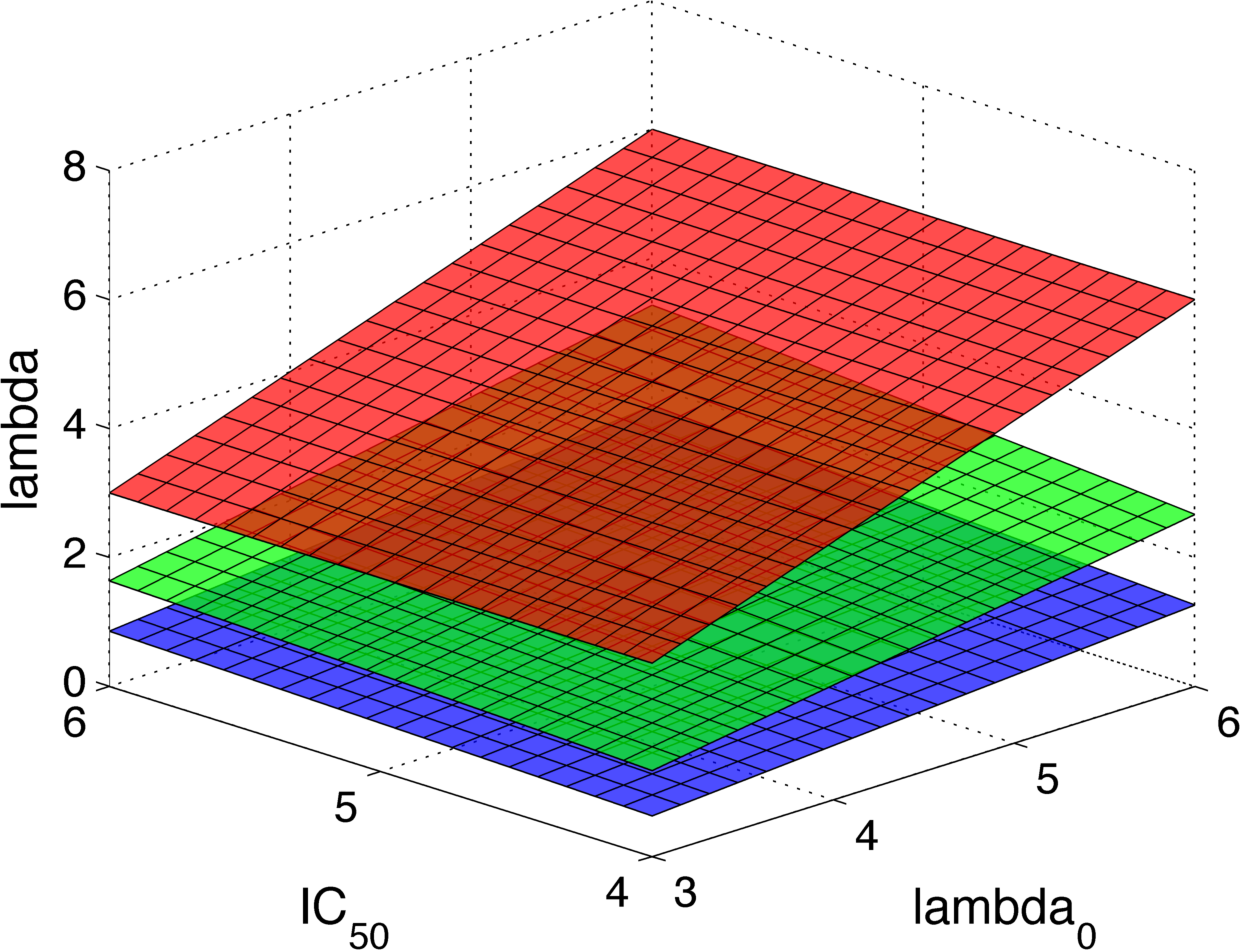
\includegraphics[width=.43\textwidth]{pics/CTS4_lambda_threeSurfaces} 
%& \raisebox{0\height}{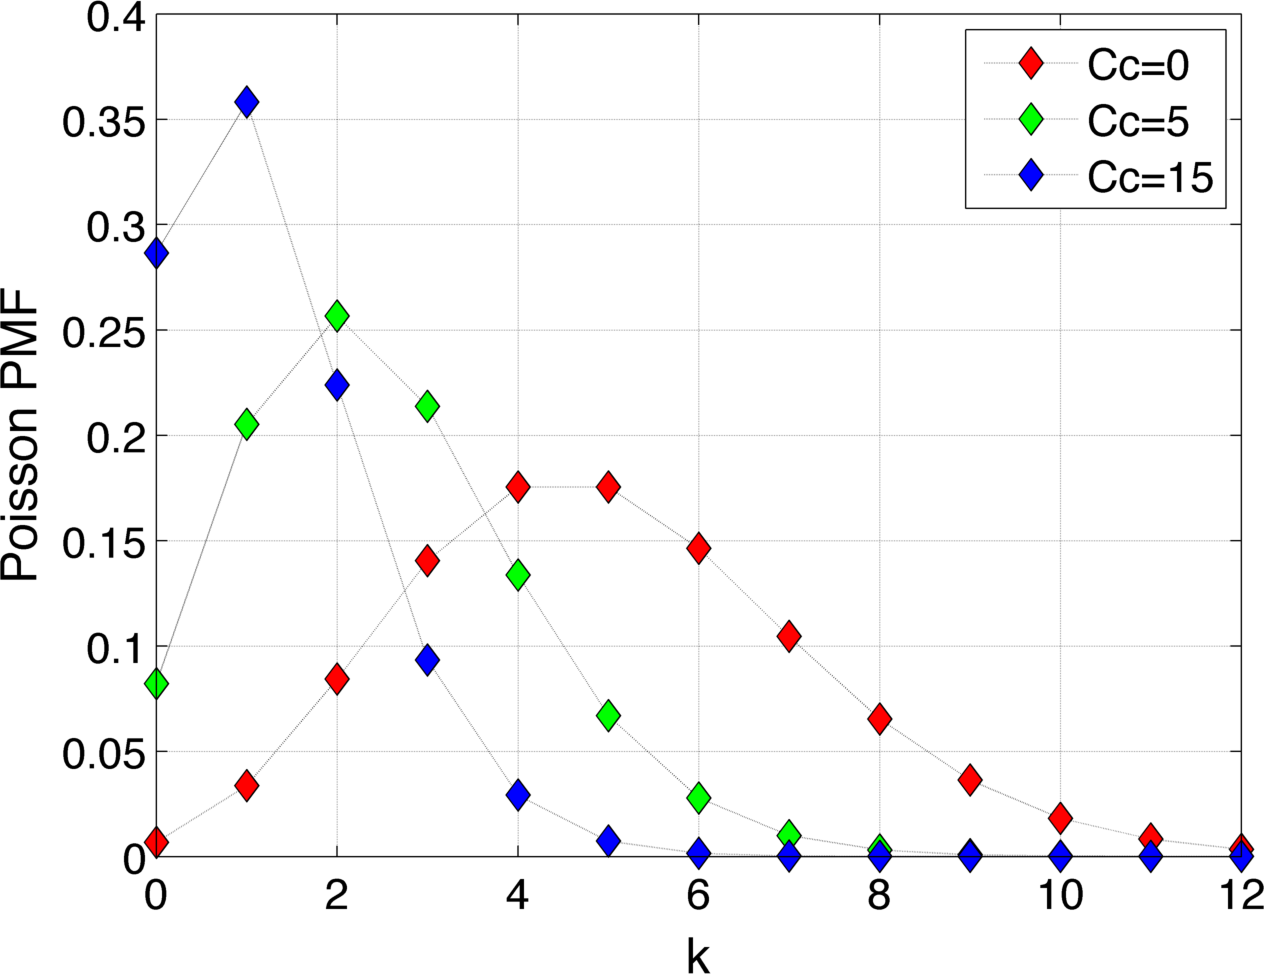
\includegraphics[scale=0.45]{pics/CTS4_poissonScan}}
%\end{tabular}
\caption{$\lambda$--surface as function of $\lambda_0$ and $IC_{50}$ 
plotted for $\Cc = \{1,5,15\}$.}
\label{fig:lambdasurface}
\end{figure}
also called \emph{Poisson intensity}. Here, $\lambda$, depends on the parameters 
$\lambda_0$ and $IC_{50}$ which are sampled from log-normal distribution. 
$\lambda_0$, stands here for the baseline seizure count prior to any drug. 
The value of $\lambda$ is reduced by the concentration in the central 
compartment, $\Cc$, which is visualised for three different values 
of $\Cc = \{1,5,15\}$ in \ref{fig:lambdasurface} ($1\equiv$ green, $5 \equiv$ 
red, $15 \equiv$ blue).


\begin{figure}[ht!]
\centering
\begin{tabular}{cc}
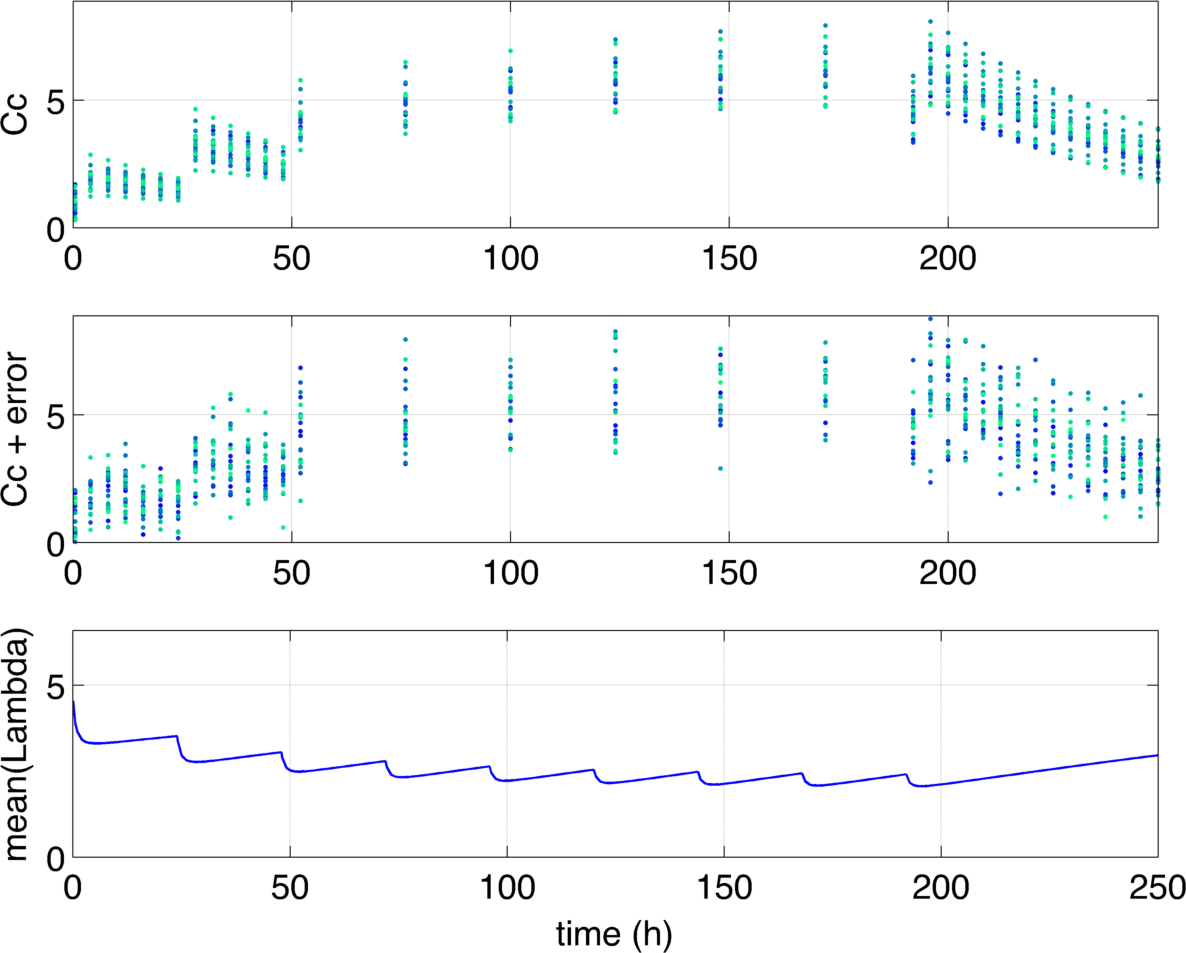
\includegraphics[width=.49\textwidth]{pics/CTS4_PK_meanLambda_armB} & 
\raisebox{0.05\height}{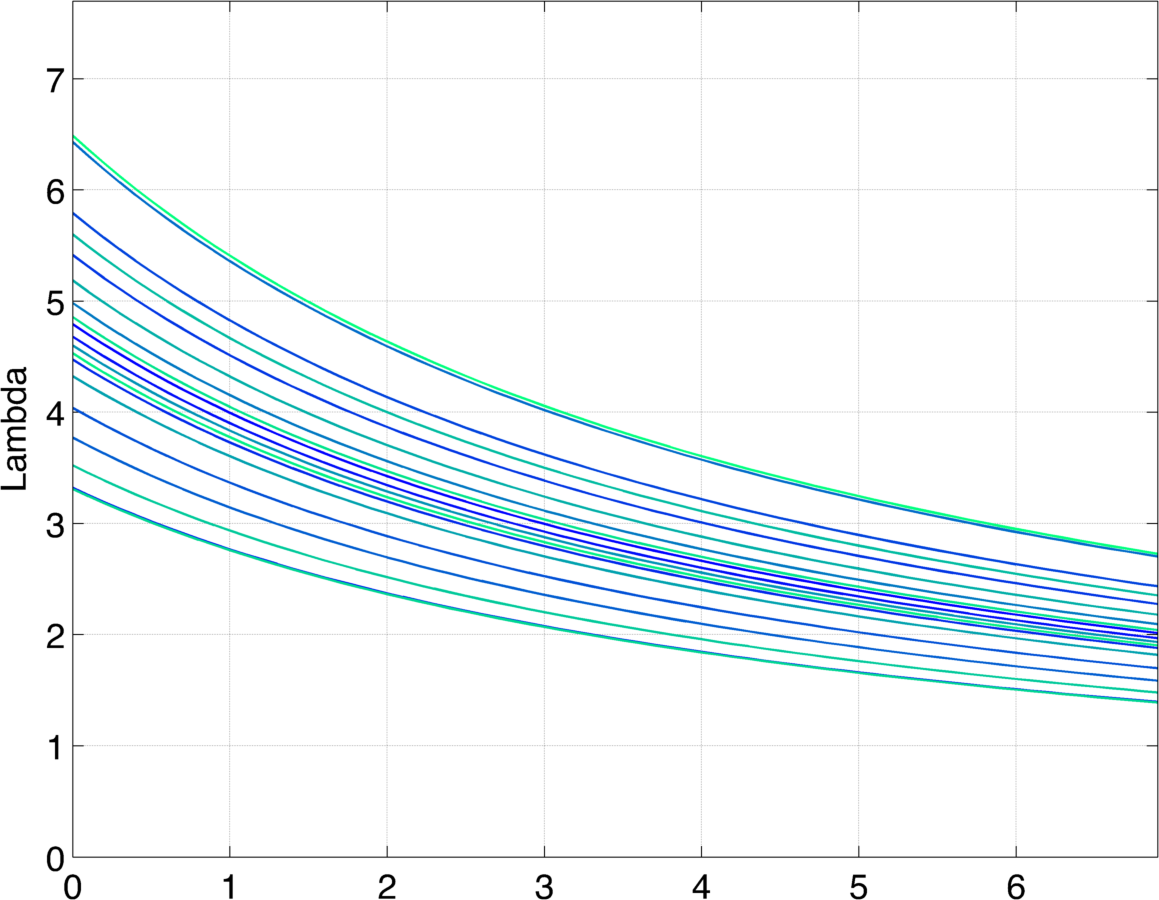
\includegraphics[scale=0.4875]{pics/CTS4_lambda}}
\end{tabular}
\caption{(left) The time courses for the concentration and mean Poisson intensity, $\lambda$. 
(right) Poisson intensity as given by eq.(\ref{eq:lambdasurface}) for all subject 
as function of the concentration between 0 and the maximum achievable 
concentration across 20 subjects.}
\label{fig:lambdaTiemCourse}
\end{figure}

\subsubsection{Individual parameters model}
\begin{eqnarray}
\lambda_0 & \sim&  \mbox{logNormal}(\pop_{\lambda_0}, \omega_{\lambda_0}); \quad  \pop_{\lambda_0} = 5, \quad \omega_{\lambda_0} = 0.2 \nonumber \\
IC_{50} &\sim& \mbox{logNormal}(\pop_{IC_{50}}, \omega_{IC_{50}}); \quad  \pop_{IC_{50}} = 5, \quad \omega_{IC_{50}} = 0 \nonumber
\end{eqnarray}


\subsubsection{Observation model}
We apply a combined residual error model to the continuous PK output variable 
\var{Cc} and Poisson error distribution for the discrete PD component, defined by \var{Y}, 
as the following table shows 

%\begin{table*}[h!]
\begin{center}
\small
\renewcommand{\arraystretch}{1.1}% 
\begin{tabular*}{0.8\linewidth}{@{\extracolsep{\fill}} >{\bfseries}l l l}\toprule
Output Variable & \textbf{\itshape Cc} &\textbf{\itshape Y}\\\midrule
Observation Name & Concentration & State \\
Units & $\mg/l$ & -- \\
Type & Continuous & Discrete/Count \\
Model & Combined & Poisson\\
Parameters 	& $a, b$ 	& $\lambda_0, IC_{50}$\\
%Regressor	& --		& $Cc$ \\
\bottomrule
\end{tabular*}
\end{center}
Two additional important bits of information which are part of the discrete observation
mode to be provided are 
\begin{itemize}
\item
Intensity Parameter, $\lambda$, given by eq. (\ref{eq:lambdasurface})
\item
Link function -- $\log$.
\end{itemize}

%%%%%%%%%%%%%%%%%%%%%%%%%%%%%%%%%%%%%%%%%%%%%%%%%%%%%%%%%%%%%%%%
\subsubsection{Modelling Steps}

The PK and PD output variables to be generated by the simulation and
their associated time points are shown below:

\begin{center}
\small
\renewcommand{\arraystretch}{1.1}% 
\begin{tabular*}{0.9\linewidth}{@{\extracolsep{\fill}} >{\bfseries}l c c}\toprule
Output Variable & \textbf{\itshape Cc} &\textbf{\itshape $\lambda$}\\\midrule
Observation times & [0.5,4 : 4 : 48, 52 : 24 : 192, 192 : 4 : 250] & 0 : 24 : 192\\
\bottomrule
\end{tabular*}
\end{center}


%%%%%%%%%%%%%%%%%%%%%%%%%%%%%%%%%%%%%%%%%%%%%%%%%%%%%%%%%%%%%%%%
\subsection{Observation model}
While the continuous observation model and its features as applied for example 
for the concentration have been described in very detail in the previous examples,
the error distribution of the discrete effect given by eqs.(\ref{eq:poissonModel}) 
and (\ref{eq:lambdasurface}) will be described in the following for the first time.

First we have to indicate the type of the observation model using the elements 
\xelem{Discrete} and specifically for this example the \xelem{CountData}. The next 
mandatory elements are the count index, \emph{k}, (required only when the PMF is 
explicitly specified, see below) and the \xelem{CountVariable} which will be used later
to establish the link between the model and the related date set, see Table 
\ref{tab:example6_dataSet}.
Then the characteristic parameter for the Poisson distribution is implemented, 
the \emph{Poisson intensity}, $\lambda$, as function of the drug concentration, $Cc$.

\lstset{language=XML}
\begin{lstlisting}
        <ObservationModel blkId="om1">
            <Discrete>
                <CountData>
                    <ct:Variable symbolType="int" symbId="k"/>
                    <CountVariable symbId="Y"/>
                    
                    <!-- Poisson intensity - function of drug concentration, Cc -->                    
                    <IntensityParameter symbId="Lambda">
                        <ct:Assign>
                            <math:Equation>
                                <math:Binop op="times">
                                    <ct:SymbRef blkIdRef="pm1" symbIdRef="lambda0"/>
                                    <math:Binop op="minus">
                                        <ct:Real>1</ct:Real>
                                        <math:Binop op="divide">
                                            <ct:SymbRef blkIdRef="sm1" symbIdRef="Cc"/>
                                            <math:Binop op="plus">
                                                <ct:SymbRef blkIdRef="pm1" symbIdRef="IC50"/>
                                                <ct:SymbRef blkIdRef="sm1" symbIdRef="Cc"/>
                                            </math:Binop>
                                        </math:Binop>
                                    </math:Binop>
                                </math:Binop>
                            </math:Equation>
                        </ct:Assign>
                    </IntensityParameter>
                    <!-- see next listing for the continuation of the observation model -->
\end{lstlisting}
Now the Poisson probability mass function (PMF) can be defined, but here 
in the transformed format 
\begin{align}
\log(P\big(Y_{\iijj} & =k | \Cc_{\iijj}, \psi_i\big)) =  -\lambda_{\iijj} +k\times \lambda_{\iijj} - \log(k!) \nonumber
\end{align}
which can be done in various ways, either
\begin{itemize}
\item
using the UncertML standard as in the following snippet
\lstset{language=XML}
\begin{lstlisting}
                    <PMF linkFunction="log">
                        <PoissonDistribution xmlns="http://www.uncertml.org/3.0" 
                            definition="http://www.uncertml.org/3.0">
                            <rate>
                                <var varId="Lambda"/>
                            </rate>
                        </PoissonDistribution>
                    </PMF>
                </CountData>
            </Discrete>
        </ObservationModel>
\end{lstlisting}
\item
by encoding explicitly the PMF in the transformed format and specifying the
the applied link function, here the logarithm, as the following snippet shows
\lstset{language=XML}
\begin{lstlisting}
                    <PMF linkFunction="log">
                        <math:LogicBinop op="eq">
                            <ct:SymbRef symbIdRef="Y"/>
                            <ct:SymbRef symbIdRef="k"/>
                        </math:LogicBinop>
                        <ct:Assign>
                            <Equation xmlns="http://www.pharmml.org/pharmml/0.6/Maths">
                                <Binop op="minus">
                                    <Binop op="plus">
                                        <Uniop op="minus">
                                            <ct:SymbRef symbIdRef="Lambda"/>
                                        </Uniop>
                                        <Binop op="times">
                                            <ct:SymbRef symbIdRef="k"/>
                                            <Uniop op="log">
                                                <ct:SymbRef symbIdRef="Lambda"/>
                                            </Uniop>
                                        </Binop>
                                    </Binop>
                                    <Uniop op="factln">
                                        <ct:SymbRef symbIdRef="k"/>
                                    </Uniop>
                                </Binop>
                            </Equation>
                        </ct:Assign>
                    </PMF>
                </CountData>
            </Discrete>
        </ObservationModel> 
\end{lstlisting}
\end{itemize}

Note, that although the UncertML driven solution is very simple and straightforward
to implement, it is also limited to only this case, see also Section \ref{subsec:DiscreteData}. 
In short, for count data models, only the basic Poisson model is available in the UncertML standard.


%%%%%%%%%%%%%%%%%%%%%%%%%%%%%%%%%%%%%%%%%%%%%%%%%%%%%%%%%%%%%%%%
\subsection{NONMEM dataset}
\label{sec:eg6-NONMEMdataset}
The remaining part is the the data and trial design as sourced from the 
NONMEM dataset. Table \ref{tab:example6_dataSet} show a typical dataset required for 
an estimation task.
\begin{table}[htdp]
\begin{center}
\small
\renewcommand{\arraystretch}{1.1}% 
\begin{tabular}{rrrrrrrr}\toprule
ID 	& TIME	& AMT	& Y		& DVID \\ \midrule
1 	& 0 		& 100 	& . 		& . \\ 
1 	& 4 		& . 		& 9.2 	& 1 \\ 
1 	& 8 		& . 		& 5 		& 2 \\ 
1 	& 12 	& . 		& 8.5 	& 1 \\ 
1 	& 18 	& . 		& 6.4 	& 1 \\ 
1 	& 24 	& . 		& 2 		& 2 \\ 
2 	& 0 		& 120	&  26 	& . \\ 
2 	& 4 		& . 		& 4.8 	& 1 \\ 
2 	& 8 		& . 		& 3 		& 2 \\ 
2 	& 12 	& . 		& 3.1 	& 1 \\ 
2 	& 18 	& . 		& 2.5 	& 1 \\ 
2 	& 24 	& . 		& 0 		& 2 \\ 
...	& ...		& ...		& ...		& ...	\\ \bottomrule
\end{tabular}
\end{center}
\caption{A dataset used in example for first two subjects.
The additional column DVID is used to specify the type of data. Here, 
DVID =1 is used for a continuous response and DVID =2 for count data.}
\label{tab:example6_dataSet}
\end{table}%

\lstset{language=XML}
\begin{lstlisting}
        <mstep:ExternalDataSet toolName="NONMEM" oid="NMoid">
            <mstep:ColumnMapping>
                <ds:ColumnRef columnIdRef="TIME"/>
                <ct:SymbRef symbIdRef="t"/>
            </mstep:ColumnMapping>
            <mstep:ColumnMapping>
                <ds:ColumnRef columnIdRef="AMT"/>
                <ct:SymbRef blkIdRef="sm1" symbIdRef="Ad"/>
            </mstep:ColumnMapping>
            <mstep:MultipleDVMapping>
                <ds:ColumnRef columnIdRef="DV"/>
                <mstep:Piecewise>
                    <math:Piece>
                        <ct:SymbRef blkIdRef="om1" symbIdRef="Y"/>
                        <math:Condition>
                            <math:LogicBinop op="eq">
                                <ds:ColumnRef columnIdRef="DVID"/>
                                <ct:Int>2</ct:Int>
                            </math:LogicBinop>
                        </math:Condition>
                    </math:Piece>
                    <math:Piece>
                        <ct:SymbRef blkIdRef="om2" symbIdRef="Cc_obs"/>
                        <math:Condition>
                            <math:LogicBinop op="eq">
                                <ds:ColumnRef columnIdRef="DVID"/>
                                <ct:Int>1</ct:Int>
                            </math:LogicBinop>
                        </math:Condition>
                    </math:Piece>
                </mstep:Piecewise>
            </mstep:MultipleDVMapping>
            <ds:DataSet>
                <ds:Definition>
                    <ds:Column columnId="ID" columnType="id" valueType="string" columnNum="1"/>
                    <ds:Column columnId="TIME" columnType="idv" valueType="real" columnNum="2"/>
                    <ds:Column columnId="AMT" columnType="dose" valueType="real" columnNum="3"/>
                    <ds:Column columnId="DV" columnType="dv" valueType="real" columnNum="4"/>
                    <ds:Column columnId="DVID" columnType="dvid" valueType="real" columnNum="5"/>
                </ds:Definition>
                <ds:ExternalFile oid="dataOid">
                    <ds:path>datasets/example_poisson.csv</ds:path>
                </ds:ExternalFile>
            </ds:DataSet>
        </mstep:ExternalDataSet>
\end{lstlisting}

Mapping of dosing related data has been described previously on
multiple occasions and will not be discussed here. The conditional mapping required 
in the case when multiple observations have to be mapped using the \xelem{mstep:MultipleDVMapping}
has been described in example 1, see section \ref{sec:eg1-NONMEMdataset}. 
What is new however is the mapping target when dealing with count data.
The count variable, \emph{Y}, as defined in the very beginning of the \xelem{CountData} 
in the observation model \xatt{om1} as the snippet shows
\lstset{language=XML}
\begin{lstlisting}
		<CountVariable symbId="Y"/>
\end{lstlisting}
is the target for this mapping and is conditional on the value of the column \emph{DVID}.




%%%%%%%%%%%%%%%%%%%%%%%%%%%%%%%%%%%%%%%%%%%%%%%%%%%%%%%%%%%%%%%%
%%%%%%%%%%%%%%%%%%%%%%%%%%%%%%%%%%%%%%%%%%%%%%%%%%%%%%%%%%%%%%%%
%%%%%%%%%%%%%%%%%%%%%%%%%%%%%%%%%%%%%%%%%%%%%%%%%%%%%%%%%%%%%%%%

\newpage

\eglabel{7}
\section{Example \theexamples: Joint PKPD model with categorical data}
\label{sec:eg7}

%%%%%%%%%%%%%%%%%%%%%%%%%%%%%%%%%%%%%%%%%%%%%%%%%%%%%%%%%%%%%%%%
\subsection{Description}
\label{subsec:exp7_intro} 
The following example features another type of discrete models supported by \pml -- 
the categorical data models.

In this example, there are two categories, $k \in {0,1}$, i.e. the effect outcome is either 0 or 1. 
The underlying PK model is again an 1-compartmental oral model and will no t be described. 
The probability for the category 1 is given by the following formula 
\begin{eqnarray}
	p1 &=& \frac{1}{1+\exp(-\theta_1 - \theta_2 \log(\Cc))} 	\label{eq:p1surface}
\end{eqnarray}
which is plotted in \ref{fig:p1surface}. This $p1$--surface is also function of $\theta_1$, 
$\theta_2$ and $log(\Cc)$ which is visualised for three different values of $\Cc = \{1,5,15\}$. 

\begin{figure}[htbp]
\begin{center}
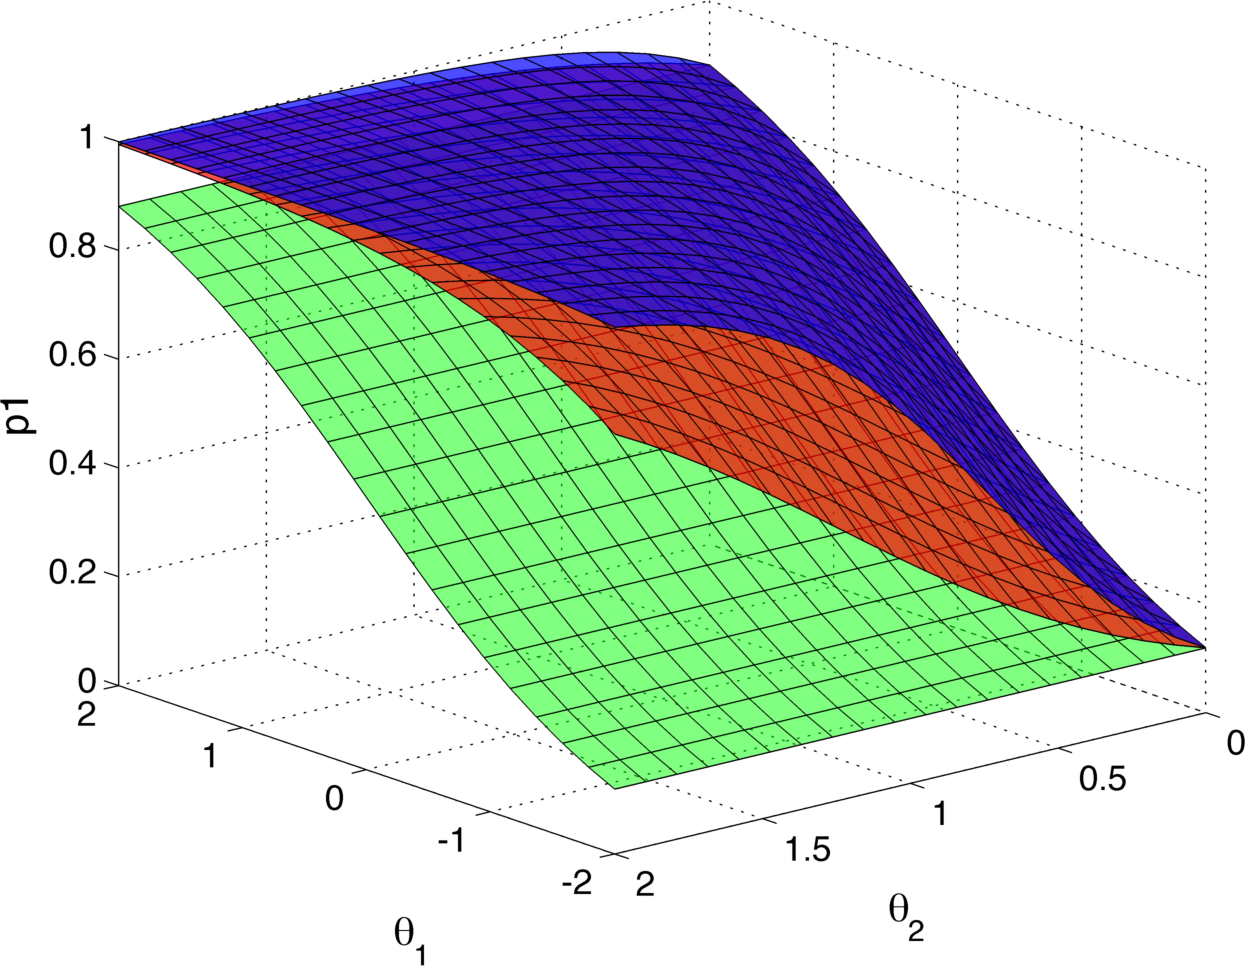
\includegraphics[width=.45\textwidth]{pics/p1_threeSurfaces.png}
\caption{p1 probability surface as function of $\theta_1$ and $\theta_2$ plotted for 
Cc = \{1,5,15\} ($1\equiv$ green, $5 \equiv$ red, $15 \equiv$ blue). }
\label{fig:p1surface}
\end{center}
\end{figure}

\subsubsection{Individual parameters model}
\begin{eqnarray}
theta1& \sim&  \mbox{Normal}(\pop_{theta1}, \omega_{theta1}); \quad \pop_{theta1}=-1,\quad \omega_{theta1}=0.3 \nonumber \\
theta2& \sim&  \mbox{logNormal}(\pop_{theta2}, \omega_{theta2}); \quad \pop_{theta2}=1,\quad \omega_{theta2}=0.2 \nonumber 
\end{eqnarray}

\subsubsection{Observation model}
We apply a combined residual error model to the continuous PK output variable 
\var{Cc} and Poisson error distribution for the discrete PD component, defined by \var{Y}, 
as the following table shows 

%\begin{table*}[h!]
\begin{center}
\small
\renewcommand{\arraystretch}{1.1}% 
\begin{tabular*}{0.8\linewidth}{@{\extracolsep{\fill}} >{\bfseries}l l l}\toprule
Output Variable & \textbf{\itshape Cc} &\textbf{\itshape Y}\\\midrule
Observation Name & Concentration & State \\
Units & $\mg/l$ & -- \\
Type & Continuous & Discrete/Categorical \\
Model & Combined & Binomial\\
Parameters 	& $a, b$ 	& $\theta_1$, $\theta_2$\\
%Regressor	& --		& $Cc$ \\
\bottomrule
\end{tabular*}
\end{center}

%%%%%%%%%%%%%%%%%%%%%%%%%%%%%%%%%%%%%%%%%%%%%%%%%%%%%%%%%%%%%%%%
\subsubsection{Modelling Steps}

The PK and PD output variables to be generated by the simulation and
their associated time points are shown below:

\begin{center}
\small
\renewcommand{\arraystretch}{1.1}% 
\begin{tabular*}{0.9\linewidth}{@{\extracolsep{\fill}} >{\bfseries}l c c}\toprule
Output Variable & \textbf{\itshape Cc} &\textbf{\itshape $p1$}\\\midrule
Observation times & [0.5,4 : 4 : 48, 52 : 24 : 192, 192 : 4 : 250] & 0 : 24 : 288\\
\bottomrule
\end{tabular*}
\end{center}


\begin{figure}[htbp]
\centering
\begin{tabular}{cc}
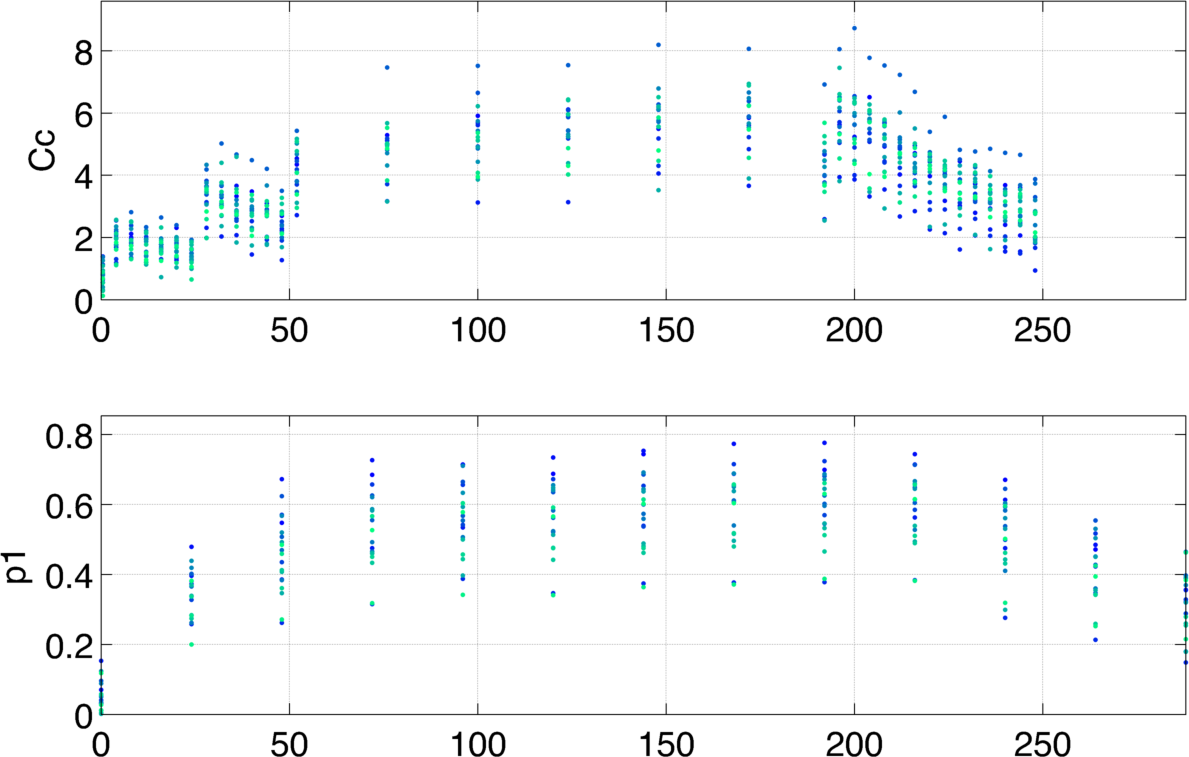
\includegraphics[width=.6\textwidth]{pics/p1_armA} 
\end{tabular}
\caption{Plots for first arm in the study. (top) Concentration, \emph{Cc}, time course of the PK model. 
(bottom) Probability, \emph{p1}, time course as defined in eq.\ref{eq:p1surface}.}
\label{fig:lambdasurface}
\end{figure}


%%%%%%%%%%%%%%%%%%%%%%%%%%%%%%%%%%%%%%%%%%%%%%%%%%%%%%%%%%%%%%%%
\subsection{Observation model}

\lstset{language=XML}
\begin{lstlisting}
        <ObservationModel blkId="om1">
            <Discrete>
                <CategoricalData ordered="no">
                    
                    <ct:Variable symbolType="real" symbId="p1">
                        <ct:Assign>
                            <math:Equation>
                                <math:Binop op="divide">
                                    <ct:Real>1</ct:Real>
                                    <math:Binop op="plus">
                                        <ct:Real>1</ct:Real>
                                        <math:Uniop op="exp">
                                            <math:Binop op="minus">
                                                <math:Uniop op="minus">
                                                    <ct:SymbRef blkIdRef="pm1" symbIdRef="theta1"/>
                                                </math:Uniop>
                                                <math:Binop op="times">
                                                    <ct:SymbRef blkIdRef="pm1" symbIdRef="theta2"/>
                                                    <math:Uniop op="log">
                                                        <ct:SymbRef blkIdRef="sm1" symbIdRef="Cc"/>
                                                    </math:Uniop>
                                                </math:Binop>
                                            </math:Binop>
                                        </math:Uniop>
                                    </math:Binop>
                                </math:Binop>
                            </math:Equation>                            
                        </ct:Assign>
                    </ct:Variable>
                    
                    <ListOfCategories> 
                        <Category symbId="cat0"/>
                        <Category symbId="cat1"/>
                    </ListOfCategories>
                    
                    <CategoryVariable symbId="y"/>
                    
                    <PMF linkFunction="identity">
                        <BinomialDistribution xmlns="http://www.uncertml.org/3.0" definition="">
                            <numberOfTrials>
                                <nVal>1</nVal>
                            </numberOfTrials>
                            <probabilityOfSuccess>
                                <var varId="p1"/>
                            </probabilityOfSuccess>
                        </BinomialDistribution>
                    </PMF>
                </CategoricalData>
            </Discrete>
        </ObservationModel>
\end{lstlisting}

%%%%%%%%%%%%%%%%%%%%%%%%%%%%%%%%%%%%%%%%%%%%%%%%%%%%%%%%%%%%%%%%
\subsection{NONMEM dataset}
\label{sec:eg7-NONMEMdataset}
The remaining part is the the data and trial design as sourced from the 
NONMEM dataset. Table \ref{tab:example7_dataSet} show a typical dataset required for 
an estimation task.
\begin{table}[htdp]
\begin{center}
\small
46	1	1
46	2	0
46	3	0
46	4	0
47	1	0
47	2	0
47	3	0
47	4	3
48	1	0
48	2	1
48	3	2
48	4	0
49	1	0
\renewcommand{\arraystretch}{1.1}% 
\begin{tabular}{rrrrrrrr}\toprule
ID 	& TIME	& AMT	& Y		& DVID \\ \midrule
1 	& 0 		& 100 	& . 		& . \\ 
1 	& 1 		& . 		& 1	 	& 2 \\ 
1 	& 4 		& . 		& 9.2 	& 1 \\ 
1 	& 8 		& . 		& 0 		& 2 \\ 
1 	& 10		& . 		& 0	 	& 2 \\ 
1 	& 12 	& . 		& 8.5 	& 1 \\ 
1 	& 18 	& . 		& 6.4 	& 1 \\ 
1 	& 24 	& . 		& 1 		& 2 \\ 
2 	& 0 		& 120	&  26 	& . \\ 
2 	& 4 		& . 		& 4.8 	& 1 \\ 
2 	& 8 		& . 		& 0 		& 2 \\ 
2 	& 12 	& . 		& 3.1 	& 1 \\ 
2 	& 18 	& . 		& 2.5 	& 1 \\ 
2 	& 24 	& . 		& 1 		& 2 \\ 
...	& ...		& ...		& ...		& ...	\\ \bottomrule
\end{tabular}
\end{center}
\caption{A dataset used in example for first two subjects.
The additional column DVID is used to specify the type of data. Here, 
DVID =1 is used for a continuous response and DVID =2 for count data.}
\label{tab:example7_dataSet}
\end{table}%

%%%%%%%%%%%%%%%%%%%%%%%%%%%%%%%%%%%%%%%%%%%%%%%%%%%%%%%%%%%%%%%%
\subsubsection{'Nested' mapping}

\lstset{language=XML}
\begin{lstlisting}
        <mstep:ExternalDataSet toolName="NONMEM" oid="NMoid">
            
            <mstep:ColumnMapping>
                <ds:ColumnRef columnIdRef="TIME"/>
                <ct:SymbRef symbIdRef="t"/>
            </mstep:ColumnMapping>
            <mstep:ColumnMapping>
                <ds:ColumnRef columnIdRef="AMT"/>
                <ct:SymbRef blkIdRef="sm1" symbIdRef="Ad"/>
            </mstep:ColumnMapping>
            <mstep:MultipleDVMapping>
                <ds:ColumnRef columnIdRef="DV"/>
                <mstep:Piecewise>
                    <math:Piece>
                        <ct:SymbRef blkIdRef="om1" symbIdRef="y"/>
                        <math:CategoryMapping>
                            <ds:Map dataSymbol="0" modelSymbol="cat0"/>
                            <ds:Map dataSymbol="1" modelSymbol="cat1"/>
                        </math:CategoryMapping>
                        <math:Condition>
                            <math:LogicBinop op="eq">
                                <ds:ColumnRef columnIdRef="DVID"/>
                                <ct:Int>2</ct:Int>
                            </math:LogicBinop>
                        </math:Condition>
                    </math:Piece>
                    <math:Piece>
                        <ct:SymbRef blkIdRef="om2" symbIdRef="C_obs"/>
                        <math:Condition>
                            <math:LogicBinop op="eq">
                                <ds:ColumnRef columnIdRef="DVID"/>
                                <ct:Int>1</ct:Int>
                            </math:LogicBinop>
                        </math:Condition>
                    </math:Piece>
                </mstep:Piecewise>
            </mstep:MultipleDVMapping>
            
            <!-- Dataset omitted, identical as in previous example -->
        </mstep:ExternalDataSet>
\end{lstlisting}



%%%%%%%%%%%%%%%%%%%%%%%%%%%%%%%%%%%%%%%%%%%%%%%%%%%%%%%%%%%%%%%%
%%%%%%%%%%%%%%%%%%%%%%%%%%%%%%%%%%%%%%%%%%%%%%%%%%%%%%%%%%%%%%%%
%%%%%%%%%%%%%%%%%%%%%%%%%%%%%%%%%%%%%%%%%%%%%%%%%%%%%%%%%%%%%%%%

\newpage

\eglabel{8}
\section{Example \theexamples: Joint PKPD model with Time-to-event effect}
\label{sec:eg8}

%%%%%%%%%%%%%%%%%%%%%%%%%%%%%%%%%%%%%%%%%%%%%%%%%%%%%%%%%%%%%%%%
\subsection{Description}
\label{subsec:exp8_intro} 
Time-to-effect is yet another type of discrete models supported by \pml, see Section 
\ref{subsec:DiscreteData} for detailed description.
In this example we consider a concentration dependent hazard function for which 
the cumulative hazard reads

\begin{eqnarray}
\frac{dCh}{dt} = hazard = \beta \times Cc(t) \quad \Longrightarrow \quad Ch(t) = \beta \int_0^{t} Cc(\tilde{t}) \;d\tilde{t} = \beta \times AUC(Cc(0,t))  \label{eq:hazardODE1}
\end{eqnarray}
The survival function reads, eq.\eqref{eq:survivalFct},
\begin{eqnarray}
S(t) = \exp(-Ch(t)) = \exp(- \beta \times AUC(Cc(0,t))) \label{eq:survivalFct}
\end{eqnarray}

\begin{figure}[htb!]
\centering
\begin{tabular}{cc}
 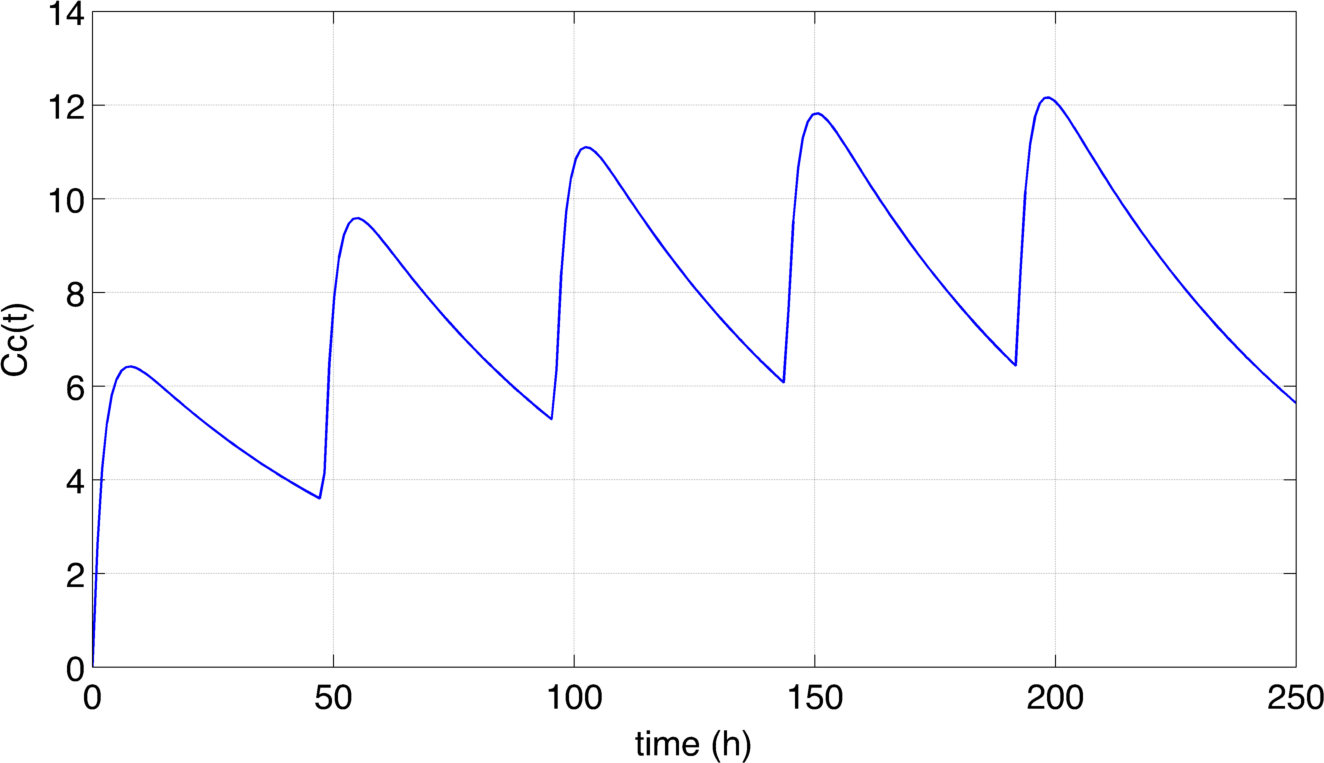
\includegraphics[width=70mm]{pics/example8_singleCc} & 
 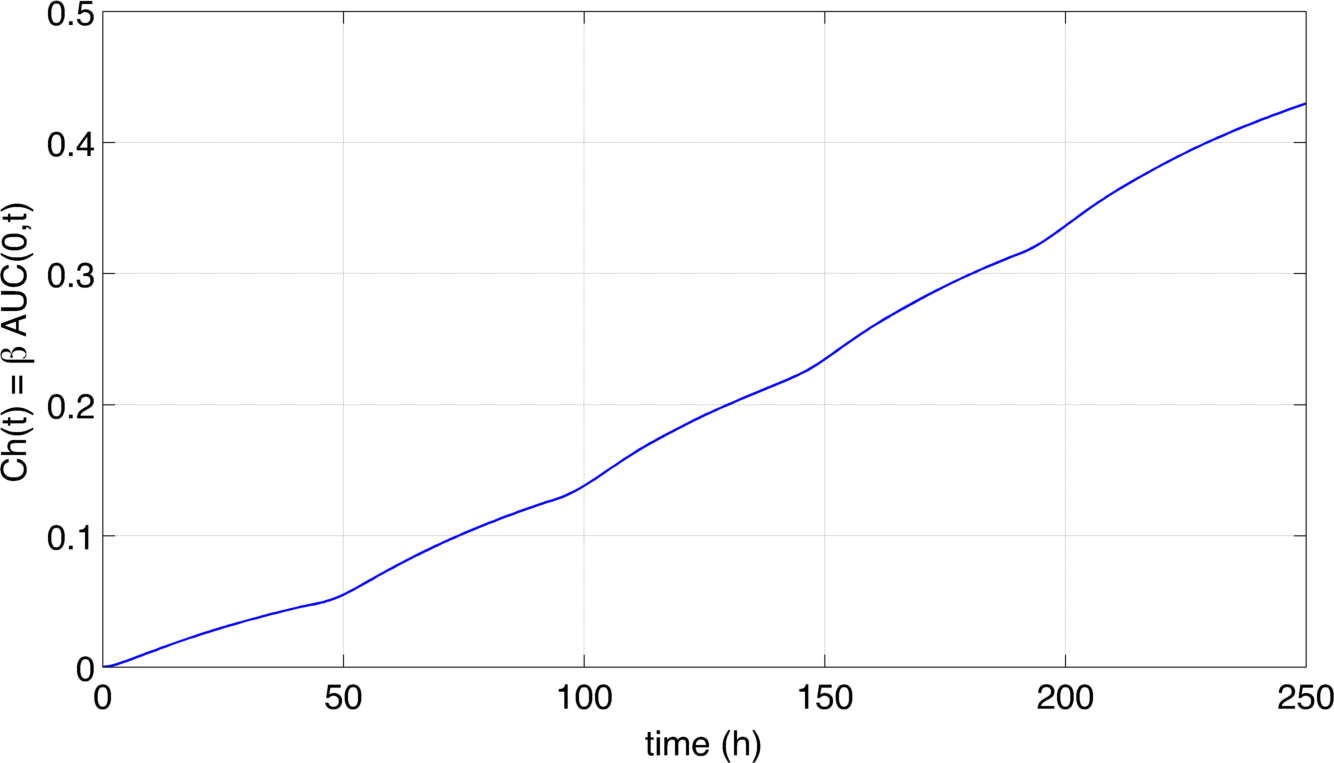
\includegraphics[width=70mm]{pics/example8_singleCh} \\
 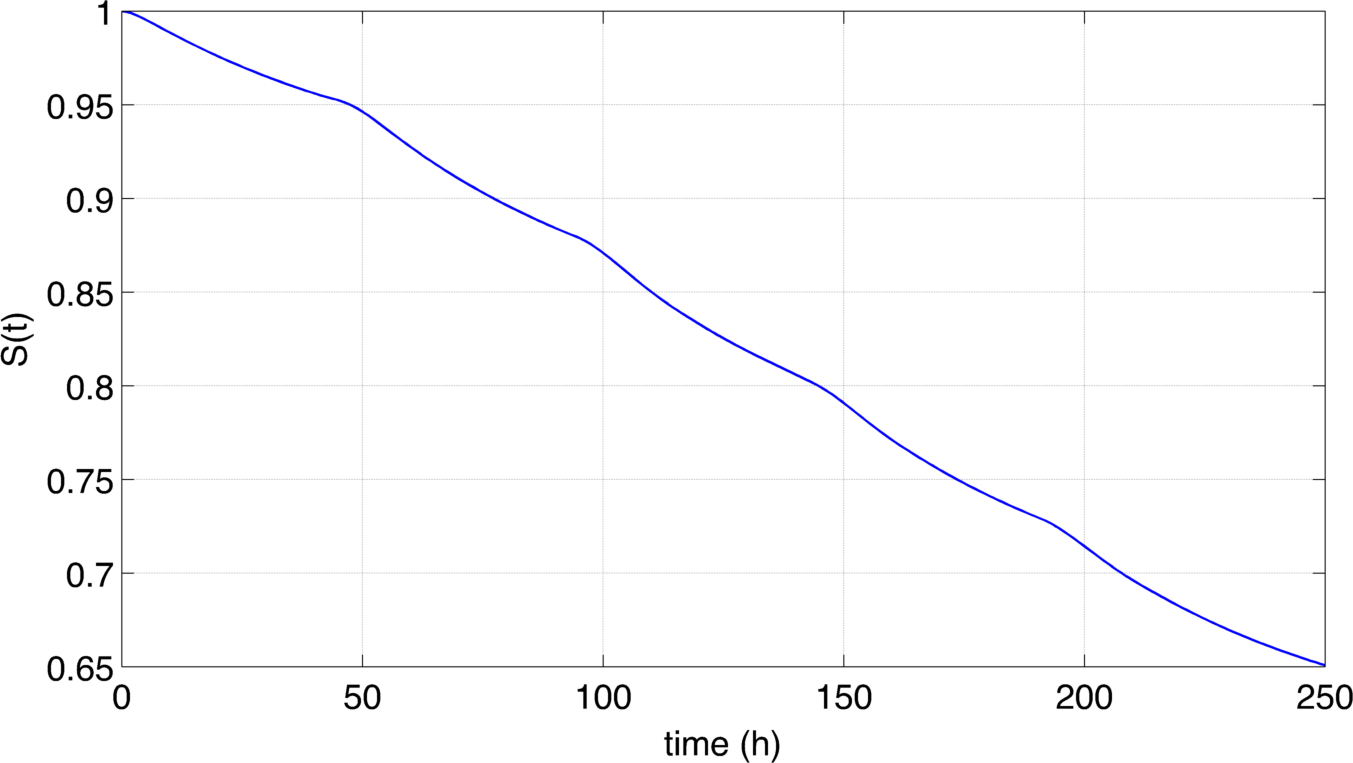
\includegraphics[width=70mm]{pics/example8_singleS} &
\end{tabular}
\caption{Single subject time course for concentration, \emph{Cc}, cumulative hazard, \emph{Ch}, 
and survival function, \emph{S}.}
\end{figure}


\subsubsection{Individual parameters model}
\begin{eqnarray}
beta& \sim&  \mbox{logNormal}(pop_{beta}, \omega_{beta}); \quad \pop_{beta}=0.13,\quad \omega_{beta}=0.2 \nonumber
\end{eqnarray}

\subsubsection{Observation model}
We apply a combined residual error model to the continuous PK output variable 
\var{Cc} and Poisson error distribution for the discrete PD component, defined by \var{Y}, 
as the following table shows 

%\begin{table*}[h!]
\begin{center}
\small
\renewcommand{\arraystretch}{1.1}% 
\begin{tabular*}{0.8\linewidth}{@{\extracolsep{\fill}} >{\bfseries}l l l}\toprule
Output Variable & \textbf{\itshape Cc} &\textbf{\itshape Y}\\\midrule
Observation Name & Concentration & State \\
Units & $\mg/l$ & -- \\
Type & Continuous & Discrete/Categorical \\
Model & Combined & Binomial\\
Parameters 	& $a, b$ 	& $\theta_1$, $\theta_2$\\
%Regressor	& --		& $Cc$ \\
\bottomrule
\end{tabular*}
\end{center}

%%%%%%%%%%%%%%%%%%%%%%%%%%%%%%%%%%%%%%%%%%%%%%%%%%%%%%%%%%%%%%%%
\subsubsection{Modelling Steps}

The PK and PD output variables to be generated by the simulation and
their associated time points are shown below:

\begin{center}
\small
\renewcommand{\arraystretch}{1.1}% 
\begin{tabular*}{0.9\linewidth}{@{\extracolsep{\fill}} >{\bfseries}l c c}\toprule
Output Variable & \textbf{\itshape Cc} &\textbf{\itshape $p1$}\\\midrule
Observation times & [0.5,4 : 4 : 48, 52 : 24 : 192, 192 : 4 : 250] & 0 : 24 : 288\\
\bottomrule
\end{tabular*}
\end{center}


%%%%%%%%%%%%%%%%%%%%%%%%%%%%%%%%%%%%%%%%%%%%%%%%%%%%%%%%%%%%%%%%
\subsection{Observation model}

\lstset{language=XML}
\begin{lstlisting}

\end{lstlisting}

%\begin{figure}
%\centering
%\begin{tabular}{cc}
% 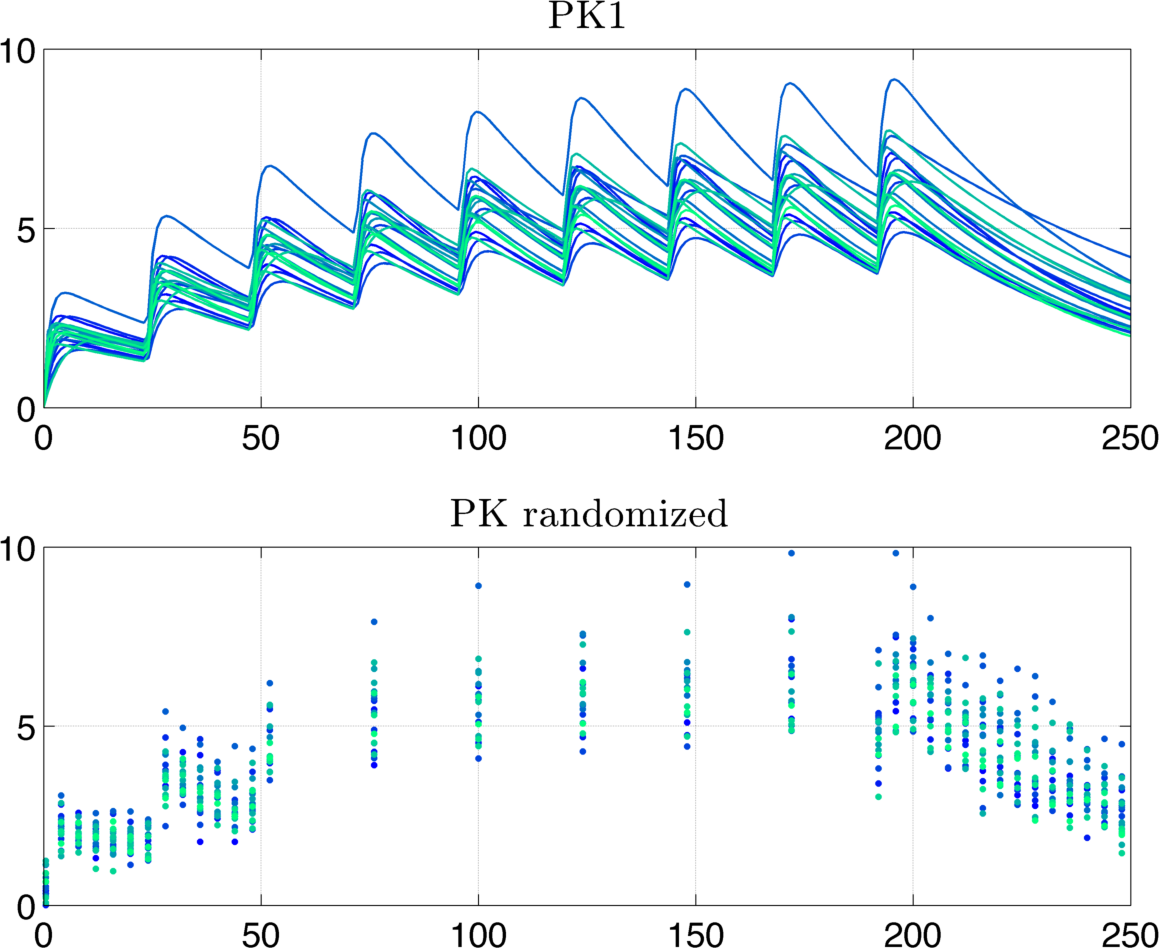
\includegraphics[width=80mm]{pics/example8_PK1_PK2} &
% 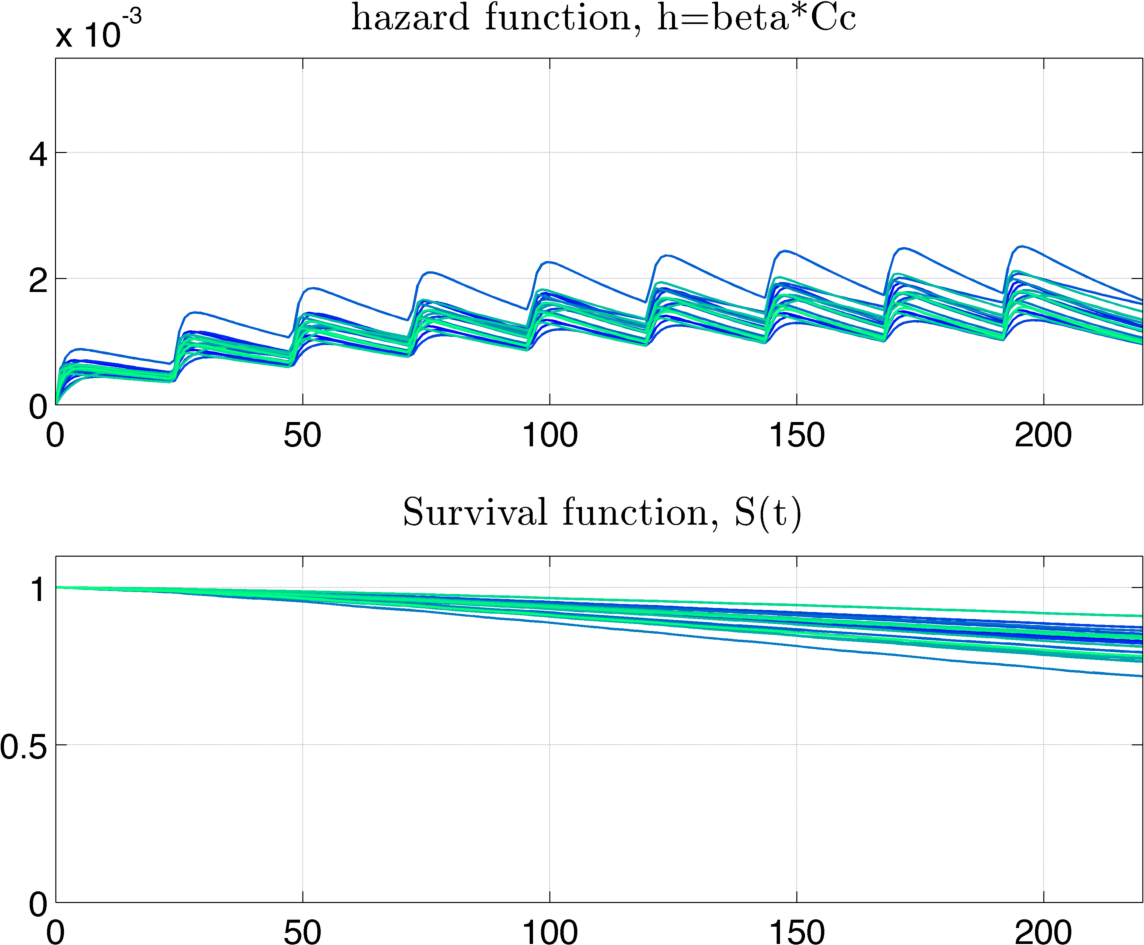
\includegraphics[width=80mm]{pics/example8_hazardPD_S}
%\end{tabular}
%\caption{PK as calculated from the PK model (top left) and with residual error model (bottom left). Hazard and survival function plot, here for arm A (right.)}
%\end{figure}


%%%%%%%%%%%%%%%%%%%%%%%%%%%%%%%%%%%%%%%%%%%%%%%%%%%%%%%%%%%%%%%%
\subsection{NONMEM dataset}
\label{sec:eg8-NONMEMdataset}
The remaining part is the the data and trial design as sourced from the 
NONMEM dataset. Table \ref{tab:example8_dataSet} show a typical dataset required for 
an estimation task.
\begin{table}[htdp]
\begin{center}
\small
\renewcommand{\arraystretch}{1.1}% 
\begin{tabular}{rrrrrrrr}\toprule
ID 	& TIME	& AMT	& Y		& DVID \\ \midrule
1 	& 0 		& 100 	& . 		& . \\ 
1 	& 1 		& . 		& 1	 	& 2 \\ 
1 	& 4 		& . 		& 9.2 	& 1 \\ 
1 	& 8 		& . 		& 0 		& 2 \\ 
1 	& 10		& . 		& 0	 	& 2 \\ 
1 	& 12 	& . 		& 8.5 	& 1 \\ 
1 	& 18 	& . 		& 6.4 	& 1 \\ 
1 	& 24 	& . 		& 1 		& 2 \\ 
2 	& 0 		& 120	&  26 	& . \\ 
2 	& 4 		& . 		& 4.8 	& 1 \\ 
2 	& 8 		& . 		& 0 		& 2 \\ 
2 	& 12 	& . 		& 3.1 	& 1 \\ 
2 	& 18 	& . 		& 2.5 	& 1 \\ 
2 	& 24 	& . 		& 1 		& 2 \\ 
...	& ...		& ...		& ...		& ...	\\ \bottomrule
\end{tabular}
\end{center}
\caption{A dataset used in example for first two subjects.
The additional column DVID is used to specify the type of data. Here, 
DVID =1 is used for a continuous response and DVID =2 for count data.}
\label{tab:example8_dataSet}
\end{table}%







%%% Local Variables:
%%% mode: latex
%%% TeX-master: "../moml-specification"
%%% End:



